\documentclass[11pt,a4paper]{article}
\usepackage[margin=1.25cm, top=1.1cm, bottom=1.3cm]{geometry}
\usepackage[scaled]{helvet}\renewcommand\familydefault{\sfdefault}
\usepackage[T1]{fontenc}
\usepackage{tikz,xcolor,array,tabularx,booktabs,enumitem,multicol,colortbl}
\usetikzlibrary{arrows.meta,shapes.misc}
\pagestyle{empty}
\setlength{\parindent}{0pt}
\definecolor{a34}{HTML}{1F6FB2}
\definecolor{c18}{HTML}{E07B00}
\definecolor{mapbg}{HTML}{F7F5EE}
\definecolor{riverblue}{HTML}{8EC3E6}
\definecolor{tree}{HTML}{9CC48A}
\definecolor{board}{HTML}{1E1E1E}
\definecolor{amber}{HTML}{FFB000}
\tikzset{
  river/.style={riverblue},
  lake/.style={fill=riverblue!70},
  tree/.style={fill=tree},
  busstop/.style={circle, draw=black, fill=white, line width=1pt, inner sep=0pt},
  station/.style={rectangle, draw=black, fill=white, line width=1.2pt, inner sep=0pt},
  inter/.style={circle, draw=black, fill=white, line width=2pt, inner sep=0pt, double=white, double distance=0.6pt},
  badge/.style={rectangle, rounded corners=2pt, fill=#1, text=white, font=\scriptsize\bfseries, inner sep=2pt},
  busA/.style={rectangle, rounded corners=2pt, fill=a34, draw=white, text=white, font=\scriptsize\bfseries, inner sep=1.6pt, line width=0.8pt},
  busC/.style={rectangle, rounded corners=2pt, fill=c18, draw=white, text=white, font=\scriptsize\bfseries, inner sep=1.6pt, line width=0.8pt},
  train/.style={rectangle, rounded corners=3pt, fill=black, draw=white, text=white, font=\scriptsize\bfseries, inner sep=1.6pt, line width=0.8pt},
}
\newcommand{\banner}[2]{\begin{tikzpicture}\node[fill=#1, text=white, font=\large\bfseries, inner xsep=8pt, inner ysep=5pt, minimum width=\linewidth, align=left, text width=\linewidth-16pt] {#2};\end{tikzpicture}}
\newcommand{\ans}[1]{\textcolor{red!75!black}{\bfseries #1}}
\newcommand{\aline}{\rule{2.2cm}{0.4pt}}\newcommand{\sline}{\rule{2.6cm}{0.4pt}}
\renewcommand{\arraystretch}{1.35}
\begin{document}

\begin{center}{\Huge\bfseries Going Places!}\\[2pt]{\large Map of the area \& timetables}\end{center}\vspace{-2pt}
\begin{center}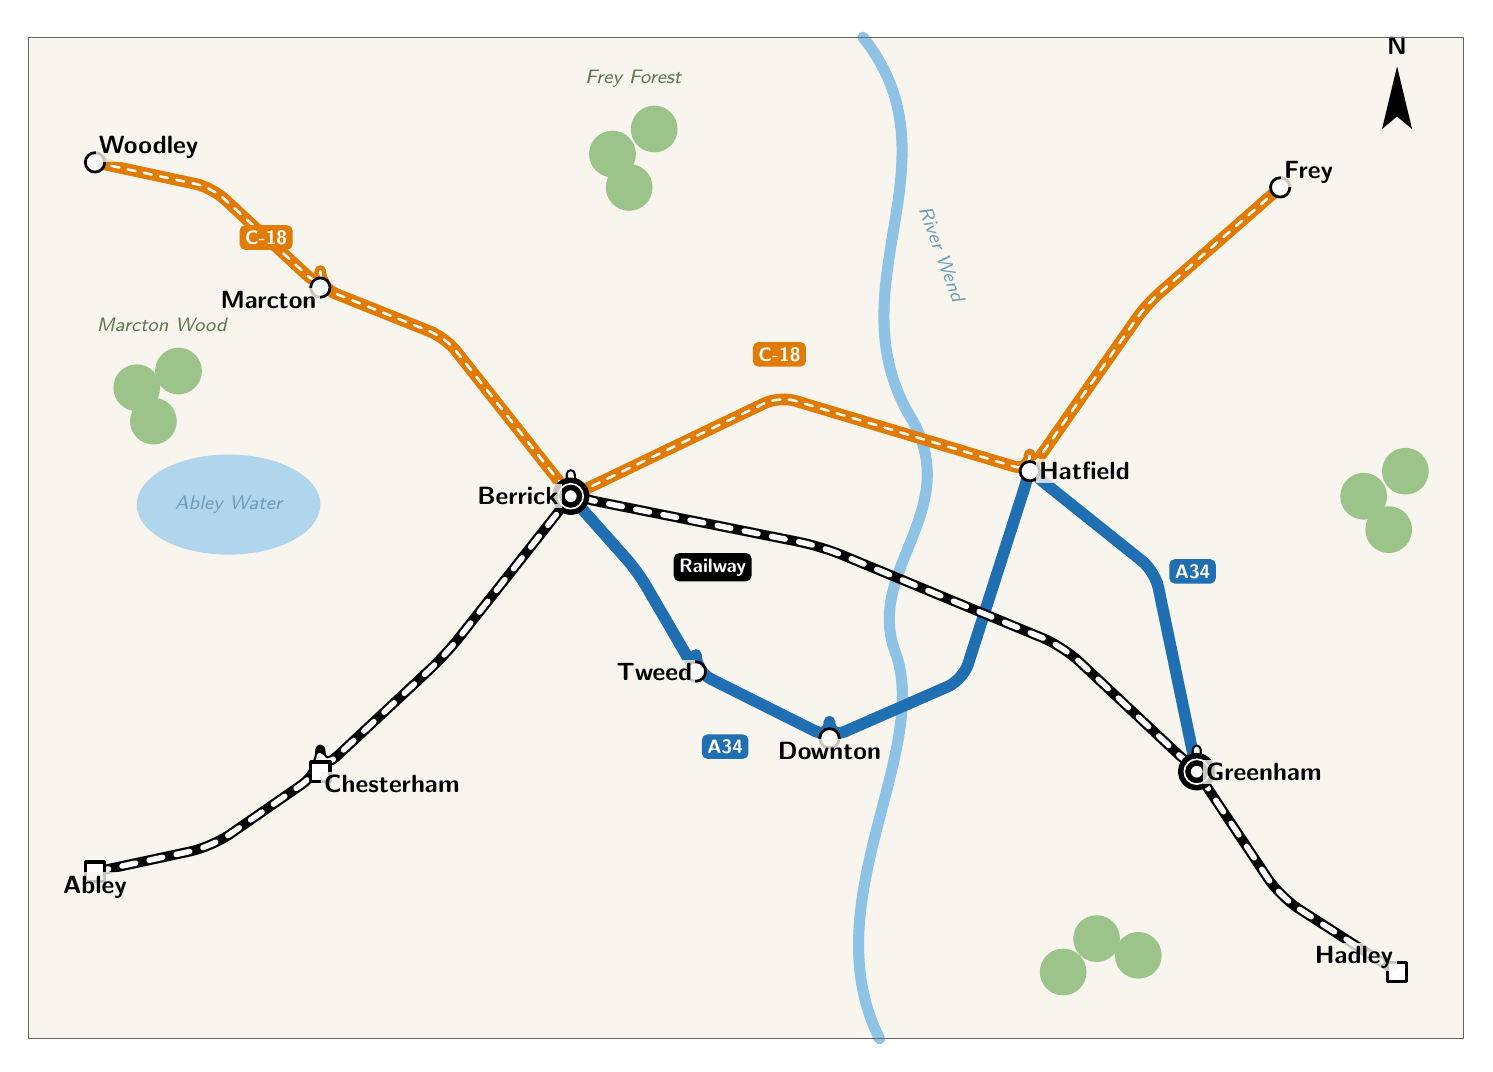
\begin{tikzpicture}[scale=1.06, line cap=round, line join=round]
\fill[mapbg] (0,0) rectangle (17.2,12);
\draw[river, line width=4.0pt] (10.0,12) .. controls (11.2,10.5) and (9.6,9.0) .. (10.6,7.4) .. controls (11.2,6.3) and (10.0,5.6) .. (10.4,4.6) .. controls (10.8,3.4) and (9.4,1.6) .. (10.2,0);
\fill[lake] (2.4,6.4) ellipse (1.1 and 0.6);
\node[font=\scriptsize\itshape, text=riverblue!80!black] at (2.4,6.4) {Abley Water};
\node[font=\scriptsize\itshape, text=riverblue!80!black, rotate=-70] at (10.95,9.4) {River Wend};
\fill[tree] (1.3,7.8) circle (0.28);
\fill[tree] (1.8,8.0) circle (0.28);
\fill[tree] (1.5,7.4) circle (0.28);
\fill[tree] (12.8,1.2) circle (0.28);
\fill[tree] (13.3,1.0) circle (0.28);
\fill[tree] (12.4,0.8) circle (0.28);
\fill[tree] (16.0,6.5) circle (0.28);
\fill[tree] (16.5,6.8) circle (0.28);
\fill[tree] (16.3,6.1) circle (0.28);
\fill[tree] (7.0,10.6) circle (0.28);
\fill[tree] (7.5,10.9) circle (0.28);
\fill[tree] (7.2,10.2) circle (0.28);
\node[font=\scriptsize\itshape, text=tree!60!black] at (1.6,8.55) {Marcton Wood};
\node[font=\scriptsize\itshape, text=tree!60!black] at (7.25,11.5) {Frey Forest};
\draw[a34, line width=4.2pt, rounded corners=6pt] (6.50,6.50) -- (7.30,5.60) -- (8.00,4.40) -- (8.00,4.40) -- (9.60,3.60) -- (9.60,3.60) -- (11.20,4.30) -- (12.00,6.80) -- (12.00,6.80) -- (13.50,5.60) -- (14.00,3.20);
\draw[c18, line width=4.2pt, rounded corners=6pt] (0.80,10.50) -- (2.20,10.20) -- (3.50,9.00) -- (3.50,9.00) -- (5.00,8.40) -- (6.50,6.50) -- (6.50,6.50) -- (9.00,7.70) -- (12.00,6.80) -- (12.00,6.80) -- (13.40,8.80) -- (15.00,10.20);
\draw[white, line width=0.9pt, dash pattern=on 3pt off 3pt, rounded corners=6pt] (0.80,10.50) -- (2.20,10.20) -- (3.50,9.00) -- (3.50,9.00) -- (5.00,8.40) -- (6.50,6.50) -- (6.50,6.50) -- (9.00,7.70) -- (12.00,6.80) -- (12.00,6.80) -- (13.40,8.80) -- (15.00,10.20);
\draw[black, line width=3.6pt, rounded corners=8pt] (0.80,2.00) -- (2.20,2.30) -- (3.50,3.20) -- (3.50,3.20) -- (5.00,4.60) -- (6.50,6.50) -- (6.50,6.50) -- (9.50,5.90) -- (12.40,4.70) -- (14.00,3.20) -- (14.00,3.20) -- (15.00,1.70) -- (16.40,0.80);
\draw[white, line width=2.0pt, dash pattern=on 5pt off 5pt, rounded corners=8pt] (0.80,2.00) -- (2.20,2.30) -- (3.50,3.20) -- (3.50,3.20) -- (5.00,4.60) -- (6.50,6.50) -- (6.50,6.50) -- (9.50,5.90) -- (12.40,4.70) -- (14.00,3.20) -- (14.00,3.20) -- (15.00,1.70) -- (16.40,0.80);
\node[badge=a34] at (8.35,3.5) {A34};
\node[badge=a34] at (13.95,5.6) {A34};
\node[badge=c18] at (9.0,8.2) {C-18};
\node[badge=c18] at (2.85,9.6) {C-18};
\node[badge=black] at (8.2,5.65) {Railway};
\begin{scope}[shift={(16.4,10.9)}]\fill[black] (0,0.75) -- (0.18,0) -- (0,0.15) -- (-0.18,0) -- cycle; \node[font=\bfseries\small] at (0,1.0) {N};\end{scope}
\node[busstop, minimum size=7.0pt] at (0.8,10.5) {};
\node[above right, font=\small\bfseries, fill=mapbg, fill opacity=0.8, text opacity=1, inner sep=1.2pt] at (0.8,10.5) {Woodley};
\node[busstop, minimum size=7.0pt] at (3.5,9.0) {};
\node[below left, font=\small\bfseries, fill=mapbg, fill opacity=0.8, text opacity=1, inner sep=1.2pt] at (3.5,9.0) {Marcton};
\node[inter, minimum size=9.0pt] at (6.5,6.5) {};
\node[left=3pt, font=\small\bfseries, fill=mapbg, fill opacity=0.8, text opacity=1, inner sep=1.2pt] at (6.5,6.5) {Berrick};
\node[busstop, minimum size=7.0pt] at (8.0,4.4) {};
\node[left, font=\small\bfseries, fill=mapbg, fill opacity=0.8, text opacity=1, inner sep=1.2pt] at (8.0,4.4) {Tweed};
\node[busstop, minimum size=7.0pt] at (9.6,3.6) {};
\node[below, font=\small\bfseries, fill=mapbg, fill opacity=0.8, text opacity=1, inner sep=1.2pt] at (9.6,3.6) {Downton};
\node[busstop, minimum size=7.0pt] at (12.0,6.8) {};
\node[right=2pt, font=\small\bfseries, fill=mapbg, fill opacity=0.8, text opacity=1, inner sep=1.2pt] at (12.0,6.8) {Hatfield};
\node[inter, minimum size=9.0pt] at (14.0,3.2) {};
\node[right=2pt, font=\small\bfseries, fill=mapbg, fill opacity=0.8, text opacity=1, inner sep=1.2pt] at (14.0,3.2) {Greenham};
\node[busstop, minimum size=7.0pt] at (15.0,10.2) {};
\node[above right, font=\small\bfseries, fill=mapbg, fill opacity=0.8, text opacity=1, inner sep=1.2pt] at (15.0,10.2) {Frey};
\node[station, minimum size=7.0pt] at (0.8,2.0) {};
\node[below, font=\small\bfseries, fill=mapbg, fill opacity=0.8, text opacity=1, inner sep=1.2pt] at (0.8,2.0) {Abley};
\node[station, minimum size=7.0pt] at (3.5,3.2) {};
\node[below right, font=\small\bfseries, fill=mapbg, fill opacity=0.8, text opacity=1, inner sep=1.2pt] at (3.5,3.2) {Chesterham};
\node[station, minimum size=7.0pt] at (16.4,0.8) {};
\node[above left, font=\small\bfseries, fill=mapbg, fill opacity=0.8, text opacity=1, inner sep=1.2pt] at (16.4,0.8) {Hadley};
\draw[black!60] (0,0) rectangle (17.2,12);
\end{tikzpicture}\\[6pt]{\small 
\begin{tikzpicture}[line cap=round]
\draw[a34, line width=4pt] (0,0) -- (1,0); \node[right] at (1.1,0) {A34 bus};
\draw[c18, line width=4pt] (3.3,0) -- (4.3,0); \draw[white, line width=0.9pt, dash pattern=on 3pt off 3pt] (3.3,0) -- (4.3,0); \node[right] at (4.4,0) {C-18 bus};
\draw[black, line width=3.6pt] (6.7,0) -- (7.7,0); \draw[white, line width=2pt, dash pattern=on 5pt off 5pt] (6.7,0) -- (7.7,0); \node[right] at (7.8,0) {Railway};
\node[busstop, minimum size=7pt] at (10.2,0) {}; \node[right] at (10.35,0) {Bus stop};
\node[station, minimum size=7pt] at (12.4,0) {}; \node[right] at (12.55,0) {Station};
\node[inter, minimum size=9pt] at (14.4,0) {}; \node[right] at (14.6,0) {Change here};
\end{tikzpicture}}\end{center}
\vspace{2pt}\textbf{How it works.} Buses and trains only stop at the places shown in their timetable. If there is a gap in a timetable,
the vehicle \emph{goes straight past} that stop without stopping. (The C-18B uses the same road as the C-18, but does not stop at Berrick or Hatfield.)\par\medskip
{\footnotesize\setlength{\tabcolsep}{4pt}\renewcommand{\arraystretch}{1.1}%
\begin{tabular}[t]{>{\bfseries}l ccc}\multicolumn{4}{l}{\textcolor{a34}{\bfseries A34 bus}}\\\toprule
Berrick & 09:00 & 09:10 & 09:45\\ Tweed & 09:15 & 09:25 & 10:05\\ Downton & 09:21 & 09:31 & 10:15\\ Hatfield & 09:38 & 09:48 & 10:30\\ Greenham & 09:56 & 10:06 & 10:52\\\bottomrule\end{tabular}\hfill
\begin{tabular}[t]{>{\bfseries}l cccc}\multicolumn{5}{l}{\textcolor{c18}{\bfseries C-18 bus}}\\\toprule
 & \bfseries C-18 & \bfseries C-18A & \bfseries C-18B & \bfseries C-18\\\midrule
Woodley & 09:10 & 09:32 & 09:56 & 10:34\\ Marcton & 09:22 & 09:44 & 10:10 & 10:46\\ Berrick & 09:42 & & & 11:09\\ Hatfield & 10:08 & 10:30 & & 11:32\\ Frey & 10:25 & 10:47 & 11:12 & 11:49\\\bottomrule\end{tabular}\hfill
\begin{tabular}[t]{>{\bfseries}l ccccc}\multicolumn{6}{l}{\bfseries Train}\\\toprule
Abley & 08:12 & 08:44 & 08:59 & 09:24 & 09:55\\ Chesterham & 08:24 & 08:56 & & 09:48 & 10:07\\ Berrick & & 09:18 & & 10:01 & 10:29\\ Greenham & 09:32 & & & & 11:10\\ Hadley & 09:58 & 10:30 & 10:19 & & 11:36\\\bottomrule\end{tabular}}
\clearpage

\banner{black!80}{Part A \quad Frozen moments}\par\smallskip
{\small Time has frozen! For each clock, use the timetables to work out where every vehicle is.
\textbf{Draw each vehicle that is on the move on the map} as a small box with its starting time inside (e.g.\ \tikz[baseline=-3pt]\node[busA]{9:00};).
Then fill in the table. If it has not left yet or has finished, write that instead.}\par\medskip

\noindent\begin{minipage}[t]{0.555\linewidth}\vspace{0pt}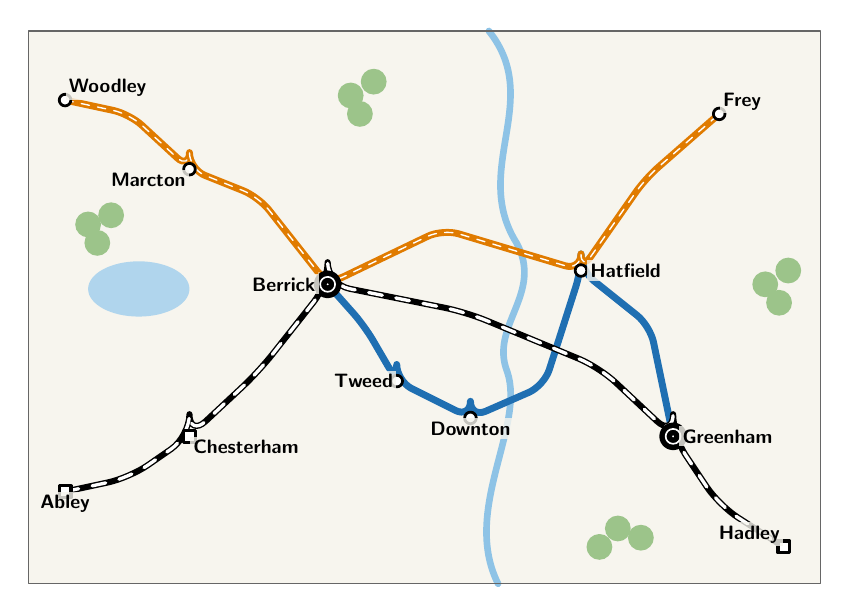
\begin{tikzpicture}[scale=0.585, line cap=round, line join=round]
\fill[mapbg] (0,0) rectangle (17.2,12);
\draw[river, line width=2.4pt] (10.0,12) .. controls (11.2,10.5) and (9.6,9.0) .. (10.6,7.4) .. controls (11.2,6.3) and (10.0,5.6) .. (10.4,4.6) .. controls (10.8,3.4) and (9.4,1.6) .. (10.2,0);
\fill[lake] (2.4,6.4) ellipse (1.1 and 0.6);
\fill[tree] (1.3,7.8) circle (0.28);
\fill[tree] (1.8,8.0) circle (0.28);
\fill[tree] (1.5,7.4) circle (0.28);
\fill[tree] (12.8,1.2) circle (0.28);
\fill[tree] (13.3,1.0) circle (0.28);
\fill[tree] (12.4,0.8) circle (0.28);
\fill[tree] (16.0,6.5) circle (0.28);
\fill[tree] (16.5,6.8) circle (0.28);
\fill[tree] (16.3,6.1) circle (0.28);
\fill[tree] (7.0,10.6) circle (0.28);
\fill[tree] (7.5,10.9) circle (0.28);
\fill[tree] (7.2,10.2) circle (0.28);
\draw[a34, line width=2.5pt, rounded corners=6pt] (6.50,6.50) -- (7.30,5.60) -- (8.00,4.40) -- (8.00,4.40) -- (9.60,3.60) -- (9.60,3.60) -- (11.20,4.30) -- (12.00,6.80) -- (12.00,6.80) -- (13.50,5.60) -- (14.00,3.20);
\draw[c18, line width=2.5pt, rounded corners=6pt] (0.80,10.50) -- (2.20,10.20) -- (3.50,9.00) -- (3.50,9.00) -- (5.00,8.40) -- (6.50,6.50) -- (6.50,6.50) -- (9.00,7.70) -- (12.00,6.80) -- (12.00,6.80) -- (13.40,8.80) -- (15.00,10.20);
\draw[white, line width=0.5pt, dash pattern=on 3pt off 3pt, rounded corners=6pt] (0.80,10.50) -- (2.20,10.20) -- (3.50,9.00) -- (3.50,9.00) -- (5.00,8.40) -- (6.50,6.50) -- (6.50,6.50) -- (9.00,7.70) -- (12.00,6.80) -- (12.00,6.80) -- (13.40,8.80) -- (15.00,10.20);
\draw[black, line width=2.2pt, rounded corners=8pt] (0.80,2.00) -- (2.20,2.30) -- (3.50,3.20) -- (3.50,3.20) -- (5.00,4.60) -- (6.50,6.50) -- (6.50,6.50) -- (9.50,5.90) -- (12.40,4.70) -- (14.00,3.20) -- (14.00,3.20) -- (15.00,1.70) -- (16.40,0.80);
\draw[white, line width=1.2pt, dash pattern=on 5pt off 5pt, rounded corners=8pt] (0.80,2.00) -- (2.20,2.30) -- (3.50,3.20) -- (3.50,3.20) -- (5.00,4.60) -- (6.50,6.50) -- (6.50,6.50) -- (9.50,5.90) -- (12.40,4.70) -- (14.00,3.20) -- (14.00,3.20) -- (15.00,1.70) -- (16.40,0.80);
\node[busstop, minimum size=4.2pt] at (0.8,10.5) {};
\node[above right, font=\scriptsize\bfseries, fill=mapbg, fill opacity=0.8, text opacity=1, inner sep=1.2pt] at (0.8,10.5) {Woodley};
\node[busstop, minimum size=4.2pt] at (3.5,9.0) {};
\node[below left, font=\scriptsize\bfseries, fill=mapbg, fill opacity=0.8, text opacity=1, inner sep=1.2pt] at (3.5,9.0) {Marcton};
\node[inter, minimum size=5.4pt] at (6.5,6.5) {};
\node[left=3pt, font=\scriptsize\bfseries, fill=mapbg, fill opacity=0.8, text opacity=1, inner sep=1.2pt] at (6.5,6.5) {Berrick};
\node[busstop, minimum size=4.2pt] at (8.0,4.4) {};
\node[left, font=\scriptsize\bfseries, fill=mapbg, fill opacity=0.8, text opacity=1, inner sep=1.2pt] at (8.0,4.4) {Tweed};
\node[busstop, minimum size=4.2pt] at (9.6,3.6) {};
\node[below, font=\scriptsize\bfseries, fill=mapbg, fill opacity=0.8, text opacity=1, inner sep=1.2pt] at (9.6,3.6) {Downton};
\node[busstop, minimum size=4.2pt] at (12.0,6.8) {};
\node[right=2pt, font=\scriptsize\bfseries, fill=mapbg, fill opacity=0.8, text opacity=1, inner sep=1.2pt] at (12.0,6.8) {Hatfield};
\node[inter, minimum size=5.4pt] at (14.0,3.2) {};
\node[right=2pt, font=\scriptsize\bfseries, fill=mapbg, fill opacity=0.8, text opacity=1, inner sep=1.2pt] at (14.0,3.2) {Greenham};
\node[busstop, minimum size=4.2pt] at (15.0,10.2) {};
\node[above right, font=\scriptsize\bfseries, fill=mapbg, fill opacity=0.8, text opacity=1, inner sep=1.2pt] at (15.0,10.2) {Frey};
\node[station, minimum size=4.2pt] at (0.8,2.0) {};
\node[below, font=\scriptsize\bfseries, fill=mapbg, fill opacity=0.8, text opacity=1, inner sep=1.2pt] at (0.8,2.0) {Abley};
\node[station, minimum size=4.2pt] at (3.5,3.2) {};
\node[below right, font=\scriptsize\bfseries, fill=mapbg, fill opacity=0.8, text opacity=1, inner sep=1.2pt] at (3.5,3.2) {Chesterham};
\node[station, minimum size=4.2pt] at (16.4,0.8) {};
\node[above left, font=\scriptsize\bfseries, fill=mapbg, fill opacity=0.8, text opacity=1, inner sep=1.2pt] at (16.4,0.8) {Hadley};
\draw[black!60] (0,0) rectangle (17.2,12);
\end{tikzpicture}\end{minipage}\hfill\begin{minipage}[t]{0.425\linewidth}\vspace{0pt}{\large\bfseries 1.}\ \ 
\begin{tikzpicture}[baseline=-3pt]\draw[thick, fill=white] (0,0) circle (0.5);\draw[thick] (0.000,0.360) -- (0.000,0.500);\draw[] (0.215,0.372) -- (0.250,0.433);\draw[] (0.372,0.215) -- (0.433,0.250);\draw[thick] (0.360,0.000) -- (0.500,0.000);\draw[] (0.372,-0.215) -- (0.433,-0.250);\draw[] (0.215,-0.372) -- (0.250,-0.433);\draw[thick] (0.000,-0.360) -- (0.000,-0.500);\draw[] (-0.215,-0.372) -- (-0.250,-0.433);\draw[] (-0.372,-0.215) -- (-0.433,-0.250);\draw[thick] (-0.360,-0.000) -- (-0.500,-0.000);\draw[] (-0.372,0.215) -- (-0.433,0.250);\draw[] (-0.215,0.372) -- (-0.250,0.433);\draw[line width=1.4pt] (0,0) -- (-0.266,0.071);\draw[line width=0.8pt] (0,0) -- (0.000,-0.425);\fill (0,0) circle (1.2pt);\end{tikzpicture}\ \ {\bfseries Frozen at 09:30 --- A34 buses only}\par\smallskip{\small\begin{tabularx}{\linewidth}{>{\raggedright\arraybackslash}p{3.15cm}|X|X}\textbf{Vehicle} & \textbf{Last stop} & \textbf{Next stop}\\ \hline
A34 (09:00 from Berrick) & & \\[6pt] \hline
A34 (09:10 from Berrick) & & \\[6pt] \hline
A34 (09:45 from Berrick) & & \\[6pt] \hline\end{tabularx}}\end{minipage}\par\vspace{9pt}
\noindent\begin{minipage}[t]{0.555\linewidth}\vspace{0pt}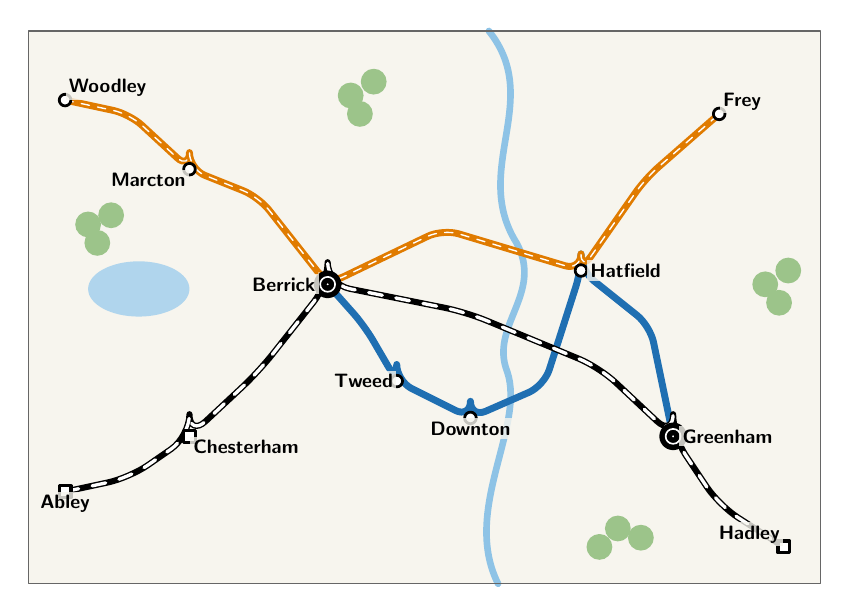
\begin{tikzpicture}[scale=0.585, line cap=round, line join=round]
\fill[mapbg] (0,0) rectangle (17.2,12);
\draw[river, line width=2.4pt] (10.0,12) .. controls (11.2,10.5) and (9.6,9.0) .. (10.6,7.4) .. controls (11.2,6.3) and (10.0,5.6) .. (10.4,4.6) .. controls (10.8,3.4) and (9.4,1.6) .. (10.2,0);
\fill[lake] (2.4,6.4) ellipse (1.1 and 0.6);
\fill[tree] (1.3,7.8) circle (0.28);
\fill[tree] (1.8,8.0) circle (0.28);
\fill[tree] (1.5,7.4) circle (0.28);
\fill[tree] (12.8,1.2) circle (0.28);
\fill[tree] (13.3,1.0) circle (0.28);
\fill[tree] (12.4,0.8) circle (0.28);
\fill[tree] (16.0,6.5) circle (0.28);
\fill[tree] (16.5,6.8) circle (0.28);
\fill[tree] (16.3,6.1) circle (0.28);
\fill[tree] (7.0,10.6) circle (0.28);
\fill[tree] (7.5,10.9) circle (0.28);
\fill[tree] (7.2,10.2) circle (0.28);
\draw[a34, line width=2.5pt, rounded corners=6pt] (6.50,6.50) -- (7.30,5.60) -- (8.00,4.40) -- (8.00,4.40) -- (9.60,3.60) -- (9.60,3.60) -- (11.20,4.30) -- (12.00,6.80) -- (12.00,6.80) -- (13.50,5.60) -- (14.00,3.20);
\draw[c18, line width=2.5pt, rounded corners=6pt] (0.80,10.50) -- (2.20,10.20) -- (3.50,9.00) -- (3.50,9.00) -- (5.00,8.40) -- (6.50,6.50) -- (6.50,6.50) -- (9.00,7.70) -- (12.00,6.80) -- (12.00,6.80) -- (13.40,8.80) -- (15.00,10.20);
\draw[white, line width=0.5pt, dash pattern=on 3pt off 3pt, rounded corners=6pt] (0.80,10.50) -- (2.20,10.20) -- (3.50,9.00) -- (3.50,9.00) -- (5.00,8.40) -- (6.50,6.50) -- (6.50,6.50) -- (9.00,7.70) -- (12.00,6.80) -- (12.00,6.80) -- (13.40,8.80) -- (15.00,10.20);
\draw[black, line width=2.2pt, rounded corners=8pt] (0.80,2.00) -- (2.20,2.30) -- (3.50,3.20) -- (3.50,3.20) -- (5.00,4.60) -- (6.50,6.50) -- (6.50,6.50) -- (9.50,5.90) -- (12.40,4.70) -- (14.00,3.20) -- (14.00,3.20) -- (15.00,1.70) -- (16.40,0.80);
\draw[white, line width=1.2pt, dash pattern=on 5pt off 5pt, rounded corners=8pt] (0.80,2.00) -- (2.20,2.30) -- (3.50,3.20) -- (3.50,3.20) -- (5.00,4.60) -- (6.50,6.50) -- (6.50,6.50) -- (9.50,5.90) -- (12.40,4.70) -- (14.00,3.20) -- (14.00,3.20) -- (15.00,1.70) -- (16.40,0.80);
\node[busstop, minimum size=4.2pt] at (0.8,10.5) {};
\node[above right, font=\scriptsize\bfseries, fill=mapbg, fill opacity=0.8, text opacity=1, inner sep=1.2pt] at (0.8,10.5) {Woodley};
\node[busstop, minimum size=4.2pt] at (3.5,9.0) {};
\node[below left, font=\scriptsize\bfseries, fill=mapbg, fill opacity=0.8, text opacity=1, inner sep=1.2pt] at (3.5,9.0) {Marcton};
\node[inter, minimum size=5.4pt] at (6.5,6.5) {};
\node[left=3pt, font=\scriptsize\bfseries, fill=mapbg, fill opacity=0.8, text opacity=1, inner sep=1.2pt] at (6.5,6.5) {Berrick};
\node[busstop, minimum size=4.2pt] at (8.0,4.4) {};
\node[left, font=\scriptsize\bfseries, fill=mapbg, fill opacity=0.8, text opacity=1, inner sep=1.2pt] at (8.0,4.4) {Tweed};
\node[busstop, minimum size=4.2pt] at (9.6,3.6) {};
\node[below, font=\scriptsize\bfseries, fill=mapbg, fill opacity=0.8, text opacity=1, inner sep=1.2pt] at (9.6,3.6) {Downton};
\node[busstop, minimum size=4.2pt] at (12.0,6.8) {};
\node[right=2pt, font=\scriptsize\bfseries, fill=mapbg, fill opacity=0.8, text opacity=1, inner sep=1.2pt] at (12.0,6.8) {Hatfield};
\node[inter, minimum size=5.4pt] at (14.0,3.2) {};
\node[right=2pt, font=\scriptsize\bfseries, fill=mapbg, fill opacity=0.8, text opacity=1, inner sep=1.2pt] at (14.0,3.2) {Greenham};
\node[busstop, minimum size=4.2pt] at (15.0,10.2) {};
\node[above right, font=\scriptsize\bfseries, fill=mapbg, fill opacity=0.8, text opacity=1, inner sep=1.2pt] at (15.0,10.2) {Frey};
\node[station, minimum size=4.2pt] at (0.8,2.0) {};
\node[below, font=\scriptsize\bfseries, fill=mapbg, fill opacity=0.8, text opacity=1, inner sep=1.2pt] at (0.8,2.0) {Abley};
\node[station, minimum size=4.2pt] at (3.5,3.2) {};
\node[below right, font=\scriptsize\bfseries, fill=mapbg, fill opacity=0.8, text opacity=1, inner sep=1.2pt] at (3.5,3.2) {Chesterham};
\node[station, minimum size=4.2pt] at (16.4,0.8) {};
\node[above left, font=\scriptsize\bfseries, fill=mapbg, fill opacity=0.8, text opacity=1, inner sep=1.2pt] at (16.4,0.8) {Hadley};
\draw[black!60] (0,0) rectangle (17.2,12);
\end{tikzpicture}\end{minipage}\hfill\begin{minipage}[t]{0.425\linewidth}\vspace{0pt}{\large\bfseries 2.}\ \ 
\begin{tikzpicture}[baseline=-3pt]\draw[thick, fill=white] (0,0) circle (0.5);\draw[thick] (0.000,0.360) -- (0.000,0.500);\draw[] (0.215,0.372) -- (0.250,0.433);\draw[] (0.372,0.215) -- (0.433,0.250);\draw[thick] (0.360,0.000) -- (0.500,0.000);\draw[] (0.372,-0.215) -- (0.433,-0.250);\draw[] (0.215,-0.372) -- (0.250,-0.433);\draw[thick] (0.000,-0.360) -- (0.000,-0.500);\draw[] (-0.215,-0.372) -- (-0.250,-0.433);\draw[] (-0.372,-0.215) -- (-0.433,-0.250);\draw[thick] (-0.360,-0.000) -- (-0.500,-0.000);\draw[] (-0.372,0.215) -- (-0.433,0.250);\draw[] (-0.215,0.372) -- (-0.250,0.433);\draw[line width=1.4pt] (0,0) -- (-0.238,0.138);\draw[line width=0.8pt] (0,0) -- (0.000,0.425);\fill (0,0) circle (1.2pt);\end{tikzpicture}\ \ {\bfseries Frozen at 10:00 --- C-18 buses only}\par\smallskip{\small\begin{tabularx}{\linewidth}{>{\raggedright\arraybackslash}p{3.15cm}|X|X}\textbf{Vehicle} & \textbf{Last stop} & \textbf{Next stop}\\ \hline
C-18 (09:10 from Woodley) & & \\[6pt] \hline
C-18A (09:32 from Woodley) & & \\[6pt] \hline
C-18B (09:56 from Woodley) & & \\[6pt] \hline
C-18 (10:34 from Woodley) & & \\[6pt] \hline\end{tabularx}}\end{minipage}\par\vspace{9pt}
\noindent\begin{minipage}[t]{0.555\linewidth}\vspace{0pt}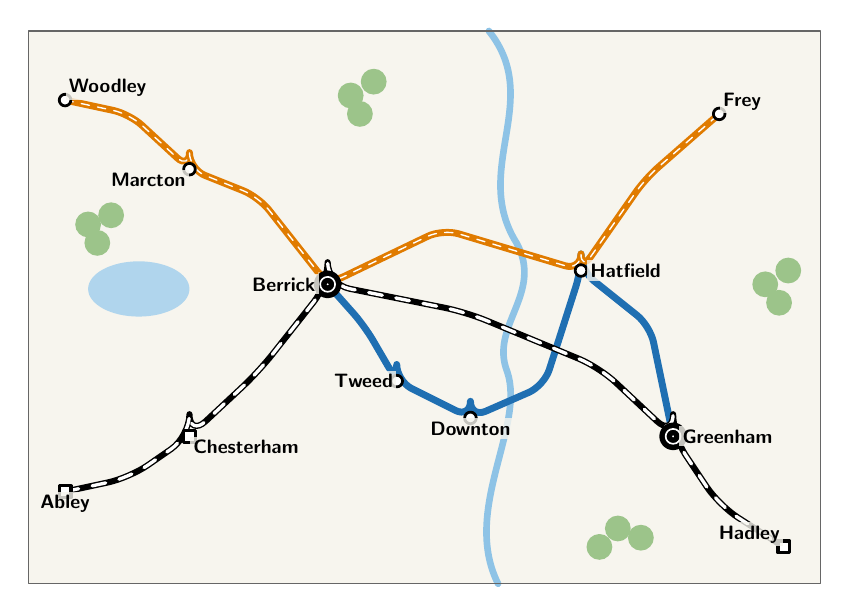
\begin{tikzpicture}[scale=0.585, line cap=round, line join=round]
\fill[mapbg] (0,0) rectangle (17.2,12);
\draw[river, line width=2.4pt] (10.0,12) .. controls (11.2,10.5) and (9.6,9.0) .. (10.6,7.4) .. controls (11.2,6.3) and (10.0,5.6) .. (10.4,4.6) .. controls (10.8,3.4) and (9.4,1.6) .. (10.2,0);
\fill[lake] (2.4,6.4) ellipse (1.1 and 0.6);
\fill[tree] (1.3,7.8) circle (0.28);
\fill[tree] (1.8,8.0) circle (0.28);
\fill[tree] (1.5,7.4) circle (0.28);
\fill[tree] (12.8,1.2) circle (0.28);
\fill[tree] (13.3,1.0) circle (0.28);
\fill[tree] (12.4,0.8) circle (0.28);
\fill[tree] (16.0,6.5) circle (0.28);
\fill[tree] (16.5,6.8) circle (0.28);
\fill[tree] (16.3,6.1) circle (0.28);
\fill[tree] (7.0,10.6) circle (0.28);
\fill[tree] (7.5,10.9) circle (0.28);
\fill[tree] (7.2,10.2) circle (0.28);
\draw[a34, line width=2.5pt, rounded corners=6pt] (6.50,6.50) -- (7.30,5.60) -- (8.00,4.40) -- (8.00,4.40) -- (9.60,3.60) -- (9.60,3.60) -- (11.20,4.30) -- (12.00,6.80) -- (12.00,6.80) -- (13.50,5.60) -- (14.00,3.20);
\draw[c18, line width=2.5pt, rounded corners=6pt] (0.80,10.50) -- (2.20,10.20) -- (3.50,9.00) -- (3.50,9.00) -- (5.00,8.40) -- (6.50,6.50) -- (6.50,6.50) -- (9.00,7.70) -- (12.00,6.80) -- (12.00,6.80) -- (13.40,8.80) -- (15.00,10.20);
\draw[white, line width=0.5pt, dash pattern=on 3pt off 3pt, rounded corners=6pt] (0.80,10.50) -- (2.20,10.20) -- (3.50,9.00) -- (3.50,9.00) -- (5.00,8.40) -- (6.50,6.50) -- (6.50,6.50) -- (9.00,7.70) -- (12.00,6.80) -- (12.00,6.80) -- (13.40,8.80) -- (15.00,10.20);
\draw[black, line width=2.2pt, rounded corners=8pt] (0.80,2.00) -- (2.20,2.30) -- (3.50,3.20) -- (3.50,3.20) -- (5.00,4.60) -- (6.50,6.50) -- (6.50,6.50) -- (9.50,5.90) -- (12.40,4.70) -- (14.00,3.20) -- (14.00,3.20) -- (15.00,1.70) -- (16.40,0.80);
\draw[white, line width=1.2pt, dash pattern=on 5pt off 5pt, rounded corners=8pt] (0.80,2.00) -- (2.20,2.30) -- (3.50,3.20) -- (3.50,3.20) -- (5.00,4.60) -- (6.50,6.50) -- (6.50,6.50) -- (9.50,5.90) -- (12.40,4.70) -- (14.00,3.20) -- (14.00,3.20) -- (15.00,1.70) -- (16.40,0.80);
\node[busstop, minimum size=4.2pt] at (0.8,10.5) {};
\node[above right, font=\scriptsize\bfseries, fill=mapbg, fill opacity=0.8, text opacity=1, inner sep=1.2pt] at (0.8,10.5) {Woodley};
\node[busstop, minimum size=4.2pt] at (3.5,9.0) {};
\node[below left, font=\scriptsize\bfseries, fill=mapbg, fill opacity=0.8, text opacity=1, inner sep=1.2pt] at (3.5,9.0) {Marcton};
\node[inter, minimum size=5.4pt] at (6.5,6.5) {};
\node[left=3pt, font=\scriptsize\bfseries, fill=mapbg, fill opacity=0.8, text opacity=1, inner sep=1.2pt] at (6.5,6.5) {Berrick};
\node[busstop, minimum size=4.2pt] at (8.0,4.4) {};
\node[left, font=\scriptsize\bfseries, fill=mapbg, fill opacity=0.8, text opacity=1, inner sep=1.2pt] at (8.0,4.4) {Tweed};
\node[busstop, minimum size=4.2pt] at (9.6,3.6) {};
\node[below, font=\scriptsize\bfseries, fill=mapbg, fill opacity=0.8, text opacity=1, inner sep=1.2pt] at (9.6,3.6) {Downton};
\node[busstop, minimum size=4.2pt] at (12.0,6.8) {};
\node[right=2pt, font=\scriptsize\bfseries, fill=mapbg, fill opacity=0.8, text opacity=1, inner sep=1.2pt] at (12.0,6.8) {Hatfield};
\node[inter, minimum size=5.4pt] at (14.0,3.2) {};
\node[right=2pt, font=\scriptsize\bfseries, fill=mapbg, fill opacity=0.8, text opacity=1, inner sep=1.2pt] at (14.0,3.2) {Greenham};
\node[busstop, minimum size=4.2pt] at (15.0,10.2) {};
\node[above right, font=\scriptsize\bfseries, fill=mapbg, fill opacity=0.8, text opacity=1, inner sep=1.2pt] at (15.0,10.2) {Frey};
\node[station, minimum size=4.2pt] at (0.8,2.0) {};
\node[below, font=\scriptsize\bfseries, fill=mapbg, fill opacity=0.8, text opacity=1, inner sep=1.2pt] at (0.8,2.0) {Abley};
\node[station, minimum size=4.2pt] at (3.5,3.2) {};
\node[below right, font=\scriptsize\bfseries, fill=mapbg, fill opacity=0.8, text opacity=1, inner sep=1.2pt] at (3.5,3.2) {Chesterham};
\node[station, minimum size=4.2pt] at (16.4,0.8) {};
\node[above left, font=\scriptsize\bfseries, fill=mapbg, fill opacity=0.8, text opacity=1, inner sep=1.2pt] at (16.4,0.8) {Hadley};
\draw[black!60] (0,0) rectangle (17.2,12);
\end{tikzpicture}\end{minipage}\hfill\begin{minipage}[t]{0.425\linewidth}\vspace{0pt}{\large\bfseries 3.}\ \ 
\begin{tikzpicture}[baseline=-3pt]\draw[thick, fill=white] (0,0) circle (0.5);\draw[thick] (0.000,0.360) -- (0.000,0.500);\draw[] (0.215,0.372) -- (0.250,0.433);\draw[] (0.372,0.215) -- (0.433,0.250);\draw[thick] (0.360,0.000) -- (0.500,0.000);\draw[] (0.372,-0.215) -- (0.433,-0.250);\draw[] (0.215,-0.372) -- (0.250,-0.433);\draw[thick] (0.000,-0.360) -- (0.000,-0.500);\draw[] (-0.215,-0.372) -- (-0.250,-0.433);\draw[] (-0.372,-0.215) -- (-0.433,-0.250);\draw[thick] (-0.360,-0.000) -- (-0.500,-0.000);\draw[] (-0.372,0.215) -- (-0.433,0.250);\draw[] (-0.215,0.372) -- (-0.250,0.433);\draw[line width=1.4pt] (0,0) -- (-0.271,0.048);\draw[line width=0.8pt] (0,0) -- (0.368,-0.212);\fill (0,0) circle (1.2pt);\end{tikzpicture}\ \ {\bfseries Frozen at 09:20 --- trains only}\par\smallskip{\small\begin{tabularx}{\linewidth}{>{\raggedright\arraybackslash}p{3.15cm}|X|X}\textbf{Vehicle} & \textbf{Last stop} & \textbf{Next stop}\\ \hline
Train (08:12 from Abley) & & \\[6pt] \hline
Train (08:44 from Abley) & & \\[6pt] \hline
Train (08:59 from Abley) & & \\[6pt] \hline
Train (09:24 from Abley) & & \\[6pt] \hline
Train (09:55 from Abley) & & \\[6pt] \hline\end{tabularx}}\end{minipage}\par\vspace{9pt}
{\small\textbf{Think about it:} At 09:20, the 08:12 train has been travelling for 56 of the 68 minutes from Chesterham to Greenham.
It goes straight through Berrick without stopping. Has it reached Berrick yet? Is it nearer Chesterham or Greenham?}
\clearpage
\banner{black!80}{Part A \quad Frozen moments --- more practice}\par\smallskip
{\small Same again! Draw every vehicle that is on the move, then fill in the table.}\par\medskip

\noindent\begin{minipage}[t]{0.555\linewidth}\vspace{0pt}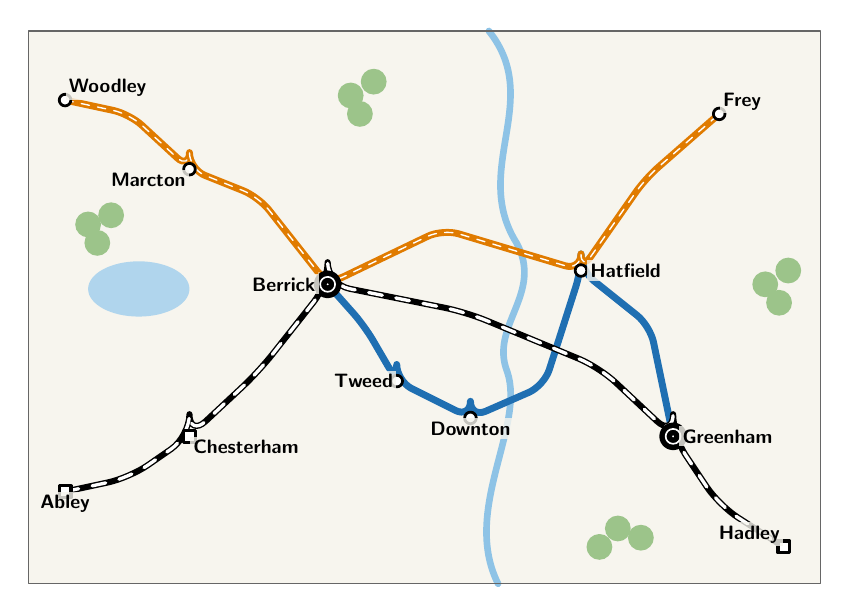
\begin{tikzpicture}[scale=0.585, line cap=round, line join=round]
\fill[mapbg] (0,0) rectangle (17.2,12);
\draw[river, line width=2.4pt] (10.0,12) .. controls (11.2,10.5) and (9.6,9.0) .. (10.6,7.4) .. controls (11.2,6.3) and (10.0,5.6) .. (10.4,4.6) .. controls (10.8,3.4) and (9.4,1.6) .. (10.2,0);
\fill[lake] (2.4,6.4) ellipse (1.1 and 0.6);
\fill[tree] (1.3,7.8) circle (0.28);
\fill[tree] (1.8,8.0) circle (0.28);
\fill[tree] (1.5,7.4) circle (0.28);
\fill[tree] (12.8,1.2) circle (0.28);
\fill[tree] (13.3,1.0) circle (0.28);
\fill[tree] (12.4,0.8) circle (0.28);
\fill[tree] (16.0,6.5) circle (0.28);
\fill[tree] (16.5,6.8) circle (0.28);
\fill[tree] (16.3,6.1) circle (0.28);
\fill[tree] (7.0,10.6) circle (0.28);
\fill[tree] (7.5,10.9) circle (0.28);
\fill[tree] (7.2,10.2) circle (0.28);
\draw[a34, line width=2.5pt, rounded corners=6pt] (6.50,6.50) -- (7.30,5.60) -- (8.00,4.40) -- (8.00,4.40) -- (9.60,3.60) -- (9.60,3.60) -- (11.20,4.30) -- (12.00,6.80) -- (12.00,6.80) -- (13.50,5.60) -- (14.00,3.20);
\draw[c18, line width=2.5pt, rounded corners=6pt] (0.80,10.50) -- (2.20,10.20) -- (3.50,9.00) -- (3.50,9.00) -- (5.00,8.40) -- (6.50,6.50) -- (6.50,6.50) -- (9.00,7.70) -- (12.00,6.80) -- (12.00,6.80) -- (13.40,8.80) -- (15.00,10.20);
\draw[white, line width=0.5pt, dash pattern=on 3pt off 3pt, rounded corners=6pt] (0.80,10.50) -- (2.20,10.20) -- (3.50,9.00) -- (3.50,9.00) -- (5.00,8.40) -- (6.50,6.50) -- (6.50,6.50) -- (9.00,7.70) -- (12.00,6.80) -- (12.00,6.80) -- (13.40,8.80) -- (15.00,10.20);
\draw[black, line width=2.2pt, rounded corners=8pt] (0.80,2.00) -- (2.20,2.30) -- (3.50,3.20) -- (3.50,3.20) -- (5.00,4.60) -- (6.50,6.50) -- (6.50,6.50) -- (9.50,5.90) -- (12.40,4.70) -- (14.00,3.20) -- (14.00,3.20) -- (15.00,1.70) -- (16.40,0.80);
\draw[white, line width=1.2pt, dash pattern=on 5pt off 5pt, rounded corners=8pt] (0.80,2.00) -- (2.20,2.30) -- (3.50,3.20) -- (3.50,3.20) -- (5.00,4.60) -- (6.50,6.50) -- (6.50,6.50) -- (9.50,5.90) -- (12.40,4.70) -- (14.00,3.20) -- (14.00,3.20) -- (15.00,1.70) -- (16.40,0.80);
\node[busstop, minimum size=4.2pt] at (0.8,10.5) {};
\node[above right, font=\scriptsize\bfseries, fill=mapbg, fill opacity=0.8, text opacity=1, inner sep=1.2pt] at (0.8,10.5) {Woodley};
\node[busstop, minimum size=4.2pt] at (3.5,9.0) {};
\node[below left, font=\scriptsize\bfseries, fill=mapbg, fill opacity=0.8, text opacity=1, inner sep=1.2pt] at (3.5,9.0) {Marcton};
\node[inter, minimum size=5.4pt] at (6.5,6.5) {};
\node[left=3pt, font=\scriptsize\bfseries, fill=mapbg, fill opacity=0.8, text opacity=1, inner sep=1.2pt] at (6.5,6.5) {Berrick};
\node[busstop, minimum size=4.2pt] at (8.0,4.4) {};
\node[left, font=\scriptsize\bfseries, fill=mapbg, fill opacity=0.8, text opacity=1, inner sep=1.2pt] at (8.0,4.4) {Tweed};
\node[busstop, minimum size=4.2pt] at (9.6,3.6) {};
\node[below, font=\scriptsize\bfseries, fill=mapbg, fill opacity=0.8, text opacity=1, inner sep=1.2pt] at (9.6,3.6) {Downton};
\node[busstop, minimum size=4.2pt] at (12.0,6.8) {};
\node[right=2pt, font=\scriptsize\bfseries, fill=mapbg, fill opacity=0.8, text opacity=1, inner sep=1.2pt] at (12.0,6.8) {Hatfield};
\node[inter, minimum size=5.4pt] at (14.0,3.2) {};
\node[right=2pt, font=\scriptsize\bfseries, fill=mapbg, fill opacity=0.8, text opacity=1, inner sep=1.2pt] at (14.0,3.2) {Greenham};
\node[busstop, minimum size=4.2pt] at (15.0,10.2) {};
\node[above right, font=\scriptsize\bfseries, fill=mapbg, fill opacity=0.8, text opacity=1, inner sep=1.2pt] at (15.0,10.2) {Frey};
\node[station, minimum size=4.2pt] at (0.8,2.0) {};
\node[below, font=\scriptsize\bfseries, fill=mapbg, fill opacity=0.8, text opacity=1, inner sep=1.2pt] at (0.8,2.0) {Abley};
\node[station, minimum size=4.2pt] at (3.5,3.2) {};
\node[below right, font=\scriptsize\bfseries, fill=mapbg, fill opacity=0.8, text opacity=1, inner sep=1.2pt] at (3.5,3.2) {Chesterham};
\node[station, minimum size=4.2pt] at (16.4,0.8) {};
\node[above left, font=\scriptsize\bfseries, fill=mapbg, fill opacity=0.8, text opacity=1, inner sep=1.2pt] at (16.4,0.8) {Hadley};
\draw[black!60] (0,0) rectangle (17.2,12);
\end{tikzpicture}\end{minipage}\hfill\begin{minipage}[t]{0.425\linewidth}\vspace{0pt}{\large\bfseries 4.}\ \ 
\begin{tikzpicture}[baseline=-3pt]\draw[thick, fill=white] (0,0) circle (0.5);\draw[thick] (0.000,0.360) -- (0.000,0.500);\draw[] (0.215,0.372) -- (0.250,0.433);\draw[] (0.372,0.215) -- (0.433,0.250);\draw[thick] (0.360,0.000) -- (0.500,0.000);\draw[] (0.372,-0.215) -- (0.433,-0.250);\draw[] (0.215,-0.372) -- (0.250,-0.433);\draw[thick] (0.000,-0.360) -- (0.000,-0.500);\draw[] (-0.215,-0.372) -- (-0.250,-0.433);\draw[] (-0.372,-0.215) -- (-0.433,-0.250);\draw[thick] (-0.360,-0.000) -- (-0.500,-0.000);\draw[] (-0.372,0.215) -- (-0.433,0.250);\draw[] (-0.215,0.372) -- (-0.250,0.433);\draw[line width=1.4pt] (0,0) -- (-0.249,0.116);\draw[line width=0.8pt] (0,0) -- (-0.368,0.213);\fill (0,0) circle (1.2pt);\end{tikzpicture}\ \ {\bfseries Frozen at 09:50 --- A34 buses only}\par\smallskip{\small\begin{tabularx}{\linewidth}{>{\raggedright\arraybackslash}p{3.15cm}|X|X}\textbf{Vehicle} & \textbf{Last stop} & \textbf{Next stop}\\ \hline
A34 (09:00 from Berrick) & & \\[6pt] \hline
A34 (09:10 from Berrick) & & \\[6pt] \hline
A34 (09:45 from Berrick) & & \\[6pt] \hline\end{tabularx}}\end{minipage}\par\vspace{9pt}
\noindent\begin{minipage}[t]{0.555\linewidth}\vspace{0pt}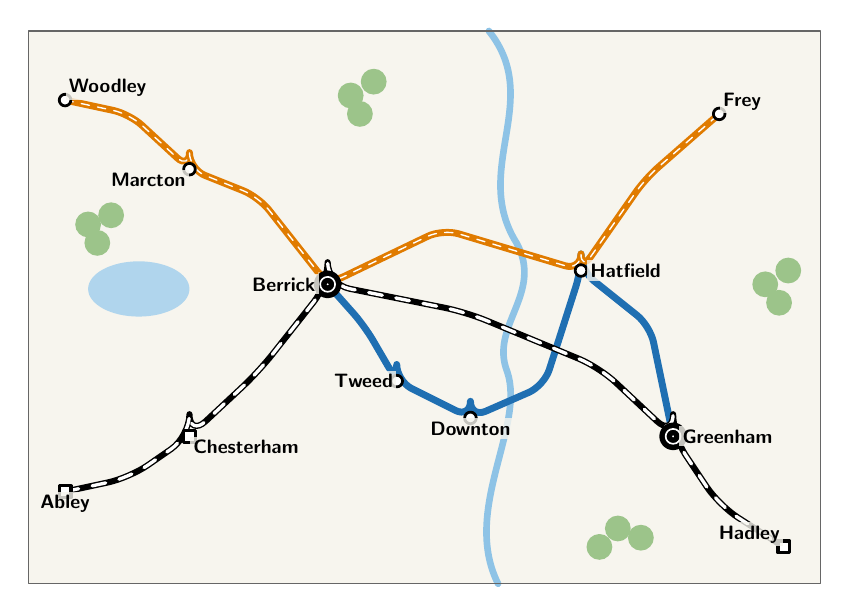
\begin{tikzpicture}[scale=0.585, line cap=round, line join=round]
\fill[mapbg] (0,0) rectangle (17.2,12);
\draw[river, line width=2.4pt] (10.0,12) .. controls (11.2,10.5) and (9.6,9.0) .. (10.6,7.4) .. controls (11.2,6.3) and (10.0,5.6) .. (10.4,4.6) .. controls (10.8,3.4) and (9.4,1.6) .. (10.2,0);
\fill[lake] (2.4,6.4) ellipse (1.1 and 0.6);
\fill[tree] (1.3,7.8) circle (0.28);
\fill[tree] (1.8,8.0) circle (0.28);
\fill[tree] (1.5,7.4) circle (0.28);
\fill[tree] (12.8,1.2) circle (0.28);
\fill[tree] (13.3,1.0) circle (0.28);
\fill[tree] (12.4,0.8) circle (0.28);
\fill[tree] (16.0,6.5) circle (0.28);
\fill[tree] (16.5,6.8) circle (0.28);
\fill[tree] (16.3,6.1) circle (0.28);
\fill[tree] (7.0,10.6) circle (0.28);
\fill[tree] (7.5,10.9) circle (0.28);
\fill[tree] (7.2,10.2) circle (0.28);
\draw[a34, line width=2.5pt, rounded corners=6pt] (6.50,6.50) -- (7.30,5.60) -- (8.00,4.40) -- (8.00,4.40) -- (9.60,3.60) -- (9.60,3.60) -- (11.20,4.30) -- (12.00,6.80) -- (12.00,6.80) -- (13.50,5.60) -- (14.00,3.20);
\draw[c18, line width=2.5pt, rounded corners=6pt] (0.80,10.50) -- (2.20,10.20) -- (3.50,9.00) -- (3.50,9.00) -- (5.00,8.40) -- (6.50,6.50) -- (6.50,6.50) -- (9.00,7.70) -- (12.00,6.80) -- (12.00,6.80) -- (13.40,8.80) -- (15.00,10.20);
\draw[white, line width=0.5pt, dash pattern=on 3pt off 3pt, rounded corners=6pt] (0.80,10.50) -- (2.20,10.20) -- (3.50,9.00) -- (3.50,9.00) -- (5.00,8.40) -- (6.50,6.50) -- (6.50,6.50) -- (9.00,7.70) -- (12.00,6.80) -- (12.00,6.80) -- (13.40,8.80) -- (15.00,10.20);
\draw[black, line width=2.2pt, rounded corners=8pt] (0.80,2.00) -- (2.20,2.30) -- (3.50,3.20) -- (3.50,3.20) -- (5.00,4.60) -- (6.50,6.50) -- (6.50,6.50) -- (9.50,5.90) -- (12.40,4.70) -- (14.00,3.20) -- (14.00,3.20) -- (15.00,1.70) -- (16.40,0.80);
\draw[white, line width=1.2pt, dash pattern=on 5pt off 5pt, rounded corners=8pt] (0.80,2.00) -- (2.20,2.30) -- (3.50,3.20) -- (3.50,3.20) -- (5.00,4.60) -- (6.50,6.50) -- (6.50,6.50) -- (9.50,5.90) -- (12.40,4.70) -- (14.00,3.20) -- (14.00,3.20) -- (15.00,1.70) -- (16.40,0.80);
\node[busstop, minimum size=4.2pt] at (0.8,10.5) {};
\node[above right, font=\scriptsize\bfseries, fill=mapbg, fill opacity=0.8, text opacity=1, inner sep=1.2pt] at (0.8,10.5) {Woodley};
\node[busstop, minimum size=4.2pt] at (3.5,9.0) {};
\node[below left, font=\scriptsize\bfseries, fill=mapbg, fill opacity=0.8, text opacity=1, inner sep=1.2pt] at (3.5,9.0) {Marcton};
\node[inter, minimum size=5.4pt] at (6.5,6.5) {};
\node[left=3pt, font=\scriptsize\bfseries, fill=mapbg, fill opacity=0.8, text opacity=1, inner sep=1.2pt] at (6.5,6.5) {Berrick};
\node[busstop, minimum size=4.2pt] at (8.0,4.4) {};
\node[left, font=\scriptsize\bfseries, fill=mapbg, fill opacity=0.8, text opacity=1, inner sep=1.2pt] at (8.0,4.4) {Tweed};
\node[busstop, minimum size=4.2pt] at (9.6,3.6) {};
\node[below, font=\scriptsize\bfseries, fill=mapbg, fill opacity=0.8, text opacity=1, inner sep=1.2pt] at (9.6,3.6) {Downton};
\node[busstop, minimum size=4.2pt] at (12.0,6.8) {};
\node[right=2pt, font=\scriptsize\bfseries, fill=mapbg, fill opacity=0.8, text opacity=1, inner sep=1.2pt] at (12.0,6.8) {Hatfield};
\node[inter, minimum size=5.4pt] at (14.0,3.2) {};
\node[right=2pt, font=\scriptsize\bfseries, fill=mapbg, fill opacity=0.8, text opacity=1, inner sep=1.2pt] at (14.0,3.2) {Greenham};
\node[busstop, minimum size=4.2pt] at (15.0,10.2) {};
\node[above right, font=\scriptsize\bfseries, fill=mapbg, fill opacity=0.8, text opacity=1, inner sep=1.2pt] at (15.0,10.2) {Frey};
\node[station, minimum size=4.2pt] at (0.8,2.0) {};
\node[below, font=\scriptsize\bfseries, fill=mapbg, fill opacity=0.8, text opacity=1, inner sep=1.2pt] at (0.8,2.0) {Abley};
\node[station, minimum size=4.2pt] at (3.5,3.2) {};
\node[below right, font=\scriptsize\bfseries, fill=mapbg, fill opacity=0.8, text opacity=1, inner sep=1.2pt] at (3.5,3.2) {Chesterham};
\node[station, minimum size=4.2pt] at (16.4,0.8) {};
\node[above left, font=\scriptsize\bfseries, fill=mapbg, fill opacity=0.8, text opacity=1, inner sep=1.2pt] at (16.4,0.8) {Hadley};
\draw[black!60] (0,0) rectangle (17.2,12);
\end{tikzpicture}\end{minipage}\hfill\begin{minipage}[t]{0.425\linewidth}\vspace{0pt}{\large\bfseries 5.}\ \ 
\begin{tikzpicture}[baseline=-3pt]\draw[thick, fill=white] (0,0) circle (0.5);\draw[thick] (0.000,0.360) -- (0.000,0.500);\draw[] (0.215,0.372) -- (0.250,0.433);\draw[] (0.372,0.215) -- (0.433,0.250);\draw[thick] (0.360,0.000) -- (0.500,0.000);\draw[] (0.372,-0.215) -- (0.433,-0.250);\draw[] (0.215,-0.372) -- (0.250,-0.433);\draw[thick] (0.000,-0.360) -- (0.000,-0.500);\draw[] (-0.215,-0.372) -- (-0.250,-0.433);\draw[] (-0.372,-0.215) -- (-0.433,-0.250);\draw[thick] (-0.360,-0.000) -- (-0.500,-0.000);\draw[] (-0.372,0.215) -- (-0.433,0.250);\draw[] (-0.215,0.372) -- (-0.250,0.433);\draw[line width=1.4pt] (0,0) -- (-0.177,0.211);\draw[line width=0.8pt] (0,0) -- (-0.368,-0.212);\fill (0,0) circle (1.2pt);\end{tikzpicture}\ \ {\bfseries Frozen at 10:40 --- C-18 buses only}\par\smallskip{\small\begin{tabularx}{\linewidth}{>{\raggedright\arraybackslash}p{3.15cm}|X|X}\textbf{Vehicle} & \textbf{Last stop} & \textbf{Next stop}\\ \hline
C-18 (09:10 from Woodley) & & \\[6pt] \hline
C-18A (09:32 from Woodley) & & \\[6pt] \hline
C-18B (09:56 from Woodley) & & \\[6pt] \hline
C-18 (10:34 from Woodley) & & \\[6pt] \hline\end{tabularx}}\end{minipage}\par\vspace{9pt}
\noindent\begin{minipage}[t]{0.555\linewidth}\vspace{0pt}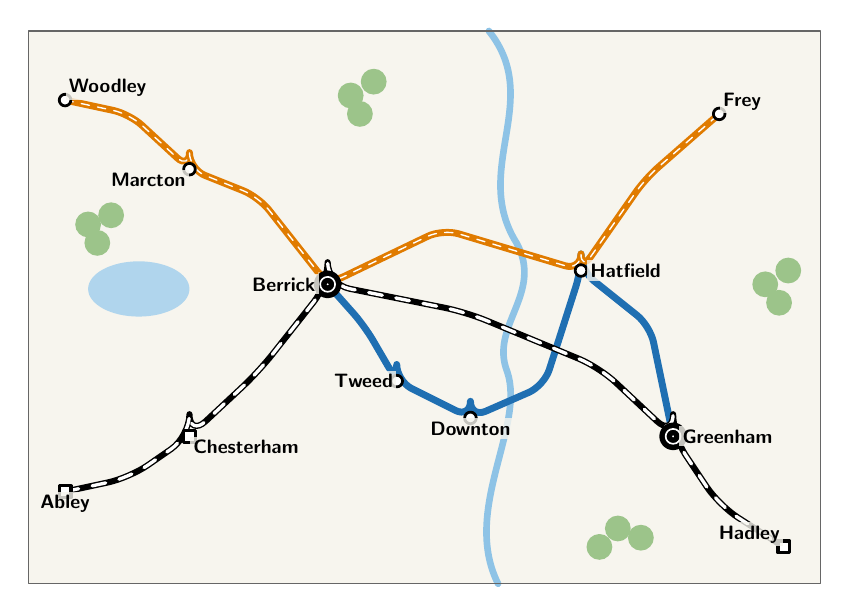
\begin{tikzpicture}[scale=0.585, line cap=round, line join=round]
\fill[mapbg] (0,0) rectangle (17.2,12);
\draw[river, line width=2.4pt] (10.0,12) .. controls (11.2,10.5) and (9.6,9.0) .. (10.6,7.4) .. controls (11.2,6.3) and (10.0,5.6) .. (10.4,4.6) .. controls (10.8,3.4) and (9.4,1.6) .. (10.2,0);
\fill[lake] (2.4,6.4) ellipse (1.1 and 0.6);
\fill[tree] (1.3,7.8) circle (0.28);
\fill[tree] (1.8,8.0) circle (0.28);
\fill[tree] (1.5,7.4) circle (0.28);
\fill[tree] (12.8,1.2) circle (0.28);
\fill[tree] (13.3,1.0) circle (0.28);
\fill[tree] (12.4,0.8) circle (0.28);
\fill[tree] (16.0,6.5) circle (0.28);
\fill[tree] (16.5,6.8) circle (0.28);
\fill[tree] (16.3,6.1) circle (0.28);
\fill[tree] (7.0,10.6) circle (0.28);
\fill[tree] (7.5,10.9) circle (0.28);
\fill[tree] (7.2,10.2) circle (0.28);
\draw[a34, line width=2.5pt, rounded corners=6pt] (6.50,6.50) -- (7.30,5.60) -- (8.00,4.40) -- (8.00,4.40) -- (9.60,3.60) -- (9.60,3.60) -- (11.20,4.30) -- (12.00,6.80) -- (12.00,6.80) -- (13.50,5.60) -- (14.00,3.20);
\draw[c18, line width=2.5pt, rounded corners=6pt] (0.80,10.50) -- (2.20,10.20) -- (3.50,9.00) -- (3.50,9.00) -- (5.00,8.40) -- (6.50,6.50) -- (6.50,6.50) -- (9.00,7.70) -- (12.00,6.80) -- (12.00,6.80) -- (13.40,8.80) -- (15.00,10.20);
\draw[white, line width=0.5pt, dash pattern=on 3pt off 3pt, rounded corners=6pt] (0.80,10.50) -- (2.20,10.20) -- (3.50,9.00) -- (3.50,9.00) -- (5.00,8.40) -- (6.50,6.50) -- (6.50,6.50) -- (9.00,7.70) -- (12.00,6.80) -- (12.00,6.80) -- (13.40,8.80) -- (15.00,10.20);
\draw[black, line width=2.2pt, rounded corners=8pt] (0.80,2.00) -- (2.20,2.30) -- (3.50,3.20) -- (3.50,3.20) -- (5.00,4.60) -- (6.50,6.50) -- (6.50,6.50) -- (9.50,5.90) -- (12.40,4.70) -- (14.00,3.20) -- (14.00,3.20) -- (15.00,1.70) -- (16.40,0.80);
\draw[white, line width=1.2pt, dash pattern=on 5pt off 5pt, rounded corners=8pt] (0.80,2.00) -- (2.20,2.30) -- (3.50,3.20) -- (3.50,3.20) -- (5.00,4.60) -- (6.50,6.50) -- (6.50,6.50) -- (9.50,5.90) -- (12.40,4.70) -- (14.00,3.20) -- (14.00,3.20) -- (15.00,1.70) -- (16.40,0.80);
\node[busstop, minimum size=4.2pt] at (0.8,10.5) {};
\node[above right, font=\scriptsize\bfseries, fill=mapbg, fill opacity=0.8, text opacity=1, inner sep=1.2pt] at (0.8,10.5) {Woodley};
\node[busstop, minimum size=4.2pt] at (3.5,9.0) {};
\node[below left, font=\scriptsize\bfseries, fill=mapbg, fill opacity=0.8, text opacity=1, inner sep=1.2pt] at (3.5,9.0) {Marcton};
\node[inter, minimum size=5.4pt] at (6.5,6.5) {};
\node[left=3pt, font=\scriptsize\bfseries, fill=mapbg, fill opacity=0.8, text opacity=1, inner sep=1.2pt] at (6.5,6.5) {Berrick};
\node[busstop, minimum size=4.2pt] at (8.0,4.4) {};
\node[left, font=\scriptsize\bfseries, fill=mapbg, fill opacity=0.8, text opacity=1, inner sep=1.2pt] at (8.0,4.4) {Tweed};
\node[busstop, minimum size=4.2pt] at (9.6,3.6) {};
\node[below, font=\scriptsize\bfseries, fill=mapbg, fill opacity=0.8, text opacity=1, inner sep=1.2pt] at (9.6,3.6) {Downton};
\node[busstop, minimum size=4.2pt] at (12.0,6.8) {};
\node[right=2pt, font=\scriptsize\bfseries, fill=mapbg, fill opacity=0.8, text opacity=1, inner sep=1.2pt] at (12.0,6.8) {Hatfield};
\node[inter, minimum size=5.4pt] at (14.0,3.2) {};
\node[right=2pt, font=\scriptsize\bfseries, fill=mapbg, fill opacity=0.8, text opacity=1, inner sep=1.2pt] at (14.0,3.2) {Greenham};
\node[busstop, minimum size=4.2pt] at (15.0,10.2) {};
\node[above right, font=\scriptsize\bfseries, fill=mapbg, fill opacity=0.8, text opacity=1, inner sep=1.2pt] at (15.0,10.2) {Frey};
\node[station, minimum size=4.2pt] at (0.8,2.0) {};
\node[below, font=\scriptsize\bfseries, fill=mapbg, fill opacity=0.8, text opacity=1, inner sep=1.2pt] at (0.8,2.0) {Abley};
\node[station, minimum size=4.2pt] at (3.5,3.2) {};
\node[below right, font=\scriptsize\bfseries, fill=mapbg, fill opacity=0.8, text opacity=1, inner sep=1.2pt] at (3.5,3.2) {Chesterham};
\node[station, minimum size=4.2pt] at (16.4,0.8) {};
\node[above left, font=\scriptsize\bfseries, fill=mapbg, fill opacity=0.8, text opacity=1, inner sep=1.2pt] at (16.4,0.8) {Hadley};
\draw[black!60] (0,0) rectangle (17.2,12);
\end{tikzpicture}\end{minipage}\hfill\begin{minipage}[t]{0.425\linewidth}\vspace{0pt}{\large\bfseries 6.}\ \ 
\begin{tikzpicture}[baseline=-3pt]\draw[thick, fill=white] (0,0) circle (0.5);\draw[thick] (0.000,0.360) -- (0.000,0.500);\draw[] (0.215,0.372) -- (0.250,0.433);\draw[] (0.372,0.215) -- (0.433,0.250);\draw[thick] (0.360,0.000) -- (0.500,0.000);\draw[] (0.372,-0.215) -- (0.433,-0.250);\draw[] (0.215,-0.372) -- (0.250,-0.433);\draw[thick] (0.000,-0.360) -- (0.000,-0.500);\draw[] (-0.215,-0.372) -- (-0.250,-0.433);\draw[] (-0.372,-0.215) -- (-0.433,-0.250);\draw[thick] (-0.360,-0.000) -- (-0.500,-0.000);\draw[] (-0.372,0.215) -- (-0.433,0.250);\draw[] (-0.215,0.372) -- (-0.250,0.433);\draw[line width=1.4pt] (0,0) -- (-0.238,0.138);\draw[line width=0.8pt] (0,0) -- (0.000,0.425);\fill (0,0) circle (1.2pt);\end{tikzpicture}\ \ {\bfseries Frozen at 10:00 --- trains only}\par\smallskip{\small\begin{tabularx}{\linewidth}{>{\raggedright\arraybackslash}p{3.15cm}|X|X}\textbf{Vehicle} & \textbf{Last stop} & \textbf{Next stop}\\ \hline
Train (08:12 from Abley) & & \\[6pt] \hline
Train (08:44 from Abley) & & \\[6pt] \hline
Train (08:59 from Abley) & & \\[6pt] \hline
Train (09:24 from Abley) & & \\[6pt] \hline
Train (09:55 from Abley) & & \\[6pt] \hline\end{tabularx}}\end{minipage}\par\vspace{9pt}
{\small\textbf{Think about it:} At 09:50, two A34 buses are on the same stretch of road. Which one is in front?
How many minutes behind is the other one? Will it ever catch up?}
\clearpage
\banner{black!80}{Part A \quad Frozen moments --- Challenge: everything at once}\par\medskip
\noindent\begin{minipage}[c]{0.2\linewidth}\centering 
\begin{tikzpicture}[baseline=-3pt]\draw[thick, fill=white] (0,0) circle (0.85);\draw[thick] (0.000,0.710) -- (0.000,0.850);\draw[] (0.390,0.675) -- (0.425,0.736);\draw[] (0.675,0.390) -- (0.736,0.425);\draw[thick] (0.710,0.000) -- (0.850,0.000);\draw[] (0.675,-0.390) -- (0.736,-0.425);\draw[] (0.390,-0.675) -- (0.425,-0.736);\draw[thick] (0.000,-0.710) -- (0.000,-0.850);\draw[] (-0.390,-0.675) -- (-0.425,-0.736);\draw[] (-0.675,-0.390) -- (-0.736,-0.425);\draw[thick] (-0.710,-0.000) -- (-0.850,-0.000);\draw[] (-0.675,0.390) -- (-0.736,0.425);\draw[] (-0.390,0.675) -- (-0.425,0.736);\draw[line width=1.4pt] (0,0) -- (-0.358,0.301);\draw[line width=0.8pt] (0,0) -- (0.626,-0.361);\fill (0,0) circle (1.2pt);\end{tikzpicture}\\[2pt]{\Large\bfseries 10:20}\end{minipage}\hfill
\begin{minipage}[c]{0.78\linewidth}\small The clock freezes at \textbf{10:20}. Find \textbf{every} bus and train that is moving.
Draw them all on the map. Some vehicles have already finished and some haven't started yet --- list those in the table too.
\emph{Hint: there are 12 vehicles in the timetables altogether.}\end{minipage}\par\medskip
\begin{center}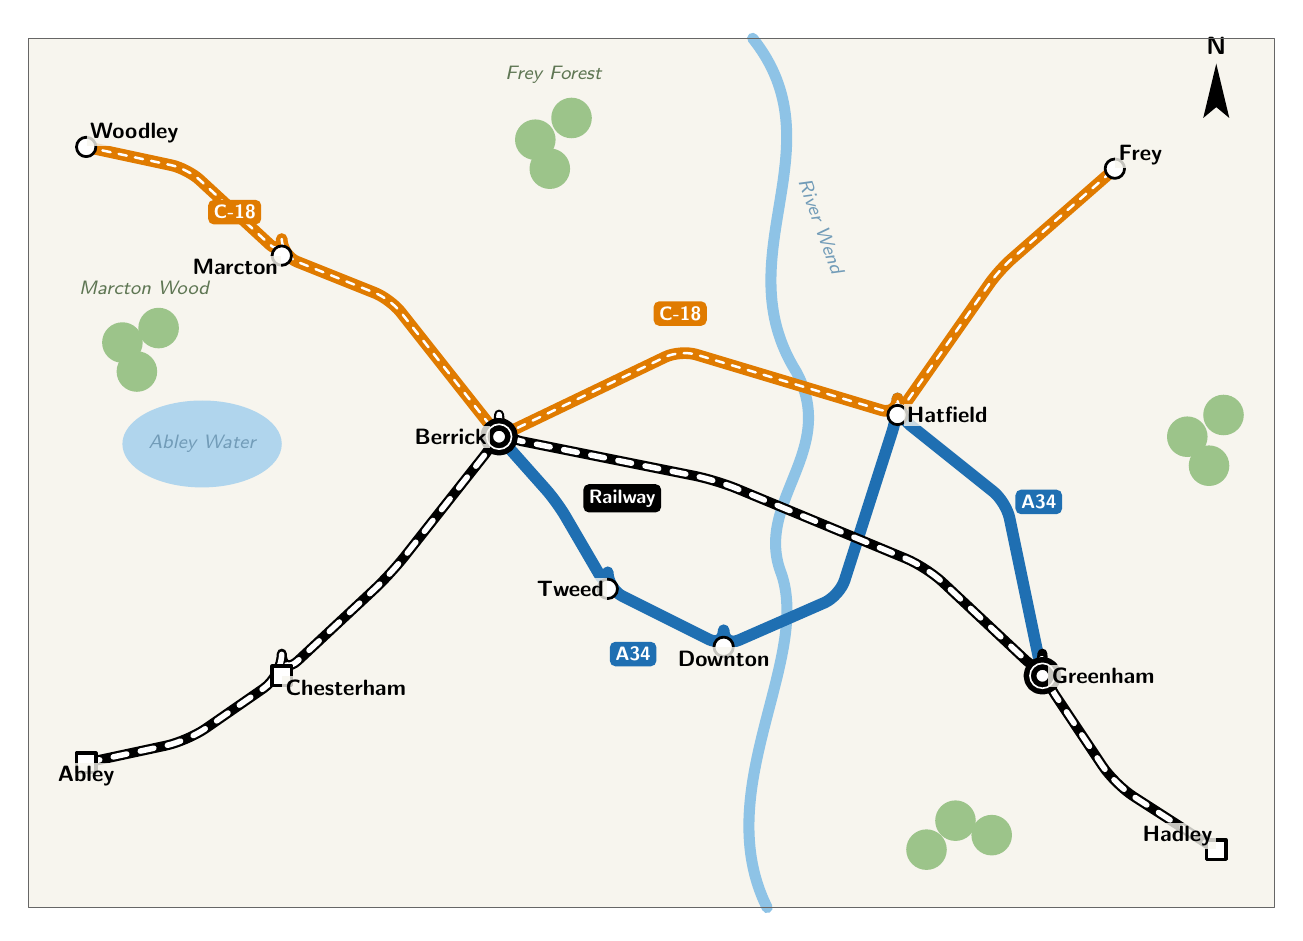
\begin{tikzpicture}[scale=0.92, line cap=round, line join=round]
\fill[mapbg] (0,0) rectangle (17.2,12);
\draw[river, line width=4.0pt] (10.0,12) .. controls (11.2,10.5) and (9.6,9.0) .. (10.6,7.4) .. controls (11.2,6.3) and (10.0,5.6) .. (10.4,4.6) .. controls (10.8,3.4) and (9.4,1.6) .. (10.2,0);
\fill[lake] (2.4,6.4) ellipse (1.1 and 0.6);
\node[font=\scriptsize\itshape, text=riverblue!80!black] at (2.4,6.4) {Abley Water};
\node[font=\scriptsize\itshape, text=riverblue!80!black, rotate=-70] at (10.95,9.4) {River Wend};
\fill[tree] (1.3,7.8) circle (0.28);
\fill[tree] (1.8,8.0) circle (0.28);
\fill[tree] (1.5,7.4) circle (0.28);
\fill[tree] (12.8,1.2) circle (0.28);
\fill[tree] (13.3,1.0) circle (0.28);
\fill[tree] (12.4,0.8) circle (0.28);
\fill[tree] (16.0,6.5) circle (0.28);
\fill[tree] (16.5,6.8) circle (0.28);
\fill[tree] (16.3,6.1) circle (0.28);
\fill[tree] (7.0,10.6) circle (0.28);
\fill[tree] (7.5,10.9) circle (0.28);
\fill[tree] (7.2,10.2) circle (0.28);
\node[font=\scriptsize\itshape, text=tree!60!black] at (1.6,8.55) {Marcton Wood};
\node[font=\scriptsize\itshape, text=tree!60!black] at (7.25,11.5) {Frey Forest};
\draw[a34, line width=4.2pt, rounded corners=6pt] (6.50,6.50) -- (7.30,5.60) -- (8.00,4.40) -- (8.00,4.40) -- (9.60,3.60) -- (9.60,3.60) -- (11.20,4.30) -- (12.00,6.80) -- (12.00,6.80) -- (13.50,5.60) -- (14.00,3.20);
\draw[c18, line width=4.2pt, rounded corners=6pt] (0.80,10.50) -- (2.20,10.20) -- (3.50,9.00) -- (3.50,9.00) -- (5.00,8.40) -- (6.50,6.50) -- (6.50,6.50) -- (9.00,7.70) -- (12.00,6.80) -- (12.00,6.80) -- (13.40,8.80) -- (15.00,10.20);
\draw[white, line width=0.9pt, dash pattern=on 3pt off 3pt, rounded corners=6pt] (0.80,10.50) -- (2.20,10.20) -- (3.50,9.00) -- (3.50,9.00) -- (5.00,8.40) -- (6.50,6.50) -- (6.50,6.50) -- (9.00,7.70) -- (12.00,6.80) -- (12.00,6.80) -- (13.40,8.80) -- (15.00,10.20);
\draw[black, line width=3.6pt, rounded corners=8pt] (0.80,2.00) -- (2.20,2.30) -- (3.50,3.20) -- (3.50,3.20) -- (5.00,4.60) -- (6.50,6.50) -- (6.50,6.50) -- (9.50,5.90) -- (12.40,4.70) -- (14.00,3.20) -- (14.00,3.20) -- (15.00,1.70) -- (16.40,0.80);
\draw[white, line width=2.0pt, dash pattern=on 5pt off 5pt, rounded corners=8pt] (0.80,2.00) -- (2.20,2.30) -- (3.50,3.20) -- (3.50,3.20) -- (5.00,4.60) -- (6.50,6.50) -- (6.50,6.50) -- (9.50,5.90) -- (12.40,4.70) -- (14.00,3.20) -- (14.00,3.20) -- (15.00,1.70) -- (16.40,0.80);
\node[badge=a34] at (8.35,3.5) {A34};
\node[badge=a34] at (13.95,5.6) {A34};
\node[badge=c18] at (9.0,8.2) {C-18};
\node[badge=c18] at (2.85,9.6) {C-18};
\node[badge=black] at (8.2,5.65) {Railway};
\begin{scope}[shift={(16.4,10.9)}]\fill[black] (0,0.75) -- (0.18,0) -- (0,0.15) -- (-0.18,0) -- cycle; \node[font=\bfseries\small] at (0,1.0) {N};\end{scope}
\node[busstop, minimum size=7.0pt] at (0.8,10.5) {};
\node[above right, font=\footnotesize\bfseries, fill=mapbg, fill opacity=0.8, text opacity=1, inner sep=1.2pt] at (0.8,10.5) {Woodley};
\node[busstop, minimum size=7.0pt] at (3.5,9.0) {};
\node[below left, font=\footnotesize\bfseries, fill=mapbg, fill opacity=0.8, text opacity=1, inner sep=1.2pt] at (3.5,9.0) {Marcton};
\node[inter, minimum size=9.0pt] at (6.5,6.5) {};
\node[left=3pt, font=\footnotesize\bfseries, fill=mapbg, fill opacity=0.8, text opacity=1, inner sep=1.2pt] at (6.5,6.5) {Berrick};
\node[busstop, minimum size=7.0pt] at (8.0,4.4) {};
\node[left, font=\footnotesize\bfseries, fill=mapbg, fill opacity=0.8, text opacity=1, inner sep=1.2pt] at (8.0,4.4) {Tweed};
\node[busstop, minimum size=7.0pt] at (9.6,3.6) {};
\node[below, font=\footnotesize\bfseries, fill=mapbg, fill opacity=0.8, text opacity=1, inner sep=1.2pt] at (9.6,3.6) {Downton};
\node[busstop, minimum size=7.0pt] at (12.0,6.8) {};
\node[right=2pt, font=\footnotesize\bfseries, fill=mapbg, fill opacity=0.8, text opacity=1, inner sep=1.2pt] at (12.0,6.8) {Hatfield};
\node[inter, minimum size=9.0pt] at (14.0,3.2) {};
\node[right=2pt, font=\footnotesize\bfseries, fill=mapbg, fill opacity=0.8, text opacity=1, inner sep=1.2pt] at (14.0,3.2) {Greenham};
\node[busstop, minimum size=7.0pt] at (15.0,10.2) {};
\node[above right, font=\footnotesize\bfseries, fill=mapbg, fill opacity=0.8, text opacity=1, inner sep=1.2pt] at (15.0,10.2) {Frey};
\node[station, minimum size=7.0pt] at (0.8,2.0) {};
\node[below, font=\footnotesize\bfseries, fill=mapbg, fill opacity=0.8, text opacity=1, inner sep=1.2pt] at (0.8,2.0) {Abley};
\node[station, minimum size=7.0pt] at (3.5,3.2) {};
\node[below right, font=\footnotesize\bfseries, fill=mapbg, fill opacity=0.8, text opacity=1, inner sep=1.2pt] at (3.5,3.2) {Chesterham};
\node[station, minimum size=7.0pt] at (16.4,0.8) {};
\node[above left, font=\footnotesize\bfseries, fill=mapbg, fill opacity=0.8, text opacity=1, inner sep=1.2pt] at (16.4,0.8) {Hadley};
\draw[black!60] (0,0) rectangle (17.2,12);
\end{tikzpicture}\end{center}\vspace{4pt}
{\small\begin{tabularx}{\linewidth}{p{4.9cm}|X|p{2.6cm}|p{2.6cm}}
\textbf{Vehicle} & \textbf{Not started / moving / finished?} & \textbf{Last stop} & \textbf{Next stop}\\\hline
& & & \\[5pt]\hline
& & & \\[5pt]\hline
& & & \\[5pt]\hline
& & & \\[5pt]\hline
& & & \\[5pt]\hline
& & & \\[5pt]\hline
& & & \\[5pt]\hline
& & & \\[5pt]\hline
& & & \\[5pt]\hline
& & & \\[5pt]\hline
& & & \\[5pt]\hline
& & & \\[5pt]\hline\end{tabularx}}
\clearpage
\banner{black!80}{Part B \quad Zoom in!}\par\smallskip
{\small Each picture zooms in on one route and is drawn \textbf{to scale by time}: every small mark on the line is \textbf{1 minute} of travel
(bigger marks every 5 minutes after a stop). The clock shows the moment the picture was frozen. The vehicles have been drawn for you.}\par\medskip

\banner{a34}{Zoom 1 \quad The A34 at 09:27}\par\smallskip\noindent\begin{minipage}[c]{0.13\linewidth}\centering 
\begin{tikzpicture}[baseline=-3pt]\draw[thick, fill=white] (0,0) circle (0.6);\draw[thick] (0.000,0.460) -- (0.000,0.600);\draw[] (0.265,0.459) -- (0.300,0.520);\draw[] (0.459,0.265) -- (0.520,0.300);\draw[thick] (0.460,0.000) -- (0.600,0.000);\draw[] (0.459,-0.265) -- (0.520,-0.300);\draw[] (0.265,-0.459) -- (0.300,-0.520);\draw[thick] (0.000,-0.460) -- (0.000,-0.600);\draw[] (-0.265,-0.459) -- (-0.300,-0.520);\draw[] (-0.459,-0.265) -- (-0.520,-0.300);\draw[thick] (-0.460,-0.000) -- (-0.600,-0.000);\draw[] (-0.459,0.265) -- (-0.520,0.300);\draw[] (-0.265,0.459) -- (-0.300,0.520);\draw[line width=1.4pt] (0,0) -- (-0.321,0.077);\draw[line width=0.8pt] (0,0) -- (0.158,-0.485);\fill (0,0) circle (1.2pt);\end{tikzpicture}\\{\bfseries 09:27}\end{minipage}\hfill\begin{minipage}[c]{0.86\linewidth}\centering 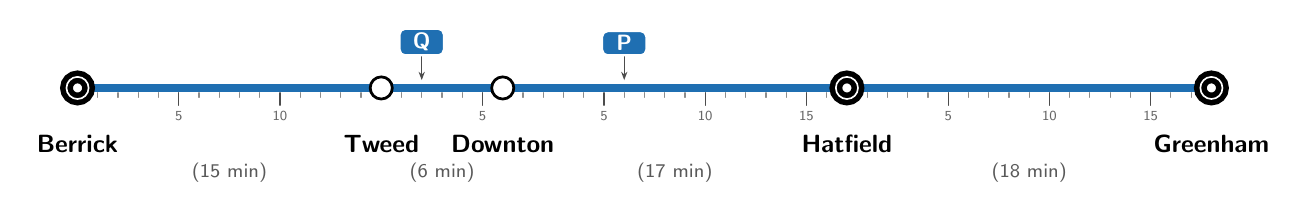
\begin{tikzpicture}[line cap=round]
\draw[a34, line width=3.2pt] (0,0) -- (14.40,0);
\draw[black!45] (0.257,-0.12) -- (0.257,-0.06);
\draw[black!45] (0.514,-0.12) -- (0.514,-0.06);
\draw[black!45] (0.771,-0.12) -- (0.771,-0.06);
\draw[black!45] (1.029,-0.12) -- (1.029,-0.06);
\draw[black!70] (1.286,-0.22) -- (1.286,-0.06);
\node[font=\tiny, text=black!60] at (1.286,-0.36) {5};
\draw[black!45] (1.543,-0.12) -- (1.543,-0.06);
\draw[black!45] (1.800,-0.12) -- (1.800,-0.06);
\draw[black!45] (2.057,-0.12) -- (2.057,-0.06);
\draw[black!45] (2.314,-0.12) -- (2.314,-0.06);
\draw[black!70] (2.571,-0.22) -- (2.571,-0.06);
\node[font=\tiny, text=black!60] at (2.571,-0.36) {10};
\draw[black!45] (2.829,-0.12) -- (2.829,-0.06);
\draw[black!45] (3.086,-0.12) -- (3.086,-0.06);
\draw[black!45] (3.343,-0.12) -- (3.343,-0.06);
\draw[black!45] (3.600,-0.12) -- (3.600,-0.06);
\draw[black!45] (4.114,-0.12) -- (4.114,-0.06);
\draw[black!45] (4.371,-0.12) -- (4.371,-0.06);
\draw[black!45] (4.629,-0.12) -- (4.629,-0.06);
\draw[black!45] (4.886,-0.12) -- (4.886,-0.06);
\draw[black!70] (5.143,-0.22) -- (5.143,-0.06);
\node[font=\tiny, text=black!60] at (5.143,-0.36) {5};
\draw[black!45] (5.657,-0.12) -- (5.657,-0.06);
\draw[black!45] (5.914,-0.12) -- (5.914,-0.06);
\draw[black!45] (6.171,-0.12) -- (6.171,-0.06);
\draw[black!45] (6.429,-0.12) -- (6.429,-0.06);
\draw[black!70] (6.686,-0.22) -- (6.686,-0.06);
\node[font=\tiny, text=black!60] at (6.686,-0.36) {5};
\draw[black!45] (6.943,-0.12) -- (6.943,-0.06);
\draw[black!45] (7.200,-0.12) -- (7.200,-0.06);
\draw[black!45] (7.457,-0.12) -- (7.457,-0.06);
\draw[black!45] (7.714,-0.12) -- (7.714,-0.06);
\draw[black!70] (7.971,-0.22) -- (7.971,-0.06);
\node[font=\tiny, text=black!60] at (7.971,-0.36) {10};
\draw[black!45] (8.229,-0.12) -- (8.229,-0.06);
\draw[black!45] (8.486,-0.12) -- (8.486,-0.06);
\draw[black!45] (8.743,-0.12) -- (8.743,-0.06);
\draw[black!45] (9.000,-0.12) -- (9.000,-0.06);
\draw[black!70] (9.257,-0.22) -- (9.257,-0.06);
\node[font=\tiny, text=black!60] at (9.257,-0.36) {15};
\draw[black!45] (9.514,-0.12) -- (9.514,-0.06);
\draw[black!45] (10.029,-0.12) -- (10.029,-0.06);
\draw[black!45] (10.286,-0.12) -- (10.286,-0.06);
\draw[black!45] (10.543,-0.12) -- (10.543,-0.06);
\draw[black!45] (10.800,-0.12) -- (10.800,-0.06);
\draw[black!70] (11.057,-0.22) -- (11.057,-0.06);
\node[font=\tiny, text=black!60] at (11.057,-0.36) {5};
\draw[black!45] (11.314,-0.12) -- (11.314,-0.06);
\draw[black!45] (11.571,-0.12) -- (11.571,-0.06);
\draw[black!45] (11.829,-0.12) -- (11.829,-0.06);
\draw[black!45] (12.086,-0.12) -- (12.086,-0.06);
\draw[black!70] (12.343,-0.22) -- (12.343,-0.06);
\node[font=\tiny, text=black!60] at (12.343,-0.36) {10};
\draw[black!45] (12.600,-0.12) -- (12.600,-0.06);
\draw[black!45] (12.857,-0.12) -- (12.857,-0.06);
\draw[black!45] (13.114,-0.12) -- (13.114,-0.06);
\draw[black!45] (13.371,-0.12) -- (13.371,-0.06);
\draw[black!70] (13.629,-0.22) -- (13.629,-0.06);
\node[font=\tiny, text=black!60] at (13.629,-0.36) {15};
\draw[black!45] (13.886,-0.12) -- (13.886,-0.06);
\draw[black!45] (14.143,-0.12) -- (14.143,-0.06);
\node[inter, minimum size=8pt] at (0.000,0) {};
\node[font=\small\bfseries, anchor=north] at (0.000,-0.48) {Berrick};
\node[busstop, minimum size=8pt] at (3.857,0) {};
\node[font=\small\bfseries, anchor=north] at (3.857,-0.48) {Tweed};
\node[busstop, minimum size=8pt] at (5.400,0) {};
\node[font=\small\bfseries, anchor=north] at (5.400,-0.48) {Downton};
\node[inter, minimum size=8pt] at (9.771,0) {};
\node[font=\small\bfseries, anchor=north] at (9.771,-0.48) {Hatfield};
\node[inter, minimum size=8pt] at (14.400,0) {};
\node[font=\small\bfseries, anchor=north] at (14.400,-0.48) {Greenham};
\node[font=\scriptsize, text=black!65] at (1.929,-1.08) {(15 min)};
\node[font=\scriptsize, text=black!65] at (4.629,-1.08) {(6 min)};
\node[font=\scriptsize, text=black!65] at (7.586,-1.08) {(17 min)};
\node[font=\scriptsize, text=black!65] at (12.086,-1.08) {(18 min)};
\draw[black!70, -{Stealth[length=3pt]}] (6.943,0.42) -- (6.943,0.1);
\node[busA, font=\footnotesize\bfseries, minimum width=16pt, above] at (6.943,0.4) {P};
\draw[black!70, -{Stealth[length=3pt]}] (4.371,0.42) -- (4.371,0.1);
\node[busA, font=\footnotesize\bfseries, minimum width=16pt, above] at (4.371,0.4) {Q};
\end{tikzpicture}\end{minipage}\par{\small \begin{enumerate}[label=\textbf{\alph*)}, leftmargin=*, itemsep=3pt, topsep=3pt]
\item Which bus is \textbf{P}, and which is \textbf{Q}? (Give the time each one left Berrick.) \hfill P: \aline\ \ Q: \aline
\item How many minutes until bus P reaches \textbf{Hatfield}? \aline\quad \textbf{Greenham}? \aline
\item How many minutes until bus Q reaches \textbf{Downton}? \aline\quad \textbf{Greenham}? \aline
\item Mark with a cross ($\times$) where bus P will be at \textbf{09:45}.
\item Tom arrives at the Tweed stop at 09:27, just as bus Q pulls away. How long must he wait for the next A34? \aline
\end{enumerate}}

\vspace{6pt}
\banner{c18}{Zoom 2 \quad The C-18 road at 10:05}\par\smallskip\noindent\begin{minipage}[c]{0.13\linewidth}\centering 
\begin{tikzpicture}[baseline=-3pt]\draw[thick, fill=white] (0,0) circle (0.6);\draw[thick] (0.000,0.460) -- (0.000,0.600);\draw[] (0.265,0.459) -- (0.300,0.520);\draw[] (0.459,0.265) -- (0.520,0.300);\draw[thick] (0.460,0.000) -- (0.600,0.000);\draw[] (0.459,-0.265) -- (0.520,-0.300);\draw[] (0.265,-0.459) -- (0.300,-0.520);\draw[thick] (0.000,-0.460) -- (0.000,-0.600);\draw[] (-0.265,-0.459) -- (-0.300,-0.520);\draw[] (-0.459,-0.265) -- (-0.520,-0.300);\draw[thick] (-0.460,-0.000) -- (-0.600,-0.000);\draw[] (-0.459,0.265) -- (-0.520,0.300);\draw[] (-0.265,0.459) -- (-0.300,0.520);\draw[line width=1.4pt] (0,0) -- (-0.278,0.177);\draw[line width=0.8pt] (0,0) -- (0.255,0.442);\fill (0,0) circle (1.2pt);\end{tikzpicture}\\{\bfseries 10:05}\end{minipage}\hfill\begin{minipage}[c]{0.86\linewidth}\centering 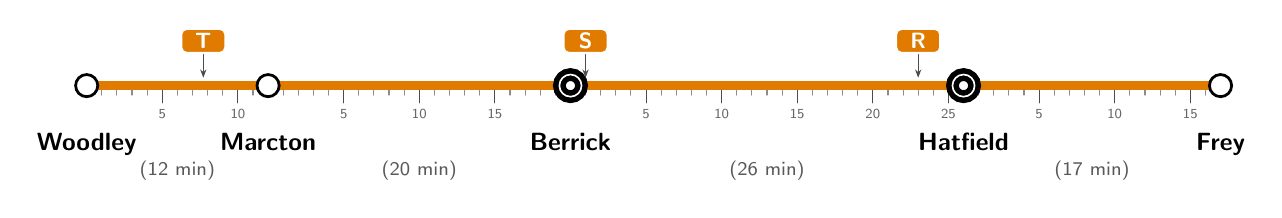
\begin{tikzpicture}[line cap=round]
\draw[c18, line width=3.2pt] (0,0) -- (14.40,0);
\draw[black!45] (0.192,-0.12) -- (0.192,-0.06);
\draw[black!45] (0.384,-0.12) -- (0.384,-0.06);
\draw[black!45] (0.576,-0.12) -- (0.576,-0.06);
\draw[black!45] (0.768,-0.12) -- (0.768,-0.06);
\draw[black!70] (0.960,-0.22) -- (0.960,-0.06);
\node[font=\tiny, text=black!60] at (0.960,-0.36) {5};
\draw[black!45] (1.152,-0.12) -- (1.152,-0.06);
\draw[black!45] (1.344,-0.12) -- (1.344,-0.06);
\draw[black!45] (1.536,-0.12) -- (1.536,-0.06);
\draw[black!45] (1.728,-0.12) -- (1.728,-0.06);
\draw[black!70] (1.920,-0.22) -- (1.920,-0.06);
\node[font=\tiny, text=black!60] at (1.920,-0.36) {10};
\draw[black!45] (2.112,-0.12) -- (2.112,-0.06);
\draw[black!45] (2.496,-0.12) -- (2.496,-0.06);
\draw[black!45] (2.688,-0.12) -- (2.688,-0.06);
\draw[black!45] (2.880,-0.12) -- (2.880,-0.06);
\draw[black!45] (3.072,-0.12) -- (3.072,-0.06);
\draw[black!70] (3.264,-0.22) -- (3.264,-0.06);
\node[font=\tiny, text=black!60] at (3.264,-0.36) {5};
\draw[black!45] (3.456,-0.12) -- (3.456,-0.06);
\draw[black!45] (3.648,-0.12) -- (3.648,-0.06);
\draw[black!45] (3.840,-0.12) -- (3.840,-0.06);
\draw[black!45] (4.032,-0.12) -- (4.032,-0.06);
\draw[black!70] (4.224,-0.22) -- (4.224,-0.06);
\node[font=\tiny, text=black!60] at (4.224,-0.36) {10};
\draw[black!45] (4.416,-0.12) -- (4.416,-0.06);
\draw[black!45] (4.608,-0.12) -- (4.608,-0.06);
\draw[black!45] (4.800,-0.12) -- (4.800,-0.06);
\draw[black!45] (4.992,-0.12) -- (4.992,-0.06);
\draw[black!70] (5.184,-0.22) -- (5.184,-0.06);
\node[font=\tiny, text=black!60] at (5.184,-0.36) {15};
\draw[black!45] (5.376,-0.12) -- (5.376,-0.06);
\draw[black!45] (5.568,-0.12) -- (5.568,-0.06);
\draw[black!45] (5.760,-0.12) -- (5.760,-0.06);
\draw[black!45] (5.952,-0.12) -- (5.952,-0.06);
\draw[black!45] (6.336,-0.12) -- (6.336,-0.06);
\draw[black!45] (6.528,-0.12) -- (6.528,-0.06);
\draw[black!45] (6.720,-0.12) -- (6.720,-0.06);
\draw[black!45] (6.912,-0.12) -- (6.912,-0.06);
\draw[black!70] (7.104,-0.22) -- (7.104,-0.06);
\node[font=\tiny, text=black!60] at (7.104,-0.36) {5};
\draw[black!45] (7.296,-0.12) -- (7.296,-0.06);
\draw[black!45] (7.488,-0.12) -- (7.488,-0.06);
\draw[black!45] (7.680,-0.12) -- (7.680,-0.06);
\draw[black!45] (7.872,-0.12) -- (7.872,-0.06);
\draw[black!70] (8.064,-0.22) -- (8.064,-0.06);
\node[font=\tiny, text=black!60] at (8.064,-0.36) {10};
\draw[black!45] (8.256,-0.12) -- (8.256,-0.06);
\draw[black!45] (8.448,-0.12) -- (8.448,-0.06);
\draw[black!45] (8.640,-0.12) -- (8.640,-0.06);
\draw[black!45] (8.832,-0.12) -- (8.832,-0.06);
\draw[black!70] (9.024,-0.22) -- (9.024,-0.06);
\node[font=\tiny, text=black!60] at (9.024,-0.36) {15};
\draw[black!45] (9.216,-0.12) -- (9.216,-0.06);
\draw[black!45] (9.408,-0.12) -- (9.408,-0.06);
\draw[black!45] (9.600,-0.12) -- (9.600,-0.06);
\draw[black!45] (9.792,-0.12) -- (9.792,-0.06);
\draw[black!70] (9.984,-0.22) -- (9.984,-0.06);
\node[font=\tiny, text=black!60] at (9.984,-0.36) {20};
\draw[black!45] (10.176,-0.12) -- (10.176,-0.06);
\draw[black!45] (10.368,-0.12) -- (10.368,-0.06);
\draw[black!45] (10.560,-0.12) -- (10.560,-0.06);
\draw[black!45] (10.752,-0.12) -- (10.752,-0.06);
\draw[black!70] (10.944,-0.22) -- (10.944,-0.06);
\node[font=\tiny, text=black!60] at (10.944,-0.36) {25};
\draw[black!45] (11.328,-0.12) -- (11.328,-0.06);
\draw[black!45] (11.520,-0.12) -- (11.520,-0.06);
\draw[black!45] (11.712,-0.12) -- (11.712,-0.06);
\draw[black!45] (11.904,-0.12) -- (11.904,-0.06);
\draw[black!70] (12.096,-0.22) -- (12.096,-0.06);
\node[font=\tiny, text=black!60] at (12.096,-0.36) {5};
\draw[black!45] (12.288,-0.12) -- (12.288,-0.06);
\draw[black!45] (12.480,-0.12) -- (12.480,-0.06);
\draw[black!45] (12.672,-0.12) -- (12.672,-0.06);
\draw[black!45] (12.864,-0.12) -- (12.864,-0.06);
\draw[black!70] (13.056,-0.22) -- (13.056,-0.06);
\node[font=\tiny, text=black!60] at (13.056,-0.36) {10};
\draw[black!45] (13.248,-0.12) -- (13.248,-0.06);
\draw[black!45] (13.440,-0.12) -- (13.440,-0.06);
\draw[black!45] (13.632,-0.12) -- (13.632,-0.06);
\draw[black!45] (13.824,-0.12) -- (13.824,-0.06);
\draw[black!70] (14.016,-0.22) -- (14.016,-0.06);
\node[font=\tiny, text=black!60] at (14.016,-0.36) {15};
\draw[black!45] (14.208,-0.12) -- (14.208,-0.06);
\node[busstop, minimum size=8pt] at (0.000,0) {};
\node[font=\small\bfseries, anchor=north] at (0.000,-0.48) {Woodley};
\node[busstop, minimum size=8pt] at (2.304,0) {};
\node[font=\small\bfseries, anchor=north] at (2.304,-0.48) {Marcton};
\node[inter, minimum size=8pt] at (6.144,0) {};
\node[font=\small\bfseries, anchor=north] at (6.144,-0.48) {Berrick};
\node[inter, minimum size=8pt] at (11.136,0) {};
\node[font=\small\bfseries, anchor=north] at (11.136,-0.48) {Hatfield};
\node[busstop, minimum size=8pt] at (14.400,0) {};
\node[font=\small\bfseries, anchor=north] at (14.400,-0.48) {Frey};
\node[font=\scriptsize, text=black!65] at (1.152,-1.08) {(12 min)};
\node[font=\scriptsize, text=black!65] at (4.224,-1.08) {(20 min)};
\node[font=\scriptsize, text=black!65] at (8.640,-1.08) {(26 min)};
\node[font=\scriptsize, text=black!65] at (12.768,-1.08) {(17 min)};
\draw[black!70, -{Stealth[length=3pt]}] (10.560,0.42) -- (10.560,0.1);
\node[busC, font=\footnotesize\bfseries, minimum width=16pt, above] at (10.560,0.4) {R};
\draw[black!70, -{Stealth[length=3pt]}] (6.336,0.42) -- (6.336,0.1);
\node[busC, font=\footnotesize\bfseries, minimum width=16pt, above] at (6.336,0.4) {S};
\draw[black!70, -{Stealth[length=3pt]}] (1.481,0.42) -- (1.481,0.1);
\node[busC, font=\footnotesize\bfseries, minimum width=16pt, above] at (1.481,0.4) {T};
\end{tikzpicture}\end{minipage}\par{\small \begin{enumerate}[label=\textbf{\alph*)}, leftmargin=*, itemsep=3pt, topsep=3pt]
\item Which bus is \textbf{R}, \textbf{S} and \textbf{T}? (C-18, C-18A or C-18B?) \\[3pt] R: \sline\quad S: \sline\quad T: \sline
\item How many minutes until each bus reaches \textbf{Frey}? \\[3pt] R: \sline\quad S: \sline\quad T: \sline
\item Bus S has only just gone past Berrick. Why couldn't Karen, who was waiting at Berrick, get on it?
\item Karen is still at Berrick at 10:05 and wants to get to Frey. When is the next C-18 she can catch? How long will she wait?\\[3pt] \aline\aline
\item Mark with a cross ($\times$) where bus R will be at \textbf{10:15}.
\end{enumerate}}

\vspace{6pt}
\banner{black!85}{Zoom 3 \quad The railway at 10:10}\par\smallskip\noindent\begin{minipage}[c]{0.13\linewidth}\centering 
\begin{tikzpicture}[baseline=-3pt]\draw[thick, fill=white] (0,0) circle (0.6);\draw[thick] (0.000,0.460) -- (0.000,0.600);\draw[] (0.265,0.459) -- (0.300,0.520);\draw[] (0.459,0.265) -- (0.520,0.300);\draw[thick] (0.460,0.000) -- (0.600,0.000);\draw[] (0.459,-0.265) -- (0.520,-0.300);\draw[] (0.265,-0.459) -- (0.300,-0.520);\draw[thick] (0.000,-0.460) -- (0.000,-0.600);\draw[] (-0.265,-0.459) -- (-0.300,-0.520);\draw[] (-0.459,-0.265) -- (-0.520,-0.300);\draw[thick] (-0.460,-0.000) -- (-0.600,-0.000);\draw[] (-0.459,0.265) -- (-0.520,0.300);\draw[] (-0.265,0.459) -- (-0.300,0.520);\draw[line width=1.4pt] (0,0) -- (-0.270,0.189);\draw[line width=0.8pt] (0,0) -- (0.442,0.255);\fill (0,0) circle (1.2pt);\end{tikzpicture}\\{\bfseries 10:10}\end{minipage}\hfill\begin{minipage}[c]{0.86\linewidth}\centering 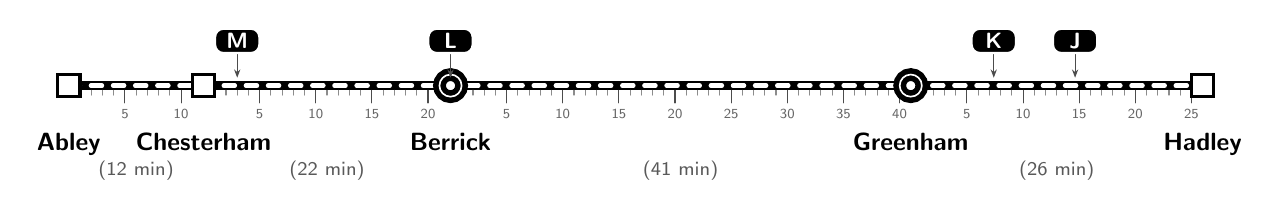
\begin{tikzpicture}[line cap=round]
\draw[black, line width=3pt] (0,0) -- (14.40,0);
\draw[white, line width=1.6pt, dash pattern=on 4pt off 4pt] (0,0) -- (14.40,0);
\draw[black!45] (0.143,-0.12) -- (0.143,-0.06);
\draw[black!45] (0.285,-0.12) -- (0.285,-0.06);
\draw[black!45] (0.428,-0.12) -- (0.428,-0.06);
\draw[black!45] (0.570,-0.12) -- (0.570,-0.06);
\draw[black!70] (0.713,-0.22) -- (0.713,-0.06);
\node[font=\tiny, text=black!60] at (0.713,-0.36) {5};
\draw[black!45] (0.855,-0.12) -- (0.855,-0.06);
\draw[black!45] (0.998,-0.12) -- (0.998,-0.06);
\draw[black!45] (1.141,-0.12) -- (1.141,-0.06);
\draw[black!45] (1.283,-0.12) -- (1.283,-0.06);
\draw[black!70] (1.426,-0.22) -- (1.426,-0.06);
\node[font=\tiny, text=black!60] at (1.426,-0.36) {10};
\draw[black!45] (1.568,-0.12) -- (1.568,-0.06);
\draw[black!45] (1.853,-0.12) -- (1.853,-0.06);
\draw[black!45] (1.996,-0.12) -- (1.996,-0.06);
\draw[black!45] (2.139,-0.12) -- (2.139,-0.06);
\draw[black!45] (2.281,-0.12) -- (2.281,-0.06);
\draw[black!70] (2.424,-0.22) -- (2.424,-0.06);
\node[font=\tiny, text=black!60] at (2.424,-0.36) {5};
\draw[black!45] (2.566,-0.12) -- (2.566,-0.06);
\draw[black!45] (2.709,-0.12) -- (2.709,-0.06);
\draw[black!45] (2.851,-0.12) -- (2.851,-0.06);
\draw[black!45] (2.994,-0.12) -- (2.994,-0.06);
\draw[black!70] (3.137,-0.22) -- (3.137,-0.06);
\node[font=\tiny, text=black!60] at (3.137,-0.36) {10};
\draw[black!45] (3.279,-0.12) -- (3.279,-0.06);
\draw[black!45] (3.422,-0.12) -- (3.422,-0.06);
\draw[black!45] (3.564,-0.12) -- (3.564,-0.06);
\draw[black!45] (3.707,-0.12) -- (3.707,-0.06);
\draw[black!70] (3.850,-0.22) -- (3.850,-0.06);
\node[font=\tiny, text=black!60] at (3.850,-0.36) {15};
\draw[black!45] (3.992,-0.12) -- (3.992,-0.06);
\draw[black!45] (4.135,-0.12) -- (4.135,-0.06);
\draw[black!45] (4.277,-0.12) -- (4.277,-0.06);
\draw[black!45] (4.420,-0.12) -- (4.420,-0.06);
\draw[black!70] (4.562,-0.22) -- (4.562,-0.06);
\node[font=\tiny, text=black!60] at (4.562,-0.36) {20};
\draw[black!45] (4.705,-0.12) -- (4.705,-0.06);
\draw[black!45] (4.990,-0.12) -- (4.990,-0.06);
\draw[black!45] (5.133,-0.12) -- (5.133,-0.06);
\draw[black!45] (5.275,-0.12) -- (5.275,-0.06);
\draw[black!45] (5.418,-0.12) -- (5.418,-0.06);
\draw[black!70] (5.560,-0.22) -- (5.560,-0.06);
\node[font=\tiny, text=black!60] at (5.560,-0.36) {5};
\draw[black!45] (5.703,-0.12) -- (5.703,-0.06);
\draw[black!45] (5.846,-0.12) -- (5.846,-0.06);
\draw[black!45] (5.988,-0.12) -- (5.988,-0.06);
\draw[black!45] (6.131,-0.12) -- (6.131,-0.06);
\draw[black!70] (6.273,-0.22) -- (6.273,-0.06);
\node[font=\tiny, text=black!60] at (6.273,-0.36) {10};
\draw[black!45] (6.416,-0.12) -- (6.416,-0.06);
\draw[black!45] (6.558,-0.12) -- (6.558,-0.06);
\draw[black!45] (6.701,-0.12) -- (6.701,-0.06);
\draw[black!45] (6.844,-0.12) -- (6.844,-0.06);
\draw[black!70] (6.986,-0.22) -- (6.986,-0.06);
\node[font=\tiny, text=black!60] at (6.986,-0.36) {15};
\draw[black!45] (7.129,-0.12) -- (7.129,-0.06);
\draw[black!45] (7.271,-0.12) -- (7.271,-0.06);
\draw[black!45] (7.414,-0.12) -- (7.414,-0.06);
\draw[black!45] (7.556,-0.12) -- (7.556,-0.06);
\draw[black!70] (7.699,-0.22) -- (7.699,-0.06);
\node[font=\tiny, text=black!60] at (7.699,-0.36) {20};
\draw[black!45] (7.842,-0.12) -- (7.842,-0.06);
\draw[black!45] (7.984,-0.12) -- (7.984,-0.06);
\draw[black!45] (8.127,-0.12) -- (8.127,-0.06);
\draw[black!45] (8.269,-0.12) -- (8.269,-0.06);
\draw[black!70] (8.412,-0.22) -- (8.412,-0.06);
\node[font=\tiny, text=black!60] at (8.412,-0.36) {25};
\draw[black!45] (8.554,-0.12) -- (8.554,-0.06);
\draw[black!45] (8.697,-0.12) -- (8.697,-0.06);
\draw[black!45] (8.840,-0.12) -- (8.840,-0.06);
\draw[black!45] (8.982,-0.12) -- (8.982,-0.06);
\draw[black!70] (9.125,-0.22) -- (9.125,-0.06);
\node[font=\tiny, text=black!60] at (9.125,-0.36) {30};
\draw[black!45] (9.267,-0.12) -- (9.267,-0.06);
\draw[black!45] (9.410,-0.12) -- (9.410,-0.06);
\draw[black!45] (9.552,-0.12) -- (9.552,-0.06);
\draw[black!45] (9.695,-0.12) -- (9.695,-0.06);
\draw[black!70] (9.838,-0.22) -- (9.838,-0.06);
\node[font=\tiny, text=black!60] at (9.838,-0.36) {35};
\draw[black!45] (9.980,-0.12) -- (9.980,-0.06);
\draw[black!45] (10.123,-0.12) -- (10.123,-0.06);
\draw[black!45] (10.265,-0.12) -- (10.265,-0.06);
\draw[black!45] (10.408,-0.12) -- (10.408,-0.06);
\draw[black!70] (10.550,-0.22) -- (10.550,-0.06);
\node[font=\tiny, text=black!60] at (10.550,-0.36) {40};
\draw[black!45] (10.836,-0.12) -- (10.836,-0.06);
\draw[black!45] (10.978,-0.12) -- (10.978,-0.06);
\draw[black!45] (11.121,-0.12) -- (11.121,-0.06);
\draw[black!45] (11.263,-0.12) -- (11.263,-0.06);
\draw[black!70] (11.406,-0.22) -- (11.406,-0.06);
\node[font=\tiny, text=black!60] at (11.406,-0.36) {5};
\draw[black!45] (11.549,-0.12) -- (11.549,-0.06);
\draw[black!45] (11.691,-0.12) -- (11.691,-0.06);
\draw[black!45] (11.834,-0.12) -- (11.834,-0.06);
\draw[black!45] (11.976,-0.12) -- (11.976,-0.06);
\draw[black!70] (12.119,-0.22) -- (12.119,-0.06);
\node[font=\tiny, text=black!60] at (12.119,-0.36) {10};
\draw[black!45] (12.261,-0.12) -- (12.261,-0.06);
\draw[black!45] (12.404,-0.12) -- (12.404,-0.06);
\draw[black!45] (12.547,-0.12) -- (12.547,-0.06);
\draw[black!45] (12.689,-0.12) -- (12.689,-0.06);
\draw[black!70] (12.832,-0.22) -- (12.832,-0.06);
\node[font=\tiny, text=black!60] at (12.832,-0.36) {15};
\draw[black!45] (12.974,-0.12) -- (12.974,-0.06);
\draw[black!45] (13.117,-0.12) -- (13.117,-0.06);
\draw[black!45] (13.259,-0.12) -- (13.259,-0.06);
\draw[black!45] (13.402,-0.12) -- (13.402,-0.06);
\draw[black!70] (13.545,-0.22) -- (13.545,-0.06);
\node[font=\tiny, text=black!60] at (13.545,-0.36) {20};
\draw[black!45] (13.687,-0.12) -- (13.687,-0.06);
\draw[black!45] (13.830,-0.12) -- (13.830,-0.06);
\draw[black!45] (13.972,-0.12) -- (13.972,-0.06);
\draw[black!45] (14.115,-0.12) -- (14.115,-0.06);
\draw[black!70] (14.257,-0.22) -- (14.257,-0.06);
\node[font=\tiny, text=black!60] at (14.257,-0.36) {25};
\node[station, minimum size=8pt] at (0.000,0) {};
\node[font=\small\bfseries, anchor=north] at (0.000,-0.48) {Abley};
\node[station, minimum size=8pt] at (1.711,0) {};
\node[font=\small\bfseries, anchor=north] at (1.711,-0.48) {Chesterham};
\node[inter, minimum size=8pt] at (4.848,0) {};
\node[font=\small\bfseries, anchor=north] at (4.848,-0.48) {Berrick};
\node[inter, minimum size=8pt] at (10.693,0) {};
\node[font=\small\bfseries, anchor=north] at (10.693,-0.48) {Greenham};
\node[station, minimum size=8pt] at (14.400,0) {};
\node[font=\small\bfseries, anchor=north] at (14.400,-0.48) {Hadley};
\node[font=\scriptsize, text=black!65] at (0.855,-1.08) {(12 min)};
\node[font=\scriptsize, text=black!65] at (3.279,-1.08) {(22 min)};
\node[font=\scriptsize, text=black!65] at (7.770,-1.08) {(41 min)};
\node[font=\scriptsize, text=black!65] at (12.547,-1.08) {(26 min)};
\draw[black!70, -{Stealth[length=3pt]}] (12.780,0.42) -- (12.780,0.1);
\node[train, font=\footnotesize\bfseries, minimum width=16pt, above] at (12.780,0.4) {J};
\draw[black!70, -{Stealth[length=3pt]}] (11.747,0.42) -- (11.747,0.1);
\node[train, font=\footnotesize\bfseries, minimum width=16pt, above] at (11.747,0.4) {K};
\draw[black!70, -{Stealth[length=3pt]}] (4.848,0.42) -- (4.848,0.1);
\node[train, font=\footnotesize\bfseries, minimum width=16pt, above] at (4.848,0.4) {L};
\draw[black!70, -{Stealth[length=3pt]}] (2.139,0.42) -- (2.139,0.1);
\node[train, font=\footnotesize\bfseries, minimum width=16pt, above] at (2.139,0.4) {M};
\end{tikzpicture}\end{minipage}\par{\small \begin{enumerate}[label=\textbf{\alph*)}, leftmargin=*, itemsep=3pt, topsep=3pt]
\item Which train is \textbf{J}, \textbf{K}, \textbf{L} and \textbf{M}? (Give the time each left Abley.) \\[3pt] J: \sline\quad K: \sline\quad L: \sline\quad M: \sline
\item How many minutes until each train reaches \textbf{Hadley}? \\[3pt] J: \sline\quad K: \sline\quad L: \sline\quad M: \sline
\item Train J left Abley 15 minutes \emph{after} train K, but it is now \emph{in front}. How can you tell from the timetable that J must have overtaken K?
\item Priya gets to Greenham station at 10:10 and wants to go to Hadley. Train K is about to go past. When is the next train she can catch, and how long will she wait? \aline
\item Mark with a cross ($\times$) where train M will be at \textbf{10:20}.
\end{enumerate}}

\clearpage
\vspace{8pt}\banner{black!80}{Part C \quad Countdown boards}\par\smallskip{\small Real bus stops and stations show how many minutes until each service leaves. Fill in the boards.}\par\medskip\begin{center}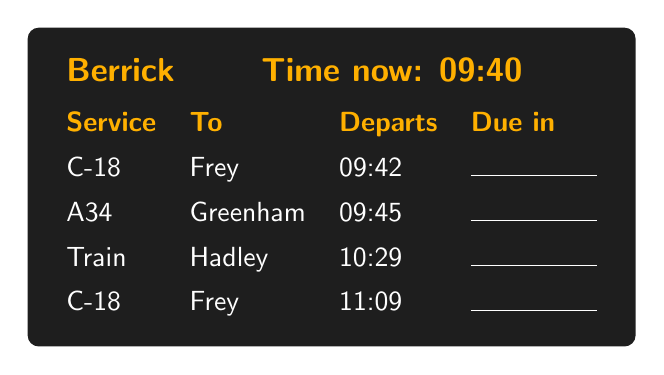
\begin{tikzpicture}\node[fill=board, rounded corners=4pt, inner sep=8pt]{\begin{tabular}{llll}\multicolumn{4}{l}{\textcolor{amber}{\bfseries\large Berrick \hfill Time now: 09:40}}\\[2pt]\textcolor{amber}{\bfseries Service} & \textcolor{amber}{\bfseries To} & \textcolor{amber}{\bfseries Departs} & \textcolor{amber}{\bfseries Due in}\\\textcolor{white}{C-18} & \textcolor{white}{Frey} & \textcolor{white}{09:42} & \textcolor{white}{\rule{1.6cm}{0.4pt}}\\
\textcolor{white}{A34} & \textcolor{white}{Greenham} & \textcolor{white}{09:45} & \textcolor{white}{\rule{1.6cm}{0.4pt}}\\
\textcolor{white}{Train} & \textcolor{white}{Hadley} & \textcolor{white}{10:29} & \textcolor{white}{\rule{1.6cm}{0.4pt}}\\
\textcolor{white}{C-18} & \textcolor{white}{Frey} & \textcolor{white}{11:09} & \textcolor{white}{\rule{1.6cm}{0.4pt}}\\\end{tabular}};\end{tikzpicture}\hspace{0.4cm}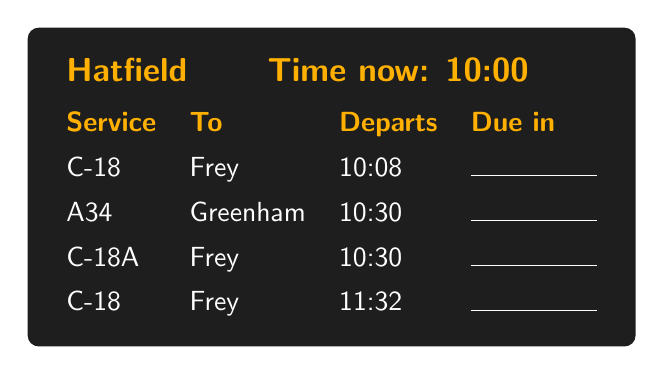
\begin{tikzpicture}\node[fill=board, rounded corners=4pt, inner sep=8pt]{\begin{tabular}{llll}\multicolumn{4}{l}{\textcolor{amber}{\bfseries\large Hatfield \hfill Time now: 10:00}}\\[2pt]\textcolor{amber}{\bfseries Service} & \textcolor{amber}{\bfseries To} & \textcolor{amber}{\bfseries Departs} & \textcolor{amber}{\bfseries Due in}\\\textcolor{white}{C-18} & \textcolor{white}{Frey} & \textcolor{white}{10:08} & \textcolor{white}{\rule{1.6cm}{0.4pt}}\\
\textcolor{white}{A34} & \textcolor{white}{Greenham} & \textcolor{white}{10:30} & \textcolor{white}{\rule{1.6cm}{0.4pt}}\\
\textcolor{white}{C-18A} & \textcolor{white}{Frey} & \textcolor{white}{10:30} & \textcolor{white}{\rule{1.6cm}{0.4pt}}\\
\textcolor{white}{C-18} & \textcolor{white}{Frey} & \textcolor{white}{11:32} & \textcolor{white}{\rule{1.6cm}{0.4pt}}\\\end{tabular}};\end{tikzpicture}\end{center}{\small \begin{enumerate}[label=\textbf{\alph*)}, leftmargin=*, itemsep=3pt, topsep=3pt]
\item Fill in the \textbf{Due in} column on both boards.
\item Lily is at Berrick at 09:40 and wants to get to \textbf{Hatfield}. Which service should she catch? What time will she arrive? \aline
\item At Hatfield at 10:00, you want to get to Frey. Which bus gets you there first? How long from now until you arrive? \aline
\item \textbf{Make your own:} choose a stop and a time, and write a departure board for a partner to fill in.
\end{enumerate}}
\clearpage\begin{center}{\LARGE\bfseries Answers}\end{center}\vspace{-4pt}
{\small Vehicle positions are drawn assuming steady speed between stops. For vehicles that go straight past a stop, the position is shared out over the whole non-stop stretch, so treat those as approximate.}\par\medskip
\noindent\begin{minipage}[t]{0.555\linewidth}\vspace{0pt}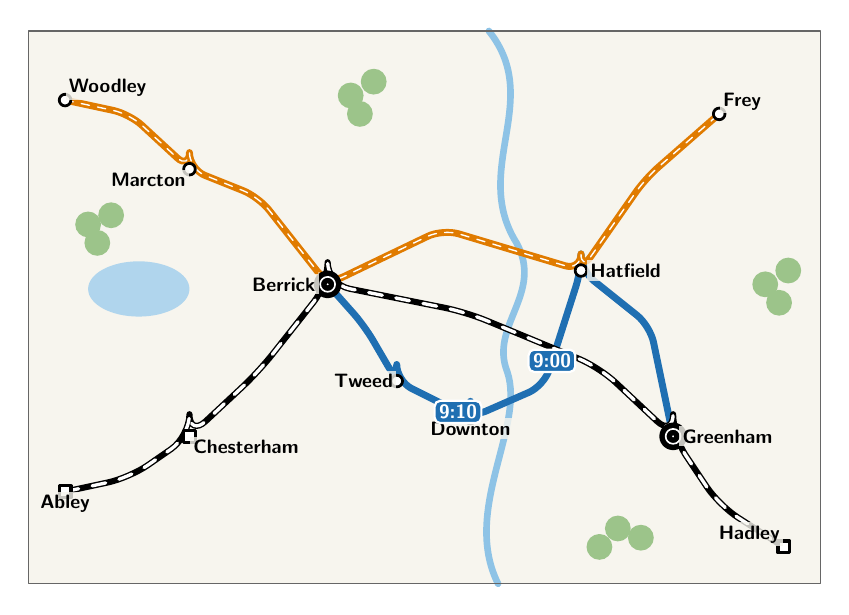
\begin{tikzpicture}[scale=0.585, line cap=round, line join=round]
\fill[mapbg] (0,0) rectangle (17.2,12);
\draw[river, line width=2.4pt] (10.0,12) .. controls (11.2,10.5) and (9.6,9.0) .. (10.6,7.4) .. controls (11.2,6.3) and (10.0,5.6) .. (10.4,4.6) .. controls (10.8,3.4) and (9.4,1.6) .. (10.2,0);
\fill[lake] (2.4,6.4) ellipse (1.1 and 0.6);
\fill[tree] (1.3,7.8) circle (0.28);
\fill[tree] (1.8,8.0) circle (0.28);
\fill[tree] (1.5,7.4) circle (0.28);
\fill[tree] (12.8,1.2) circle (0.28);
\fill[tree] (13.3,1.0) circle (0.28);
\fill[tree] (12.4,0.8) circle (0.28);
\fill[tree] (16.0,6.5) circle (0.28);
\fill[tree] (16.5,6.8) circle (0.28);
\fill[tree] (16.3,6.1) circle (0.28);
\fill[tree] (7.0,10.6) circle (0.28);
\fill[tree] (7.5,10.9) circle (0.28);
\fill[tree] (7.2,10.2) circle (0.28);
\draw[a34, line width=2.5pt, rounded corners=6pt] (6.50,6.50) -- (7.30,5.60) -- (8.00,4.40) -- (8.00,4.40) -- (9.60,3.60) -- (9.60,3.60) -- (11.20,4.30) -- (12.00,6.80) -- (12.00,6.80) -- (13.50,5.60) -- (14.00,3.20);
\draw[c18, line width=2.5pt, rounded corners=6pt] (0.80,10.50) -- (2.20,10.20) -- (3.50,9.00) -- (3.50,9.00) -- (5.00,8.40) -- (6.50,6.50) -- (6.50,6.50) -- (9.00,7.70) -- (12.00,6.80) -- (12.00,6.80) -- (13.40,8.80) -- (15.00,10.20);
\draw[white, line width=0.5pt, dash pattern=on 3pt off 3pt, rounded corners=6pt] (0.80,10.50) -- (2.20,10.20) -- (3.50,9.00) -- (3.50,9.00) -- (5.00,8.40) -- (6.50,6.50) -- (6.50,6.50) -- (9.00,7.70) -- (12.00,6.80) -- (12.00,6.80) -- (13.40,8.80) -- (15.00,10.20);
\draw[black, line width=2.2pt, rounded corners=8pt] (0.80,2.00) -- (2.20,2.30) -- (3.50,3.20) -- (3.50,3.20) -- (5.00,4.60) -- (6.50,6.50) -- (6.50,6.50) -- (9.50,5.90) -- (12.40,4.70) -- (14.00,3.20) -- (14.00,3.20) -- (15.00,1.70) -- (16.40,0.80);
\draw[white, line width=1.2pt, dash pattern=on 5pt off 5pt, rounded corners=8pt] (0.80,2.00) -- (2.20,2.30) -- (3.50,3.20) -- (3.50,3.20) -- (5.00,4.60) -- (6.50,6.50) -- (6.50,6.50) -- (9.50,5.90) -- (12.40,4.70) -- (14.00,3.20) -- (14.00,3.20) -- (15.00,1.70) -- (16.40,0.80);
\node[busstop, minimum size=4.2pt] at (0.8,10.5) {};
\node[above right, font=\scriptsize\bfseries, fill=mapbg, fill opacity=0.8, text opacity=1, inner sep=1.2pt] at (0.8,10.5) {Woodley};
\node[busstop, minimum size=4.2pt] at (3.5,9.0) {};
\node[below left, font=\scriptsize\bfseries, fill=mapbg, fill opacity=0.8, text opacity=1, inner sep=1.2pt] at (3.5,9.0) {Marcton};
\node[inter, minimum size=5.4pt] at (6.5,6.5) {};
\node[left=3pt, font=\scriptsize\bfseries, fill=mapbg, fill opacity=0.8, text opacity=1, inner sep=1.2pt] at (6.5,6.5) {Berrick};
\node[busstop, minimum size=4.2pt] at (8.0,4.4) {};
\node[left, font=\scriptsize\bfseries, fill=mapbg, fill opacity=0.8, text opacity=1, inner sep=1.2pt] at (8.0,4.4) {Tweed};
\node[busstop, minimum size=4.2pt] at (9.6,3.6) {};
\node[below, font=\scriptsize\bfseries, fill=mapbg, fill opacity=0.8, text opacity=1, inner sep=1.2pt] at (9.6,3.6) {Downton};
\node[busstop, minimum size=4.2pt] at (12.0,6.8) {};
\node[right=2pt, font=\scriptsize\bfseries, fill=mapbg, fill opacity=0.8, text opacity=1, inner sep=1.2pt] at (12.0,6.8) {Hatfield};
\node[inter, minimum size=5.4pt] at (14.0,3.2) {};
\node[right=2pt, font=\scriptsize\bfseries, fill=mapbg, fill opacity=0.8, text opacity=1, inner sep=1.2pt] at (14.0,3.2) {Greenham};
\node[busstop, minimum size=4.2pt] at (15.0,10.2) {};
\node[above right, font=\scriptsize\bfseries, fill=mapbg, fill opacity=0.8, text opacity=1, inner sep=1.2pt] at (15.0,10.2) {Frey};
\node[station, minimum size=4.2pt] at (0.8,2.0) {};
\node[below, font=\scriptsize\bfseries, fill=mapbg, fill opacity=0.8, text opacity=1, inner sep=1.2pt] at (0.8,2.0) {Abley};
\node[station, minimum size=4.2pt] at (3.5,3.2) {};
\node[below right, font=\scriptsize\bfseries, fill=mapbg, fill opacity=0.8, text opacity=1, inner sep=1.2pt] at (3.5,3.2) {Chesterham};
\node[station, minimum size=4.2pt] at (16.4,0.8) {};
\node[above left, font=\scriptsize\bfseries, fill=mapbg, fill opacity=0.8, text opacity=1, inner sep=1.2pt] at (16.4,0.8) {Hadley};
\node[busA] at (11.37,4.84) {9:00};
\node[busA] at (9.33,3.73) {9:10};
\draw[black!60] (0,0) rectangle (17.2,12);
\end{tikzpicture}\end{minipage}\hfill\begin{minipage}[t]{0.425\linewidth}\vspace{0pt}{\large\bfseries 1.}\ \ 
\begin{tikzpicture}[baseline=-3pt]\draw[thick, fill=white] (0,0) circle (0.5);\draw[thick] (0.000,0.360) -- (0.000,0.500);\draw[] (0.215,0.372) -- (0.250,0.433);\draw[] (0.372,0.215) -- (0.433,0.250);\draw[thick] (0.360,0.000) -- (0.500,0.000);\draw[] (0.372,-0.215) -- (0.433,-0.250);\draw[] (0.215,-0.372) -- (0.250,-0.433);\draw[thick] (0.000,-0.360) -- (0.000,-0.500);\draw[] (-0.215,-0.372) -- (-0.250,-0.433);\draw[] (-0.372,-0.215) -- (-0.433,-0.250);\draw[thick] (-0.360,-0.000) -- (-0.500,-0.000);\draw[] (-0.372,0.215) -- (-0.433,0.250);\draw[] (-0.215,0.372) -- (-0.250,0.433);\draw[line width=1.4pt] (0,0) -- (-0.266,0.071);\draw[line width=0.8pt] (0,0) -- (0.000,-0.425);\fill (0,0) circle (1.2pt);\end{tikzpicture}\ \ {\bfseries Frozen at 09:30 --- A34 buses only}\par\smallskip{\small\begin{tabularx}{\linewidth}{>{\raggedright\arraybackslash}p{3.15cm}|X|X}\textbf{Vehicle} & \textbf{Last stop} & \textbf{Next stop}\\ \hline
A34 (09:00 from Berrick) & \ans{Downton} & \ans{Hatfield}\\[-2pt] \multicolumn{3}{r}{\scriptsize\ans{9 of 17 min}}\\ \hline
A34 (09:10 from Berrick) & \ans{Tweed} & \ans{Downton}\\[-2pt] \multicolumn{3}{r}{\scriptsize\ans{5 of 6 min}}\\ \hline
A34 (09:45 from Berrick) & \ans{---} & \ans{---}\\[-2pt] \multicolumn{3}{r}{\scriptsize\ans{Not left yet (leaves Berrick 09:45)}}\\ \hline\end{tabularx}}\end{minipage}\par\vspace{9pt}
\noindent\begin{minipage}[t]{0.555\linewidth}\vspace{0pt}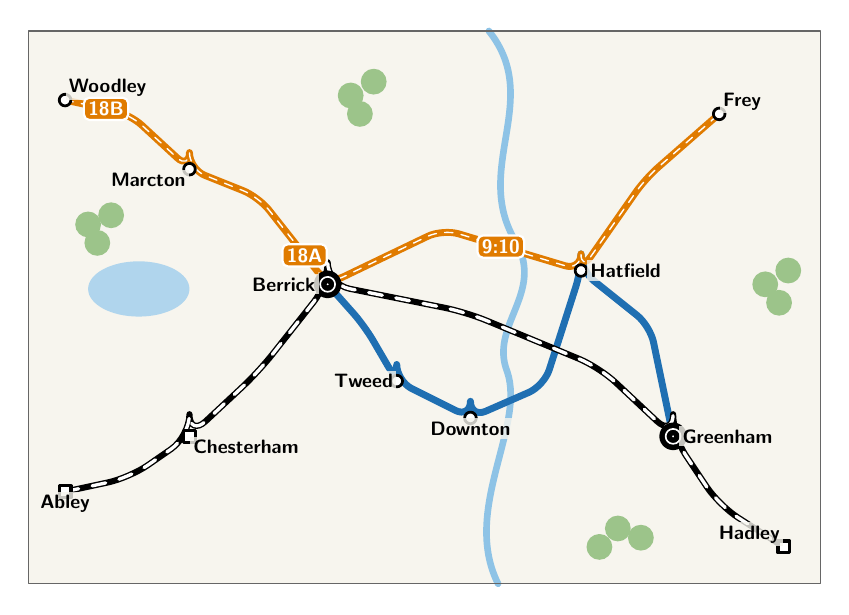
\begin{tikzpicture}[scale=0.585, line cap=round, line join=round]
\fill[mapbg] (0,0) rectangle (17.2,12);
\draw[river, line width=2.4pt] (10.0,12) .. controls (11.2,10.5) and (9.6,9.0) .. (10.6,7.4) .. controls (11.2,6.3) and (10.0,5.6) .. (10.4,4.6) .. controls (10.8,3.4) and (9.4,1.6) .. (10.2,0);
\fill[lake] (2.4,6.4) ellipse (1.1 and 0.6);
\fill[tree] (1.3,7.8) circle (0.28);
\fill[tree] (1.8,8.0) circle (0.28);
\fill[tree] (1.5,7.4) circle (0.28);
\fill[tree] (12.8,1.2) circle (0.28);
\fill[tree] (13.3,1.0) circle (0.28);
\fill[tree] (12.4,0.8) circle (0.28);
\fill[tree] (16.0,6.5) circle (0.28);
\fill[tree] (16.5,6.8) circle (0.28);
\fill[tree] (16.3,6.1) circle (0.28);
\fill[tree] (7.0,10.6) circle (0.28);
\fill[tree] (7.5,10.9) circle (0.28);
\fill[tree] (7.2,10.2) circle (0.28);
\draw[a34, line width=2.5pt, rounded corners=6pt] (6.50,6.50) -- (7.30,5.60) -- (8.00,4.40) -- (8.00,4.40) -- (9.60,3.60) -- (9.60,3.60) -- (11.20,4.30) -- (12.00,6.80) -- (12.00,6.80) -- (13.50,5.60) -- (14.00,3.20);
\draw[c18, line width=2.5pt, rounded corners=6pt] (0.80,10.50) -- (2.20,10.20) -- (3.50,9.00) -- (3.50,9.00) -- (5.00,8.40) -- (6.50,6.50) -- (6.50,6.50) -- (9.00,7.70) -- (12.00,6.80) -- (12.00,6.80) -- (13.40,8.80) -- (15.00,10.20);
\draw[white, line width=0.5pt, dash pattern=on 3pt off 3pt, rounded corners=6pt] (0.80,10.50) -- (2.20,10.20) -- (3.50,9.00) -- (3.50,9.00) -- (5.00,8.40) -- (6.50,6.50) -- (6.50,6.50) -- (9.00,7.70) -- (12.00,6.80) -- (12.00,6.80) -- (13.40,8.80) -- (15.00,10.20);
\draw[black, line width=2.2pt, rounded corners=8pt] (0.80,2.00) -- (2.20,2.30) -- (3.50,3.20) -- (3.50,3.20) -- (5.00,4.60) -- (6.50,6.50) -- (6.50,6.50) -- (9.50,5.90) -- (12.40,4.70) -- (14.00,3.20) -- (14.00,3.20) -- (15.00,1.70) -- (16.40,0.80);
\draw[white, line width=1.2pt, dash pattern=on 5pt off 5pt, rounded corners=8pt] (0.80,2.00) -- (2.20,2.30) -- (3.50,3.20) -- (3.50,3.20) -- (5.00,4.60) -- (6.50,6.50) -- (6.50,6.50) -- (9.50,5.90) -- (12.40,4.70) -- (14.00,3.20) -- (14.00,3.20) -- (15.00,1.70) -- (16.40,0.80);
\node[busstop, minimum size=4.2pt] at (0.8,10.5) {};
\node[above right, font=\scriptsize\bfseries, fill=mapbg, fill opacity=0.8, text opacity=1, inner sep=1.2pt] at (0.8,10.5) {Woodley};
\node[busstop, minimum size=4.2pt] at (3.5,9.0) {};
\node[below left, font=\scriptsize\bfseries, fill=mapbg, fill opacity=0.8, text opacity=1, inner sep=1.2pt] at (3.5,9.0) {Marcton};
\node[inter, minimum size=5.4pt] at (6.5,6.5) {};
\node[left=3pt, font=\scriptsize\bfseries, fill=mapbg, fill opacity=0.8, text opacity=1, inner sep=1.2pt] at (6.5,6.5) {Berrick};
\node[busstop, minimum size=4.2pt] at (8.0,4.4) {};
\node[left, font=\scriptsize\bfseries, fill=mapbg, fill opacity=0.8, text opacity=1, inner sep=1.2pt] at (8.0,4.4) {Tweed};
\node[busstop, minimum size=4.2pt] at (9.6,3.6) {};
\node[below, font=\scriptsize\bfseries, fill=mapbg, fill opacity=0.8, text opacity=1, inner sep=1.2pt] at (9.6,3.6) {Downton};
\node[busstop, minimum size=4.2pt] at (12.0,6.8) {};
\node[right=2pt, font=\scriptsize\bfseries, fill=mapbg, fill opacity=0.8, text opacity=1, inner sep=1.2pt] at (12.0,6.8) {Hatfield};
\node[inter, minimum size=5.4pt] at (14.0,3.2) {};
\node[right=2pt, font=\scriptsize\bfseries, fill=mapbg, fill opacity=0.8, text opacity=1, inner sep=1.2pt] at (14.0,3.2) {Greenham};
\node[busstop, minimum size=4.2pt] at (15.0,10.2) {};
\node[above right, font=\scriptsize\bfseries, fill=mapbg, fill opacity=0.8, text opacity=1, inner sep=1.2pt] at (15.0,10.2) {Frey};
\node[station, minimum size=4.2pt] at (0.8,2.0) {};
\node[below, font=\scriptsize\bfseries, fill=mapbg, fill opacity=0.8, text opacity=1, inner sep=1.2pt] at (0.8,2.0) {Abley};
\node[station, minimum size=4.2pt] at (3.5,3.2) {};
\node[below right, font=\scriptsize\bfseries, fill=mapbg, fill opacity=0.8, text opacity=1, inner sep=1.2pt] at (3.5,3.2) {Chesterham};
\node[station, minimum size=4.2pt] at (16.4,0.8) {};
\node[above left, font=\scriptsize\bfseries, fill=mapbg, fill opacity=0.8, text opacity=1, inner sep=1.2pt] at (16.4,0.8) {Hadley};
\node[busC] at (10.26,7.32) {9:10};
\node[busC] at (6.00,7.13) {18A};
\node[busC] at (1.69,10.31) {18B};
\draw[black!60] (0,0) rectangle (17.2,12);
\end{tikzpicture}\end{minipage}\hfill\begin{minipage}[t]{0.425\linewidth}\vspace{0pt}{\large\bfseries 2.}\ \ 
\begin{tikzpicture}[baseline=-3pt]\draw[thick, fill=white] (0,0) circle (0.5);\draw[thick] (0.000,0.360) -- (0.000,0.500);\draw[] (0.215,0.372) -- (0.250,0.433);\draw[] (0.372,0.215) -- (0.433,0.250);\draw[thick] (0.360,0.000) -- (0.500,0.000);\draw[] (0.372,-0.215) -- (0.433,-0.250);\draw[] (0.215,-0.372) -- (0.250,-0.433);\draw[thick] (0.000,-0.360) -- (0.000,-0.500);\draw[] (-0.215,-0.372) -- (-0.250,-0.433);\draw[] (-0.372,-0.215) -- (-0.433,-0.250);\draw[thick] (-0.360,-0.000) -- (-0.500,-0.000);\draw[] (-0.372,0.215) -- (-0.433,0.250);\draw[] (-0.215,0.372) -- (-0.250,0.433);\draw[line width=1.4pt] (0,0) -- (-0.238,0.138);\draw[line width=0.8pt] (0,0) -- (0.000,0.425);\fill (0,0) circle (1.2pt);\end{tikzpicture}\ \ {\bfseries Frozen at 10:00 --- C-18 buses only}\par\smallskip{\small\begin{tabularx}{\linewidth}{>{\raggedright\arraybackslash}p{3.15cm}|X|X}\textbf{Vehicle} & \textbf{Last stop} & \textbf{Next stop}\\ \hline
C-18 (09:10 from Woodley) & \ans{Berrick} & \ans{Hatfield}\\[-2pt] \multicolumn{3}{r}{\scriptsize\ans{18 of 26 min}}\\ \hline
C-18A (09:32 from Woodley) & \ans{Marcton} & \ans{Hatfield}\\[-2pt] \multicolumn{3}{r}{\scriptsize\ans{16 of 46 min; on the map between Marcton \& Berrick}}\\ \hline
C-18B (09:56 from Woodley) & \ans{Woodley} & \ans{Marcton}\\[-2pt] \multicolumn{3}{r}{\scriptsize\ans{4 of 14 min}}\\ \hline
C-18 (10:34 from Woodley) & \ans{---} & \ans{---}\\[-2pt] \multicolumn{3}{r}{\scriptsize\ans{Not left yet (leaves Woodley 10:34)}}\\ \hline\end{tabularx}}\end{minipage}\par\vspace{9pt}
\noindent\begin{minipage}[t]{0.555\linewidth}\vspace{0pt}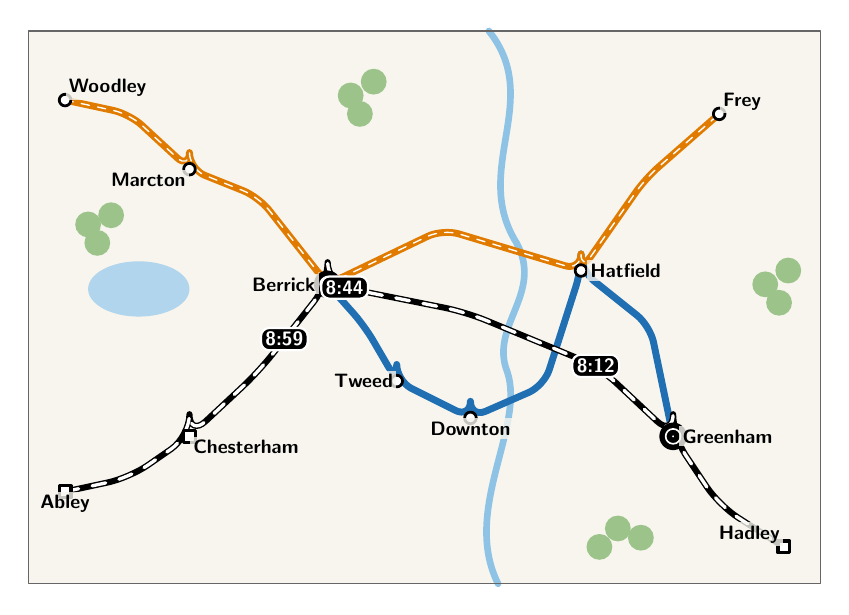
\begin{tikzpicture}[scale=0.585, line cap=round, line join=round]
\fill[mapbg] (0,0) rectangle (17.2,12);
\draw[river, line width=2.4pt] (10.0,12) .. controls (11.2,10.5) and (9.6,9.0) .. (10.6,7.4) .. controls (11.2,6.3) and (10.0,5.6) .. (10.4,4.6) .. controls (10.8,3.4) and (9.4,1.6) .. (10.2,0);
\fill[lake] (2.4,6.4) ellipse (1.1 and 0.6);
\fill[tree] (1.3,7.8) circle (0.28);
\fill[tree] (1.8,8.0) circle (0.28);
\fill[tree] (1.5,7.4) circle (0.28);
\fill[tree] (12.8,1.2) circle (0.28);
\fill[tree] (13.3,1.0) circle (0.28);
\fill[tree] (12.4,0.8) circle (0.28);
\fill[tree] (16.0,6.5) circle (0.28);
\fill[tree] (16.5,6.8) circle (0.28);
\fill[tree] (16.3,6.1) circle (0.28);
\fill[tree] (7.0,10.6) circle (0.28);
\fill[tree] (7.5,10.9) circle (0.28);
\fill[tree] (7.2,10.2) circle (0.28);
\draw[a34, line width=2.5pt, rounded corners=6pt] (6.50,6.50) -- (7.30,5.60) -- (8.00,4.40) -- (8.00,4.40) -- (9.60,3.60) -- (9.60,3.60) -- (11.20,4.30) -- (12.00,6.80) -- (12.00,6.80) -- (13.50,5.60) -- (14.00,3.20);
\draw[c18, line width=2.5pt, rounded corners=6pt] (0.80,10.50) -- (2.20,10.20) -- (3.50,9.00) -- (3.50,9.00) -- (5.00,8.40) -- (6.50,6.50) -- (6.50,6.50) -- (9.00,7.70) -- (12.00,6.80) -- (12.00,6.80) -- (13.40,8.80) -- (15.00,10.20);
\draw[white, line width=0.5pt, dash pattern=on 3pt off 3pt, rounded corners=6pt] (0.80,10.50) -- (2.20,10.20) -- (3.50,9.00) -- (3.50,9.00) -- (5.00,8.40) -- (6.50,6.50) -- (6.50,6.50) -- (9.00,7.70) -- (12.00,6.80) -- (12.00,6.80) -- (13.40,8.80) -- (15.00,10.20);
\draw[black, line width=2.2pt, rounded corners=8pt] (0.80,2.00) -- (2.20,2.30) -- (3.50,3.20) -- (3.50,3.20) -- (5.00,4.60) -- (6.50,6.50) -- (6.50,6.50) -- (9.50,5.90) -- (12.40,4.70) -- (14.00,3.20) -- (14.00,3.20) -- (15.00,1.70) -- (16.40,0.80);
\draw[white, line width=1.2pt, dash pattern=on 5pt off 5pt, rounded corners=8pt] (0.80,2.00) -- (2.20,2.30) -- (3.50,3.20) -- (3.50,3.20) -- (5.00,4.60) -- (6.50,6.50) -- (6.50,6.50) -- (9.50,5.90) -- (12.40,4.70) -- (14.00,3.20) -- (14.00,3.20) -- (15.00,1.70) -- (16.40,0.80);
\node[busstop, minimum size=4.2pt] at (0.8,10.5) {};
\node[above right, font=\scriptsize\bfseries, fill=mapbg, fill opacity=0.8, text opacity=1, inner sep=1.2pt] at (0.8,10.5) {Woodley};
\node[busstop, minimum size=4.2pt] at (3.5,9.0) {};
\node[below left, font=\scriptsize\bfseries, fill=mapbg, fill opacity=0.8, text opacity=1, inner sep=1.2pt] at (3.5,9.0) {Marcton};
\node[inter, minimum size=5.4pt] at (6.5,6.5) {};
\node[left=3pt, font=\scriptsize\bfseries, fill=mapbg, fill opacity=0.8, text opacity=1, inner sep=1.2pt] at (6.5,6.5) {Berrick};
\node[busstop, minimum size=4.2pt] at (8.0,4.4) {};
\node[left, font=\scriptsize\bfseries, fill=mapbg, fill opacity=0.8, text opacity=1, inner sep=1.2pt] at (8.0,4.4) {Tweed};
\node[busstop, minimum size=4.2pt] at (9.6,3.6) {};
\node[below, font=\scriptsize\bfseries, fill=mapbg, fill opacity=0.8, text opacity=1, inner sep=1.2pt] at (9.6,3.6) {Downton};
\node[busstop, minimum size=4.2pt] at (12.0,6.8) {};
\node[right=2pt, font=\scriptsize\bfseries, fill=mapbg, fill opacity=0.8, text opacity=1, inner sep=1.2pt] at (12.0,6.8) {Hatfield};
\node[inter, minimum size=5.4pt] at (14.0,3.2) {};
\node[right=2pt, font=\scriptsize\bfseries, fill=mapbg, fill opacity=0.8, text opacity=1, inner sep=1.2pt] at (14.0,3.2) {Greenham};
\node[busstop, minimum size=4.2pt] at (15.0,10.2) {};
\node[above right, font=\scriptsize\bfseries, fill=mapbg, fill opacity=0.8, text opacity=1, inner sep=1.2pt] at (15.0,10.2) {Frey};
\node[station, minimum size=4.2pt] at (0.8,2.0) {};
\node[below, font=\scriptsize\bfseries, fill=mapbg, fill opacity=0.8, text opacity=1, inner sep=1.2pt] at (0.8,2.0) {Abley};
\node[station, minimum size=4.2pt] at (3.5,3.2) {};
\node[below right, font=\scriptsize\bfseries, fill=mapbg, fill opacity=0.8, text opacity=1, inner sep=1.2pt] at (3.5,3.2) {Chesterham};
\node[station, minimum size=4.2pt] at (16.4,0.8) {};
\node[above left, font=\scriptsize\bfseries, fill=mapbg, fill opacity=0.8, text opacity=1, inner sep=1.2pt] at (16.4,0.8) {Hadley};
\node[train] at (12.32,4.73) {8:12};
\node[train] at (6.87,6.43) {8:44};
\node[train] at (5.56,5.31) {8:59};
\draw[black!60] (0,0) rectangle (17.2,12);
\end{tikzpicture}\end{minipage}\hfill\begin{minipage}[t]{0.425\linewidth}\vspace{0pt}{\large\bfseries 3.}\ \ 
\begin{tikzpicture}[baseline=-3pt]\draw[thick, fill=white] (0,0) circle (0.5);\draw[thick] (0.000,0.360) -- (0.000,0.500);\draw[] (0.215,0.372) -- (0.250,0.433);\draw[] (0.372,0.215) -- (0.433,0.250);\draw[thick] (0.360,0.000) -- (0.500,0.000);\draw[] (0.372,-0.215) -- (0.433,-0.250);\draw[] (0.215,-0.372) -- (0.250,-0.433);\draw[thick] (0.000,-0.360) -- (0.000,-0.500);\draw[] (-0.215,-0.372) -- (-0.250,-0.433);\draw[] (-0.372,-0.215) -- (-0.433,-0.250);\draw[thick] (-0.360,-0.000) -- (-0.500,-0.000);\draw[] (-0.372,0.215) -- (-0.433,0.250);\draw[] (-0.215,0.372) -- (-0.250,0.433);\draw[line width=1.4pt] (0,0) -- (-0.271,0.048);\draw[line width=0.8pt] (0,0) -- (0.368,-0.212);\fill (0,0) circle (1.2pt);\end{tikzpicture}\ \ {\bfseries Frozen at 09:20 --- trains only}\par\smallskip{\small\begin{tabularx}{\linewidth}{>{\raggedright\arraybackslash}p{3.15cm}|X|X}\textbf{Vehicle} & \textbf{Last stop} & \textbf{Next stop}\\ \hline
Train (08:12 from Abley) & \ans{Chesterham} & \ans{Greenham}\\[-2pt] \multicolumn{3}{r}{\scriptsize\ans{56 of 68 min; on the map between Berrick \& Greenham}}\\ \hline
Train (08:44 from Abley) & \ans{Berrick} & \ans{Hadley}\\[-2pt] \multicolumn{3}{r}{\scriptsize\ans{2 of 72 min; on the map between Berrick \& Greenham}}\\ \hline
Train (08:59 from Abley) & \ans{Abley} & \ans{Hadley}\\[-2pt] \multicolumn{3}{r}{\scriptsize\ans{21 of 80 min; on the map between Chesterham \& Berrick}}\\ \hline
Train (09:24 from Abley) & \ans{---} & \ans{---}\\[-2pt] \multicolumn{3}{r}{\scriptsize\ans{Not left yet (leaves Abley 09:24)}}\\ \hline
Train (09:55 from Abley) & \ans{---} & \ans{---}\\[-2pt] \multicolumn{3}{r}{\scriptsize\ans{Not left yet (leaves Abley 09:55)}}\\ \hline\end{tabularx}}\end{minipage}\par\vspace{9pt}
\clearpage
\noindent\begin{minipage}[t]{0.555\linewidth}\vspace{0pt}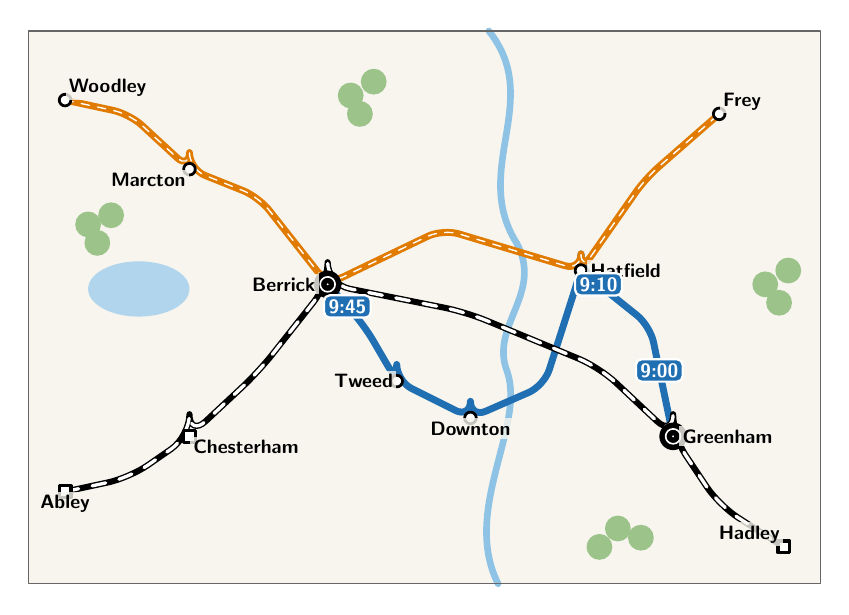
\begin{tikzpicture}[scale=0.585, line cap=round, line join=round]
\fill[mapbg] (0,0) rectangle (17.2,12);
\draw[river, line width=2.4pt] (10.0,12) .. controls (11.2,10.5) and (9.6,9.0) .. (10.6,7.4) .. controls (11.2,6.3) and (10.0,5.6) .. (10.4,4.6) .. controls (10.8,3.4) and (9.4,1.6) .. (10.2,0);
\fill[lake] (2.4,6.4) ellipse (1.1 and 0.6);
\fill[tree] (1.3,7.8) circle (0.28);
\fill[tree] (1.8,8.0) circle (0.28);
\fill[tree] (1.5,7.4) circle (0.28);
\fill[tree] (12.8,1.2) circle (0.28);
\fill[tree] (13.3,1.0) circle (0.28);
\fill[tree] (12.4,0.8) circle (0.28);
\fill[tree] (16.0,6.5) circle (0.28);
\fill[tree] (16.5,6.8) circle (0.28);
\fill[tree] (16.3,6.1) circle (0.28);
\fill[tree] (7.0,10.6) circle (0.28);
\fill[tree] (7.5,10.9) circle (0.28);
\fill[tree] (7.2,10.2) circle (0.28);
\draw[a34, line width=2.5pt, rounded corners=6pt] (6.50,6.50) -- (7.30,5.60) -- (8.00,4.40) -- (8.00,4.40) -- (9.60,3.60) -- (9.60,3.60) -- (11.20,4.30) -- (12.00,6.80) -- (12.00,6.80) -- (13.50,5.60) -- (14.00,3.20);
\draw[c18, line width=2.5pt, rounded corners=6pt] (0.80,10.50) -- (2.20,10.20) -- (3.50,9.00) -- (3.50,9.00) -- (5.00,8.40) -- (6.50,6.50) -- (6.50,6.50) -- (9.00,7.70) -- (12.00,6.80) -- (12.00,6.80) -- (13.40,8.80) -- (15.00,10.20);
\draw[white, line width=0.5pt, dash pattern=on 3pt off 3pt, rounded corners=6pt] (0.80,10.50) -- (2.20,10.20) -- (3.50,9.00) -- (3.50,9.00) -- (5.00,8.40) -- (6.50,6.50) -- (6.50,6.50) -- (9.00,7.70) -- (12.00,6.80) -- (12.00,6.80) -- (13.40,8.80) -- (15.00,10.20);
\draw[black, line width=2.2pt, rounded corners=8pt] (0.80,2.00) -- (2.20,2.30) -- (3.50,3.20) -- (3.50,3.20) -- (5.00,4.60) -- (6.50,6.50) -- (6.50,6.50) -- (9.50,5.90) -- (12.40,4.70) -- (14.00,3.20) -- (14.00,3.20) -- (15.00,1.70) -- (16.40,0.80);
\draw[white, line width=1.2pt, dash pattern=on 5pt off 5pt, rounded corners=8pt] (0.80,2.00) -- (2.20,2.30) -- (3.50,3.20) -- (3.50,3.20) -- (5.00,4.60) -- (6.50,6.50) -- (6.50,6.50) -- (9.50,5.90) -- (12.40,4.70) -- (14.00,3.20) -- (14.00,3.20) -- (15.00,1.70) -- (16.40,0.80);
\node[busstop, minimum size=4.2pt] at (0.8,10.5) {};
\node[above right, font=\scriptsize\bfseries, fill=mapbg, fill opacity=0.8, text opacity=1, inner sep=1.2pt] at (0.8,10.5) {Woodley};
\node[busstop, minimum size=4.2pt] at (3.5,9.0) {};
\node[below left, font=\scriptsize\bfseries, fill=mapbg, fill opacity=0.8, text opacity=1, inner sep=1.2pt] at (3.5,9.0) {Marcton};
\node[inter, minimum size=5.4pt] at (6.5,6.5) {};
\node[left=3pt, font=\scriptsize\bfseries, fill=mapbg, fill opacity=0.8, text opacity=1, inner sep=1.2pt] at (6.5,6.5) {Berrick};
\node[busstop, minimum size=4.2pt] at (8.0,4.4) {};
\node[left, font=\scriptsize\bfseries, fill=mapbg, fill opacity=0.8, text opacity=1, inner sep=1.2pt] at (8.0,4.4) {Tweed};
\node[busstop, minimum size=4.2pt] at (9.6,3.6) {};
\node[below, font=\scriptsize\bfseries, fill=mapbg, fill opacity=0.8, text opacity=1, inner sep=1.2pt] at (9.6,3.6) {Downton};
\node[busstop, minimum size=4.2pt] at (12.0,6.8) {};
\node[right=2pt, font=\scriptsize\bfseries, fill=mapbg, fill opacity=0.8, text opacity=1, inner sep=1.2pt] at (12.0,6.8) {Hatfield};
\node[inter, minimum size=5.4pt] at (14.0,3.2) {};
\node[right=2pt, font=\scriptsize\bfseries, fill=mapbg, fill opacity=0.8, text opacity=1, inner sep=1.2pt] at (14.0,3.2) {Greenham};
\node[busstop, minimum size=4.2pt] at (15.0,10.2) {};
\node[above right, font=\scriptsize\bfseries, fill=mapbg, fill opacity=0.8, text opacity=1, inner sep=1.2pt] at (15.0,10.2) {Frey};
\node[station, minimum size=4.2pt] at (0.8,2.0) {};
\node[below, font=\scriptsize\bfseries, fill=mapbg, fill opacity=0.8, text opacity=1, inner sep=1.2pt] at (0.8,2.0) {Abley};
\node[station, minimum size=4.2pt] at (3.5,3.2) {};
\node[below right, font=\scriptsize\bfseries, fill=mapbg, fill opacity=0.8, text opacity=1, inner sep=1.2pt] at (3.5,3.2) {Chesterham};
\node[station, minimum size=4.2pt] at (16.4,0.8) {};
\node[above left, font=\scriptsize\bfseries, fill=mapbg, fill opacity=0.8, text opacity=1, inner sep=1.2pt] at (16.4,0.8) {Hadley};
\node[busA] at (13.70,4.63) {9:00};
\node[busA] at (12.38,6.50) {9:10};
\node[busA] at (6.93,6.02) {9:45};
\draw[black!60] (0,0) rectangle (17.2,12);
\end{tikzpicture}\end{minipage}\hfill\begin{minipage}[t]{0.425\linewidth}\vspace{0pt}{\large\bfseries 4.}\ \ 
\begin{tikzpicture}[baseline=-3pt]\draw[thick, fill=white] (0,0) circle (0.5);\draw[thick] (0.000,0.360) -- (0.000,0.500);\draw[] (0.215,0.372) -- (0.250,0.433);\draw[] (0.372,0.215) -- (0.433,0.250);\draw[thick] (0.360,0.000) -- (0.500,0.000);\draw[] (0.372,-0.215) -- (0.433,-0.250);\draw[] (0.215,-0.372) -- (0.250,-0.433);\draw[thick] (0.000,-0.360) -- (0.000,-0.500);\draw[] (-0.215,-0.372) -- (-0.250,-0.433);\draw[] (-0.372,-0.215) -- (-0.433,-0.250);\draw[thick] (-0.360,-0.000) -- (-0.500,-0.000);\draw[] (-0.372,0.215) -- (-0.433,0.250);\draw[] (-0.215,0.372) -- (-0.250,0.433);\draw[line width=1.4pt] (0,0) -- (-0.249,0.116);\draw[line width=0.8pt] (0,0) -- (-0.368,0.213);\fill (0,0) circle (1.2pt);\end{tikzpicture}\ \ {\bfseries Frozen at 09:50 --- A34 buses only}\par\smallskip{\small\begin{tabularx}{\linewidth}{>{\raggedright\arraybackslash}p{3.15cm}|X|X}\textbf{Vehicle} & \textbf{Last stop} & \textbf{Next stop}\\ \hline
A34 (09:00 from Berrick) & \ans{Hatfield} & \ans{Greenham}\\[-2pt] \multicolumn{3}{r}{\scriptsize\ans{12 of 18 min}}\\ \hline
A34 (09:10 from Berrick) & \ans{Hatfield} & \ans{Greenham}\\[-2pt] \multicolumn{3}{r}{\scriptsize\ans{2 of 18 min}}\\ \hline
A34 (09:45 from Berrick) & \ans{Berrick} & \ans{Tweed}\\[-2pt] \multicolumn{3}{r}{\scriptsize\ans{5 of 20 min}}\\ \hline\end{tabularx}}\end{minipage}\par\vspace{9pt}
\noindent\begin{minipage}[t]{0.555\linewidth}\vspace{0pt}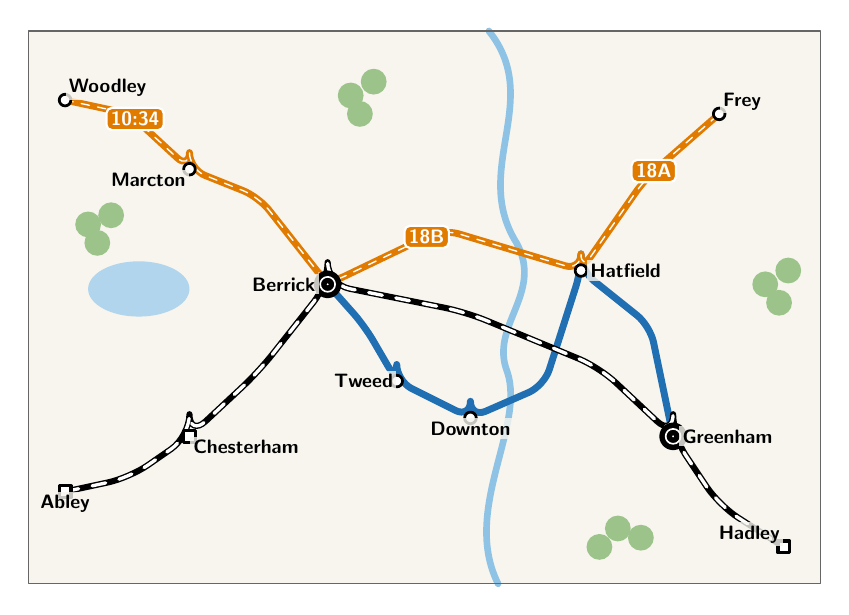
\begin{tikzpicture}[scale=0.585, line cap=round, line join=round]
\fill[mapbg] (0,0) rectangle (17.2,12);
\draw[river, line width=2.4pt] (10.0,12) .. controls (11.2,10.5) and (9.6,9.0) .. (10.6,7.4) .. controls (11.2,6.3) and (10.0,5.6) .. (10.4,4.6) .. controls (10.8,3.4) and (9.4,1.6) .. (10.2,0);
\fill[lake] (2.4,6.4) ellipse (1.1 and 0.6);
\fill[tree] (1.3,7.8) circle (0.28);
\fill[tree] (1.8,8.0) circle (0.28);
\fill[tree] (1.5,7.4) circle (0.28);
\fill[tree] (12.8,1.2) circle (0.28);
\fill[tree] (13.3,1.0) circle (0.28);
\fill[tree] (12.4,0.8) circle (0.28);
\fill[tree] (16.0,6.5) circle (0.28);
\fill[tree] (16.5,6.8) circle (0.28);
\fill[tree] (16.3,6.1) circle (0.28);
\fill[tree] (7.0,10.6) circle (0.28);
\fill[tree] (7.5,10.9) circle (0.28);
\fill[tree] (7.2,10.2) circle (0.28);
\draw[a34, line width=2.5pt, rounded corners=6pt] (6.50,6.50) -- (7.30,5.60) -- (8.00,4.40) -- (8.00,4.40) -- (9.60,3.60) -- (9.60,3.60) -- (11.20,4.30) -- (12.00,6.80) -- (12.00,6.80) -- (13.50,5.60) -- (14.00,3.20);
\draw[c18, line width=2.5pt, rounded corners=6pt] (0.80,10.50) -- (2.20,10.20) -- (3.50,9.00) -- (3.50,9.00) -- (5.00,8.40) -- (6.50,6.50) -- (6.50,6.50) -- (9.00,7.70) -- (12.00,6.80) -- (12.00,6.80) -- (13.40,8.80) -- (15.00,10.20);
\draw[white, line width=0.5pt, dash pattern=on 3pt off 3pt, rounded corners=6pt] (0.80,10.50) -- (2.20,10.20) -- (3.50,9.00) -- (3.50,9.00) -- (5.00,8.40) -- (6.50,6.50) -- (6.50,6.50) -- (9.00,7.70) -- (12.00,6.80) -- (12.00,6.80) -- (13.40,8.80) -- (15.00,10.20);
\draw[black, line width=2.2pt, rounded corners=8pt] (0.80,2.00) -- (2.20,2.30) -- (3.50,3.20) -- (3.50,3.20) -- (5.00,4.60) -- (6.50,6.50) -- (6.50,6.50) -- (9.50,5.90) -- (12.40,4.70) -- (14.00,3.20) -- (14.00,3.20) -- (15.00,1.70) -- (16.40,0.80);
\draw[white, line width=1.2pt, dash pattern=on 5pt off 5pt, rounded corners=8pt] (0.80,2.00) -- (2.20,2.30) -- (3.50,3.20) -- (3.50,3.20) -- (5.00,4.60) -- (6.50,6.50) -- (6.50,6.50) -- (9.50,5.90) -- (12.40,4.70) -- (14.00,3.20) -- (14.00,3.20) -- (15.00,1.70) -- (16.40,0.80);
\node[busstop, minimum size=4.2pt] at (0.8,10.5) {};
\node[above right, font=\scriptsize\bfseries, fill=mapbg, fill opacity=0.8, text opacity=1, inner sep=1.2pt] at (0.8,10.5) {Woodley};
\node[busstop, minimum size=4.2pt] at (3.5,9.0) {};
\node[below left, font=\scriptsize\bfseries, fill=mapbg, fill opacity=0.8, text opacity=1, inner sep=1.2pt] at (3.5,9.0) {Marcton};
\node[inter, minimum size=5.4pt] at (6.5,6.5) {};
\node[left=3pt, font=\scriptsize\bfseries, fill=mapbg, fill opacity=0.8, text opacity=1, inner sep=1.2pt] at (6.5,6.5) {Berrick};
\node[busstop, minimum size=4.2pt] at (8.0,4.4) {};
\node[left, font=\scriptsize\bfseries, fill=mapbg, fill opacity=0.8, text opacity=1, inner sep=1.2pt] at (8.0,4.4) {Tweed};
\node[busstop, minimum size=4.2pt] at (9.6,3.6) {};
\node[below, font=\scriptsize\bfseries, fill=mapbg, fill opacity=0.8, text opacity=1, inner sep=1.2pt] at (9.6,3.6) {Downton};
\node[busstop, minimum size=4.2pt] at (12.0,6.8) {};
\node[right=2pt, font=\scriptsize\bfseries, fill=mapbg, fill opacity=0.8, text opacity=1, inner sep=1.2pt] at (12.0,6.8) {Hatfield};
\node[inter, minimum size=5.4pt] at (14.0,3.2) {};
\node[right=2pt, font=\scriptsize\bfseries, fill=mapbg, fill opacity=0.8, text opacity=1, inner sep=1.2pt] at (14.0,3.2) {Greenham};
\node[busstop, minimum size=4.2pt] at (15.0,10.2) {};
\node[above right, font=\scriptsize\bfseries, fill=mapbg, fill opacity=0.8, text opacity=1, inner sep=1.2pt] at (15.0,10.2) {Frey};
\node[station, minimum size=4.2pt] at (0.8,2.0) {};
\node[below, font=\scriptsize\bfseries, fill=mapbg, fill opacity=0.8, text opacity=1, inner sep=1.2pt] at (0.8,2.0) {Abley};
\node[station, minimum size=4.2pt] at (3.5,3.2) {};
\node[below right, font=\scriptsize\bfseries, fill=mapbg, fill opacity=0.8, text opacity=1, inner sep=1.2pt] at (3.5,3.2) {Chesterham};
\node[station, minimum size=4.2pt] at (16.4,0.8) {};
\node[above left, font=\scriptsize\bfseries, fill=mapbg, fill opacity=0.8, text opacity=1, inner sep=1.2pt] at (16.4,0.8) {Hadley};
\node[busC] at (13.58,8.96) {18A};
\node[busC] at (8.65,7.53) {18B};
\node[busC] at (2.32,10.09) {10:34};
\draw[black!60] (0,0) rectangle (17.2,12);
\end{tikzpicture}\end{minipage}\hfill\begin{minipage}[t]{0.425\linewidth}\vspace{0pt}{\large\bfseries 5.}\ \ 
\begin{tikzpicture}[baseline=-3pt]\draw[thick, fill=white] (0,0) circle (0.5);\draw[thick] (0.000,0.360) -- (0.000,0.500);\draw[] (0.215,0.372) -- (0.250,0.433);\draw[] (0.372,0.215) -- (0.433,0.250);\draw[thick] (0.360,0.000) -- (0.500,0.000);\draw[] (0.372,-0.215) -- (0.433,-0.250);\draw[] (0.215,-0.372) -- (0.250,-0.433);\draw[thick] (0.000,-0.360) -- (0.000,-0.500);\draw[] (-0.215,-0.372) -- (-0.250,-0.433);\draw[] (-0.372,-0.215) -- (-0.433,-0.250);\draw[thick] (-0.360,-0.000) -- (-0.500,-0.000);\draw[] (-0.372,0.215) -- (-0.433,0.250);\draw[] (-0.215,0.372) -- (-0.250,0.433);\draw[line width=1.4pt] (0,0) -- (-0.177,0.211);\draw[line width=0.8pt] (0,0) -- (-0.368,-0.212);\fill (0,0) circle (1.2pt);\end{tikzpicture}\ \ {\bfseries Frozen at 10:40 --- C-18 buses only}\par\smallskip{\small\begin{tabularx}{\linewidth}{>{\raggedright\arraybackslash}p{3.15cm}|X|X}\textbf{Vehicle} & \textbf{Last stop} & \textbf{Next stop}\\ \hline
C-18 (09:10 from Woodley) & \ans{---} & \ans{---}\\[-2pt] \multicolumn{3}{r}{\scriptsize\ans{Finished (reached Frey 10:25)}}\\ \hline
C-18A (09:32 from Woodley) & \ans{Hatfield} & \ans{Frey}\\[-2pt] \multicolumn{3}{r}{\scriptsize\ans{10 of 17 min}}\\ \hline
C-18B (09:56 from Woodley) & \ans{Marcton} & \ans{Frey}\\[-2pt] \multicolumn{3}{r}{\scriptsize\ans{30 of 62 min; on the map between Berrick \& Hatfield}}\\ \hline
C-18 (10:34 from Woodley) & \ans{Woodley} & \ans{Marcton}\\[-2pt] \multicolumn{3}{r}{\scriptsize\ans{6 of 12 min}}\\ \hline\end{tabularx}}\end{minipage}\par\vspace{9pt}
\noindent\begin{minipage}[t]{0.555\linewidth}\vspace{0pt}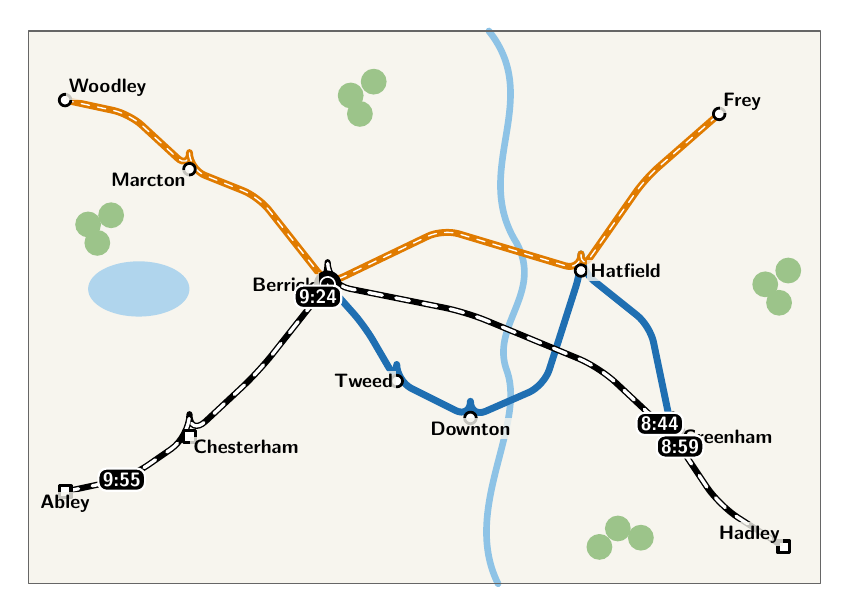
\begin{tikzpicture}[scale=0.585, line cap=round, line join=round]
\fill[mapbg] (0,0) rectangle (17.2,12);
\draw[river, line width=2.4pt] (10.0,12) .. controls (11.2,10.5) and (9.6,9.0) .. (10.6,7.4) .. controls (11.2,6.3) and (10.0,5.6) .. (10.4,4.6) .. controls (10.8,3.4) and (9.4,1.6) .. (10.2,0);
\fill[lake] (2.4,6.4) ellipse (1.1 and 0.6);
\fill[tree] (1.3,7.8) circle (0.28);
\fill[tree] (1.8,8.0) circle (0.28);
\fill[tree] (1.5,7.4) circle (0.28);
\fill[tree] (12.8,1.2) circle (0.28);
\fill[tree] (13.3,1.0) circle (0.28);
\fill[tree] (12.4,0.8) circle (0.28);
\fill[tree] (16.0,6.5) circle (0.28);
\fill[tree] (16.5,6.8) circle (0.28);
\fill[tree] (16.3,6.1) circle (0.28);
\fill[tree] (7.0,10.6) circle (0.28);
\fill[tree] (7.5,10.9) circle (0.28);
\fill[tree] (7.2,10.2) circle (0.28);
\draw[a34, line width=2.5pt, rounded corners=6pt] (6.50,6.50) -- (7.30,5.60) -- (8.00,4.40) -- (8.00,4.40) -- (9.60,3.60) -- (9.60,3.60) -- (11.20,4.30) -- (12.00,6.80) -- (12.00,6.80) -- (13.50,5.60) -- (14.00,3.20);
\draw[c18, line width=2.5pt, rounded corners=6pt] (0.80,10.50) -- (2.20,10.20) -- (3.50,9.00) -- (3.50,9.00) -- (5.00,8.40) -- (6.50,6.50) -- (6.50,6.50) -- (9.00,7.70) -- (12.00,6.80) -- (12.00,6.80) -- (13.40,8.80) -- (15.00,10.20);
\draw[white, line width=0.5pt, dash pattern=on 3pt off 3pt, rounded corners=6pt] (0.80,10.50) -- (2.20,10.20) -- (3.50,9.00) -- (3.50,9.00) -- (5.00,8.40) -- (6.50,6.50) -- (6.50,6.50) -- (9.00,7.70) -- (12.00,6.80) -- (12.00,6.80) -- (13.40,8.80) -- (15.00,10.20);
\draw[black, line width=2.2pt, rounded corners=8pt] (0.80,2.00) -- (2.20,2.30) -- (3.50,3.20) -- (3.50,3.20) -- (5.00,4.60) -- (6.50,6.50) -- (6.50,6.50) -- (9.50,5.90) -- (12.40,4.70) -- (14.00,3.20) -- (14.00,3.20) -- (15.00,1.70) -- (16.40,0.80);
\draw[white, line width=1.2pt, dash pattern=on 5pt off 5pt, rounded corners=8pt] (0.80,2.00) -- (2.20,2.30) -- (3.50,3.20) -- (3.50,3.20) -- (5.00,4.60) -- (6.50,6.50) -- (6.50,6.50) -- (9.50,5.90) -- (12.40,4.70) -- (14.00,3.20) -- (14.00,3.20) -- (15.00,1.70) -- (16.40,0.80);
\node[busstop, minimum size=4.2pt] at (0.8,10.5) {};
\node[above right, font=\scriptsize\bfseries, fill=mapbg, fill opacity=0.8, text opacity=1, inner sep=1.2pt] at (0.8,10.5) {Woodley};
\node[busstop, minimum size=4.2pt] at (3.5,9.0) {};
\node[below left, font=\scriptsize\bfseries, fill=mapbg, fill opacity=0.8, text opacity=1, inner sep=1.2pt] at (3.5,9.0) {Marcton};
\node[inter, minimum size=5.4pt] at (6.5,6.5) {};
\node[left=3pt, font=\scriptsize\bfseries, fill=mapbg, fill opacity=0.8, text opacity=1, inner sep=1.2pt] at (6.5,6.5) {Berrick};
\node[busstop, minimum size=4.2pt] at (8.0,4.4) {};
\node[left, font=\scriptsize\bfseries, fill=mapbg, fill opacity=0.8, text opacity=1, inner sep=1.2pt] at (8.0,4.4) {Tweed};
\node[busstop, minimum size=4.2pt] at (9.6,3.6) {};
\node[below, font=\scriptsize\bfseries, fill=mapbg, fill opacity=0.8, text opacity=1, inner sep=1.2pt] at (9.6,3.6) {Downton};
\node[busstop, minimum size=4.2pt] at (12.0,6.8) {};
\node[right=2pt, font=\scriptsize\bfseries, fill=mapbg, fill opacity=0.8, text opacity=1, inner sep=1.2pt] at (12.0,6.8) {Hatfield};
\node[inter, minimum size=5.4pt] at (14.0,3.2) {};
\node[right=2pt, font=\scriptsize\bfseries, fill=mapbg, fill opacity=0.8, text opacity=1, inner sep=1.2pt] at (14.0,3.2) {Greenham};
\node[busstop, minimum size=4.2pt] at (15.0,10.2) {};
\node[above right, font=\scriptsize\bfseries, fill=mapbg, fill opacity=0.8, text opacity=1, inner sep=1.2pt] at (15.0,10.2) {Frey};
\node[station, minimum size=4.2pt] at (0.8,2.0) {};
\node[below, font=\scriptsize\bfseries, fill=mapbg, fill opacity=0.8, text opacity=1, inner sep=1.2pt] at (0.8,2.0) {Abley};
\node[station, minimum size=4.2pt] at (3.5,3.2) {};
\node[below right, font=\scriptsize\bfseries, fill=mapbg, fill opacity=0.8, text opacity=1, inner sep=1.2pt] at (3.5,3.2) {Chesterham};
\node[station, minimum size=4.2pt] at (16.4,0.8) {};
\node[above left, font=\scriptsize\bfseries, fill=mapbg, fill opacity=0.8, text opacity=1, inner sep=1.2pt] at (16.4,0.8) {Hadley};
\node[train] at (13.71,3.47) {8:44};
\node[train] at (14.15,2.98) {8:59};
\node[train] at (6.29,6.23) {9:24};
\node[train] at (2.03,2.26) {9:55};
\draw[black!60] (0,0) rectangle (17.2,12);
\end{tikzpicture}\end{minipage}\hfill\begin{minipage}[t]{0.425\linewidth}\vspace{0pt}{\large\bfseries 6.}\ \ 
\begin{tikzpicture}[baseline=-3pt]\draw[thick, fill=white] (0,0) circle (0.5);\draw[thick] (0.000,0.360) -- (0.000,0.500);\draw[] (0.215,0.372) -- (0.250,0.433);\draw[] (0.372,0.215) -- (0.433,0.250);\draw[thick] (0.360,0.000) -- (0.500,0.000);\draw[] (0.372,-0.215) -- (0.433,-0.250);\draw[] (0.215,-0.372) -- (0.250,-0.433);\draw[thick] (0.000,-0.360) -- (0.000,-0.500);\draw[] (-0.215,-0.372) -- (-0.250,-0.433);\draw[] (-0.372,-0.215) -- (-0.433,-0.250);\draw[thick] (-0.360,-0.000) -- (-0.500,-0.000);\draw[] (-0.372,0.215) -- (-0.433,0.250);\draw[] (-0.215,0.372) -- (-0.250,0.433);\draw[line width=1.4pt] (0,0) -- (-0.238,0.138);\draw[line width=0.8pt] (0,0) -- (0.000,0.425);\fill (0,0) circle (1.2pt);\end{tikzpicture}\ \ {\bfseries Frozen at 10:00 --- trains only}\par\smallskip{\small\begin{tabularx}{\linewidth}{>{\raggedright\arraybackslash}p{3.15cm}|X|X}\textbf{Vehicle} & \textbf{Last stop} & \textbf{Next stop}\\ \hline
Train (08:12 from Abley) & \ans{---} & \ans{---}\\[-2pt] \multicolumn{3}{r}{\scriptsize\ans{Finished (reached Hadley 09:58)}}\\ \hline
Train (08:44 from Abley) & \ans{Berrick} & \ans{Hadley}\\[-2pt] \multicolumn{3}{r}{\scriptsize\ans{42 of 72 min; on the map between Berrick \& Greenham}}\\ \hline
Train (08:59 from Abley) & \ans{Abley} & \ans{Hadley}\\[-2pt] \multicolumn{3}{r}{\scriptsize\ans{61 of 80 min; on the map between Greenham \& Hadley}}\\ \hline
Train (09:24 from Abley) & \ans{Chesterham} & \ans{Berrick}\\[-2pt] \multicolumn{3}{r}{\scriptsize\ans{12 of 13 min}}\\ \hline
Train (09:55 from Abley) & \ans{Abley} & \ans{Chesterham}\\[-2pt] \multicolumn{3}{r}{\scriptsize\ans{5 of 12 min}}\\ \hline\end{tabularx}}\end{minipage}\par\vspace{9pt}
\clearpage
{\large\bfseries 7.\ \ Challenge --- frozen at 10:20}\par\smallskip\begin{center}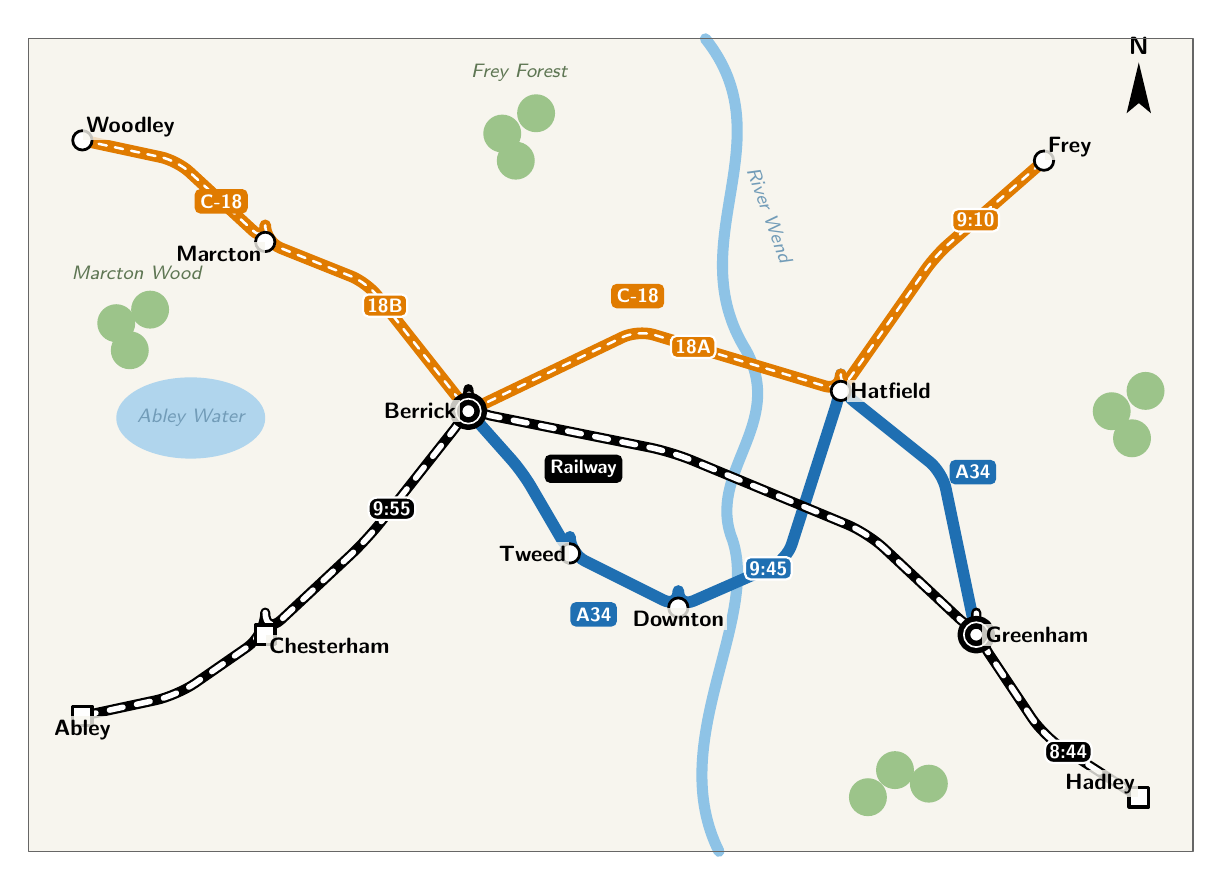
\begin{tikzpicture}[scale=0.86, line cap=round, line join=round]
\fill[mapbg] (0,0) rectangle (17.2,12);
\draw[river, line width=4.0pt] (10.0,12) .. controls (11.2,10.5) and (9.6,9.0) .. (10.6,7.4) .. controls (11.2,6.3) and (10.0,5.6) .. (10.4,4.6) .. controls (10.8,3.4) and (9.4,1.6) .. (10.2,0);
\fill[lake] (2.4,6.4) ellipse (1.1 and 0.6);
\node[font=\scriptsize\itshape, text=riverblue!80!black] at (2.4,6.4) {Abley Water};
\node[font=\scriptsize\itshape, text=riverblue!80!black, rotate=-70] at (10.95,9.4) {River Wend};
\fill[tree] (1.3,7.8) circle (0.28);
\fill[tree] (1.8,8.0) circle (0.28);
\fill[tree] (1.5,7.4) circle (0.28);
\fill[tree] (12.8,1.2) circle (0.28);
\fill[tree] (13.3,1.0) circle (0.28);
\fill[tree] (12.4,0.8) circle (0.28);
\fill[tree] (16.0,6.5) circle (0.28);
\fill[tree] (16.5,6.8) circle (0.28);
\fill[tree] (16.3,6.1) circle (0.28);
\fill[tree] (7.0,10.6) circle (0.28);
\fill[tree] (7.5,10.9) circle (0.28);
\fill[tree] (7.2,10.2) circle (0.28);
\node[font=\scriptsize\itshape, text=tree!60!black] at (1.6,8.55) {Marcton Wood};
\node[font=\scriptsize\itshape, text=tree!60!black] at (7.25,11.5) {Frey Forest};
\draw[a34, line width=4.2pt, rounded corners=6pt] (6.50,6.50) -- (7.30,5.60) -- (8.00,4.40) -- (8.00,4.40) -- (9.60,3.60) -- (9.60,3.60) -- (11.20,4.30) -- (12.00,6.80) -- (12.00,6.80) -- (13.50,5.60) -- (14.00,3.20);
\draw[c18, line width=4.2pt, rounded corners=6pt] (0.80,10.50) -- (2.20,10.20) -- (3.50,9.00) -- (3.50,9.00) -- (5.00,8.40) -- (6.50,6.50) -- (6.50,6.50) -- (9.00,7.70) -- (12.00,6.80) -- (12.00,6.80) -- (13.40,8.80) -- (15.00,10.20);
\draw[white, line width=0.9pt, dash pattern=on 3pt off 3pt, rounded corners=6pt] (0.80,10.50) -- (2.20,10.20) -- (3.50,9.00) -- (3.50,9.00) -- (5.00,8.40) -- (6.50,6.50) -- (6.50,6.50) -- (9.00,7.70) -- (12.00,6.80) -- (12.00,6.80) -- (13.40,8.80) -- (15.00,10.20);
\draw[black, line width=3.6pt, rounded corners=8pt] (0.80,2.00) -- (2.20,2.30) -- (3.50,3.20) -- (3.50,3.20) -- (5.00,4.60) -- (6.50,6.50) -- (6.50,6.50) -- (9.50,5.90) -- (12.40,4.70) -- (14.00,3.20) -- (14.00,3.20) -- (15.00,1.70) -- (16.40,0.80);
\draw[white, line width=2.0pt, dash pattern=on 5pt off 5pt, rounded corners=8pt] (0.80,2.00) -- (2.20,2.30) -- (3.50,3.20) -- (3.50,3.20) -- (5.00,4.60) -- (6.50,6.50) -- (6.50,6.50) -- (9.50,5.90) -- (12.40,4.70) -- (14.00,3.20) -- (14.00,3.20) -- (15.00,1.70) -- (16.40,0.80);
\node[badge=a34] at (8.35,3.5) {A34};
\node[badge=a34] at (13.95,5.6) {A34};
\node[badge=c18] at (9.0,8.2) {C-18};
\node[badge=c18] at (2.85,9.6) {C-18};
\node[badge=black] at (8.2,5.65) {Railway};
\begin{scope}[shift={(16.4,10.9)}]\fill[black] (0,0.75) -- (0.18,0) -- (0,0.15) -- (-0.18,0) -- cycle; \node[font=\bfseries\small] at (0,1.0) {N};\end{scope}
\node[busstop, minimum size=7.0pt] at (0.8,10.5) {};
\node[above right, font=\footnotesize\bfseries, fill=mapbg, fill opacity=0.8, text opacity=1, inner sep=1.2pt] at (0.8,10.5) {Woodley};
\node[busstop, minimum size=7.0pt] at (3.5,9.0) {};
\node[below left, font=\footnotesize\bfseries, fill=mapbg, fill opacity=0.8, text opacity=1, inner sep=1.2pt] at (3.5,9.0) {Marcton};
\node[inter, minimum size=9.0pt] at (6.5,6.5) {};
\node[left=3pt, font=\footnotesize\bfseries, fill=mapbg, fill opacity=0.8, text opacity=1, inner sep=1.2pt] at (6.5,6.5) {Berrick};
\node[busstop, minimum size=7.0pt] at (8.0,4.4) {};
\node[left, font=\footnotesize\bfseries, fill=mapbg, fill opacity=0.8, text opacity=1, inner sep=1.2pt] at (8.0,4.4) {Tweed};
\node[busstop, minimum size=7.0pt] at (9.6,3.6) {};
\node[below, font=\footnotesize\bfseries, fill=mapbg, fill opacity=0.8, text opacity=1, inner sep=1.2pt] at (9.6,3.6) {Downton};
\node[busstop, minimum size=7.0pt] at (12.0,6.8) {};
\node[right=2pt, font=\footnotesize\bfseries, fill=mapbg, fill opacity=0.8, text opacity=1, inner sep=1.2pt] at (12.0,6.8) {Hatfield};
\node[inter, minimum size=9.0pt] at (14.0,3.2) {};
\node[right=2pt, font=\footnotesize\bfseries, fill=mapbg, fill opacity=0.8, text opacity=1, inner sep=1.2pt] at (14.0,3.2) {Greenham};
\node[busstop, minimum size=7.0pt] at (15.0,10.2) {};
\node[above right, font=\footnotesize\bfseries, fill=mapbg, fill opacity=0.8, text opacity=1, inner sep=1.2pt] at (15.0,10.2) {Frey};
\node[station, minimum size=7.0pt] at (0.8,2.0) {};
\node[below, font=\footnotesize\bfseries, fill=mapbg, fill opacity=0.8, text opacity=1, inner sep=1.2pt] at (0.8,2.0) {Abley};
\node[station, minimum size=7.0pt] at (3.5,3.2) {};
\node[below right, font=\footnotesize\bfseries, fill=mapbg, fill opacity=0.8, text opacity=1, inner sep=1.2pt] at (3.5,3.2) {Chesterham};
\node[station, minimum size=7.0pt] at (16.4,0.8) {};
\node[above left, font=\footnotesize\bfseries, fill=mapbg, fill opacity=0.8, text opacity=1, inner sep=1.2pt] at (16.4,0.8) {Hadley};
\node[busA] at (10.93,4.18) {9:45};
\node[busC] at (13.99,9.32) {9:10};
\node[busC] at (9.82,7.45) {18A};
\node[busC] at (5.27,8.06) {18B};
\node[train] at (15.36,1.47) {8:44};
\node[train] at (5.37,5.06) {9:55};
\draw[black!60] (0,0) rectangle (17.2,12);
\end{tikzpicture}\end{center}
{\small\begin{tabularx}{\linewidth}{p{4.3cm}|p{1.9cm}|p{1.8cm}|p{1.8cm}|X}\textbf{Vehicle} & \textbf{Status} & \textbf{Last stop} & \textbf{Next stop} & \textbf{Notes}\\\hline
A34 (09:00 from Berrick) & \ans{Finished} & \ans{---} & \ans{---} & {\scriptsize\ans{Finished (reached Greenham 09:56)}}\\\hline
A34 (09:10 from Berrick) & \ans{Finished} & \ans{---} & \ans{---} & {\scriptsize\ans{Finished (reached Greenham 10:06)}}\\\hline
A34 (09:45 from Berrick) & \ans{Moving} & \ans{Downton} & \ans{Hatfield} & {\scriptsize\ans{5 of 15 min}}\\\hline
C-18 (09:10 from Woodley) & \ans{Moving} & \ans{Hatfield} & \ans{Frey} & {\scriptsize\ans{12 of 17 min}}\\\hline
C-18A (09:32 from Woodley) & \ans{Moving} & \ans{Marcton} & \ans{Hatfield} & {\scriptsize\ans{36 of 46 min; on the map between Berrick \& Hatfield}}\\\hline
C-18B (09:56 from Woodley) & \ans{Moving} & \ans{Marcton} & \ans{Frey} & {\scriptsize\ans{10 of 62 min; on the map between Marcton \& Berrick}}\\\hline
C-18 (10:34 from Woodley) & \ans{Not started} & \ans{---} & \ans{---} & {\scriptsize\ans{Not left yet (leaves Woodley 10:34)}}\\\hline
Train (08:12 from Abley) & \ans{Finished} & \ans{---} & \ans{---} & {\scriptsize\ans{Finished (reached Hadley 09:58)}}\\\hline
Train (08:44 from Abley) & \ans{Moving} & \ans{Berrick} & \ans{Hadley} & {\scriptsize\ans{62 of 72 min; on the map between Greenham \& Hadley}}\\\hline
Train (08:59 from Abley) & \ans{Finished} & \ans{---} & \ans{---} & {\scriptsize\ans{Finished (reached Hadley 10:19)}}\\\hline
Train (09:24 from Abley) & \ans{Finished} & \ans{---} & \ans{---} & {\scriptsize\ans{Finished (reached Berrick 10:01)}}\\\hline
Train (09:55 from Abley) & \ans{Moving} & \ans{Chesterham} & \ans{Berrick} & {\scriptsize\ans{13 of 22 min}}\\\hline\end{tabularx}}\par{\small\ans{Moving at 10:20: six vehicles (one A34, three C-18s, two trains).}}
\par\bigskip
{\small\textbf{Think about it (page 2):} \ans{Yes, it has already gone through Berrick. 56 of 68 minutes is most of the journey (about five-sixths), so it is between Berrick and Greenham, much nearer Greenham (arrives 09:32).}}
\par\medskip
{\small\textbf{Think about it (page 3):} \ans{Both A34s are between Hatfield and Greenham. The 09:00 bus is in front (12 of 18 min); the 09:10 bus is only 2 min out of Hatfield. It stays 10 minutes behind and never catches up (09:56 vs 10:06 at Greenham).}}
\clearpage
\banner{a34}{Zoom 1 \quad The A34 at 09:27}\par\smallskip\noindent\begin{minipage}[c]{0.13\linewidth}\centering 
\begin{tikzpicture}[baseline=-3pt]\draw[thick, fill=white] (0,0) circle (0.6);\draw[thick] (0.000,0.460) -- (0.000,0.600);\draw[] (0.265,0.459) -- (0.300,0.520);\draw[] (0.459,0.265) -- (0.520,0.300);\draw[thick] (0.460,0.000) -- (0.600,0.000);\draw[] (0.459,-0.265) -- (0.520,-0.300);\draw[] (0.265,-0.459) -- (0.300,-0.520);\draw[thick] (0.000,-0.460) -- (0.000,-0.600);\draw[] (-0.265,-0.459) -- (-0.300,-0.520);\draw[] (-0.459,-0.265) -- (-0.520,-0.300);\draw[thick] (-0.460,-0.000) -- (-0.600,-0.000);\draw[] (-0.459,0.265) -- (-0.520,0.300);\draw[] (-0.265,0.459) -- (-0.300,0.520);\draw[line width=1.4pt] (0,0) -- (-0.321,0.077);\draw[line width=0.8pt] (0,0) -- (0.158,-0.485);\fill (0,0) circle (1.2pt);\end{tikzpicture}\\{\bfseries 09:27}\end{minipage}\hfill\begin{minipage}[c]{0.86\linewidth}\centering 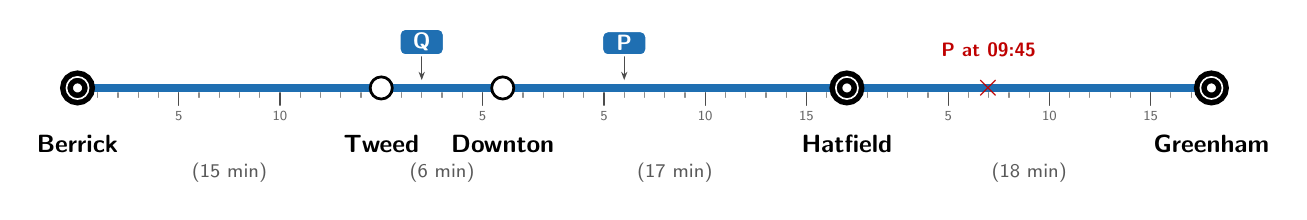
\begin{tikzpicture}[line cap=round]
\draw[a34, line width=3.2pt] (0,0) -- (14.40,0);
\draw[black!45] (0.257,-0.12) -- (0.257,-0.06);
\draw[black!45] (0.514,-0.12) -- (0.514,-0.06);
\draw[black!45] (0.771,-0.12) -- (0.771,-0.06);
\draw[black!45] (1.029,-0.12) -- (1.029,-0.06);
\draw[black!70] (1.286,-0.22) -- (1.286,-0.06);
\node[font=\tiny, text=black!60] at (1.286,-0.36) {5};
\draw[black!45] (1.543,-0.12) -- (1.543,-0.06);
\draw[black!45] (1.800,-0.12) -- (1.800,-0.06);
\draw[black!45] (2.057,-0.12) -- (2.057,-0.06);
\draw[black!45] (2.314,-0.12) -- (2.314,-0.06);
\draw[black!70] (2.571,-0.22) -- (2.571,-0.06);
\node[font=\tiny, text=black!60] at (2.571,-0.36) {10};
\draw[black!45] (2.829,-0.12) -- (2.829,-0.06);
\draw[black!45] (3.086,-0.12) -- (3.086,-0.06);
\draw[black!45] (3.343,-0.12) -- (3.343,-0.06);
\draw[black!45] (3.600,-0.12) -- (3.600,-0.06);
\draw[black!45] (4.114,-0.12) -- (4.114,-0.06);
\draw[black!45] (4.371,-0.12) -- (4.371,-0.06);
\draw[black!45] (4.629,-0.12) -- (4.629,-0.06);
\draw[black!45] (4.886,-0.12) -- (4.886,-0.06);
\draw[black!70] (5.143,-0.22) -- (5.143,-0.06);
\node[font=\tiny, text=black!60] at (5.143,-0.36) {5};
\draw[black!45] (5.657,-0.12) -- (5.657,-0.06);
\draw[black!45] (5.914,-0.12) -- (5.914,-0.06);
\draw[black!45] (6.171,-0.12) -- (6.171,-0.06);
\draw[black!45] (6.429,-0.12) -- (6.429,-0.06);
\draw[black!70] (6.686,-0.22) -- (6.686,-0.06);
\node[font=\tiny, text=black!60] at (6.686,-0.36) {5};
\draw[black!45] (6.943,-0.12) -- (6.943,-0.06);
\draw[black!45] (7.200,-0.12) -- (7.200,-0.06);
\draw[black!45] (7.457,-0.12) -- (7.457,-0.06);
\draw[black!45] (7.714,-0.12) -- (7.714,-0.06);
\draw[black!70] (7.971,-0.22) -- (7.971,-0.06);
\node[font=\tiny, text=black!60] at (7.971,-0.36) {10};
\draw[black!45] (8.229,-0.12) -- (8.229,-0.06);
\draw[black!45] (8.486,-0.12) -- (8.486,-0.06);
\draw[black!45] (8.743,-0.12) -- (8.743,-0.06);
\draw[black!45] (9.000,-0.12) -- (9.000,-0.06);
\draw[black!70] (9.257,-0.22) -- (9.257,-0.06);
\node[font=\tiny, text=black!60] at (9.257,-0.36) {15};
\draw[black!45] (9.514,-0.12) -- (9.514,-0.06);
\draw[black!45] (10.029,-0.12) -- (10.029,-0.06);
\draw[black!45] (10.286,-0.12) -- (10.286,-0.06);
\draw[black!45] (10.543,-0.12) -- (10.543,-0.06);
\draw[black!45] (10.800,-0.12) -- (10.800,-0.06);
\draw[black!70] (11.057,-0.22) -- (11.057,-0.06);
\node[font=\tiny, text=black!60] at (11.057,-0.36) {5};
\draw[black!45] (11.314,-0.12) -- (11.314,-0.06);
\draw[black!45] (11.571,-0.12) -- (11.571,-0.06);
\draw[black!45] (11.829,-0.12) -- (11.829,-0.06);
\draw[black!45] (12.086,-0.12) -- (12.086,-0.06);
\draw[black!70] (12.343,-0.22) -- (12.343,-0.06);
\node[font=\tiny, text=black!60] at (12.343,-0.36) {10};
\draw[black!45] (12.600,-0.12) -- (12.600,-0.06);
\draw[black!45] (12.857,-0.12) -- (12.857,-0.06);
\draw[black!45] (13.114,-0.12) -- (13.114,-0.06);
\draw[black!45] (13.371,-0.12) -- (13.371,-0.06);
\draw[black!70] (13.629,-0.22) -- (13.629,-0.06);
\node[font=\tiny, text=black!60] at (13.629,-0.36) {15};
\draw[black!45] (13.886,-0.12) -- (13.886,-0.06);
\draw[black!45] (14.143,-0.12) -- (14.143,-0.06);
\node[inter, minimum size=8pt] at (0.000,0) {};
\node[font=\small\bfseries, anchor=north] at (0.000,-0.48) {Berrick};
\node[busstop, minimum size=8pt] at (3.857,0) {};
\node[font=\small\bfseries, anchor=north] at (3.857,-0.48) {Tweed};
\node[busstop, minimum size=8pt] at (5.400,0) {};
\node[font=\small\bfseries, anchor=north] at (5.400,-0.48) {Downton};
\node[inter, minimum size=8pt] at (9.771,0) {};
\node[font=\small\bfseries, anchor=north] at (9.771,-0.48) {Hatfield};
\node[inter, minimum size=8pt] at (14.400,0) {};
\node[font=\small\bfseries, anchor=north] at (14.400,-0.48) {Greenham};
\node[font=\scriptsize, text=black!65] at (1.929,-1.08) {(15 min)};
\node[font=\scriptsize, text=black!65] at (4.629,-1.08) {(6 min)};
\node[font=\scriptsize, text=black!65] at (7.586,-1.08) {(17 min)};
\node[font=\scriptsize, text=black!65] at (12.086,-1.08) {(18 min)};
\draw[black!70, -{Stealth[length=3pt]}] (6.943,0.42) -- (6.943,0.1);
\node[busA, font=\footnotesize\bfseries, minimum width=16pt, above] at (6.943,0.4) {P};
\draw[black!70, -{Stealth[length=3pt]}] (4.371,0.42) -- (4.371,0.1);
\node[busA, font=\footnotesize\bfseries, minimum width=16pt, above] at (4.371,0.4) {Q};
\node[text=red!75!black, font=\large\bfseries] at (11.571,0) {$\times$};
\node[text=red!75!black, font=\scriptsize\bfseries, above=10pt, fill=white, inner sep=1pt] at (11.571,0) {P at 09:45};
\end{tikzpicture}\end{minipage}\par{\small \begin{enumerate}[label=\textbf{\alph*)}, leftmargin=*, itemsep=3pt, topsep=3pt]
\item Which bus is \textbf{P}, and which is \textbf{Q}? (Give the time each one left Berrick.) \hfill P: \aline\ \ Q: \aline\ \ \ans{P = 09:00, Q = 09:10}
\item How many minutes until bus P reaches \textbf{Hatfield}? \aline\quad \textbf{Greenham}? \aline\ \ \ans{Hatfield 11 min (09:38); Greenham 29 min (09:56)}
\item How many minutes until bus Q reaches \textbf{Downton}? \aline\quad \textbf{Greenham}? \aline\ \ \ans{Downton 4 min (09:31); Greenham 39 min (10:06)}
\item Mark with a cross ($\times$) where bus P will be at \textbf{09:45}.\ \ \ans{7 minutes past Hatfield (see cross)}
\item Tom arrives at the Tweed stop at 09:27, just as bus Q pulls away. How long must he wait for the next A34? \aline\ \ \ans{next A34 at Tweed is 10:05, so 38 minutes}
\end{enumerate}}

\banner{c18}{Zoom 2 \quad The C-18 road at 10:05}\par\smallskip\noindent\begin{minipage}[c]{0.13\linewidth}\centering 
\begin{tikzpicture}[baseline=-3pt]\draw[thick, fill=white] (0,0) circle (0.6);\draw[thick] (0.000,0.460) -- (0.000,0.600);\draw[] (0.265,0.459) -- (0.300,0.520);\draw[] (0.459,0.265) -- (0.520,0.300);\draw[thick] (0.460,0.000) -- (0.600,0.000);\draw[] (0.459,-0.265) -- (0.520,-0.300);\draw[] (0.265,-0.459) -- (0.300,-0.520);\draw[thick] (0.000,-0.460) -- (0.000,-0.600);\draw[] (-0.265,-0.459) -- (-0.300,-0.520);\draw[] (-0.459,-0.265) -- (-0.520,-0.300);\draw[thick] (-0.460,-0.000) -- (-0.600,-0.000);\draw[] (-0.459,0.265) -- (-0.520,0.300);\draw[] (-0.265,0.459) -- (-0.300,0.520);\draw[line width=1.4pt] (0,0) -- (-0.278,0.177);\draw[line width=0.8pt] (0,0) -- (0.255,0.442);\fill (0,0) circle (1.2pt);\end{tikzpicture}\\{\bfseries 10:05}\end{minipage}\hfill\begin{minipage}[c]{0.86\linewidth}\centering 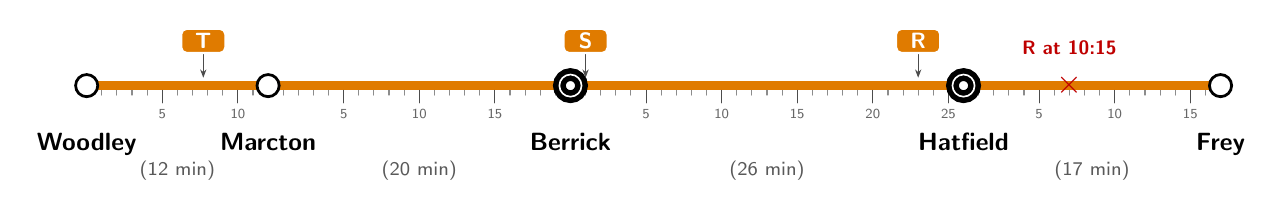
\begin{tikzpicture}[line cap=round]
\draw[c18, line width=3.2pt] (0,0) -- (14.40,0);
\draw[black!45] (0.192,-0.12) -- (0.192,-0.06);
\draw[black!45] (0.384,-0.12) -- (0.384,-0.06);
\draw[black!45] (0.576,-0.12) -- (0.576,-0.06);
\draw[black!45] (0.768,-0.12) -- (0.768,-0.06);
\draw[black!70] (0.960,-0.22) -- (0.960,-0.06);
\node[font=\tiny, text=black!60] at (0.960,-0.36) {5};
\draw[black!45] (1.152,-0.12) -- (1.152,-0.06);
\draw[black!45] (1.344,-0.12) -- (1.344,-0.06);
\draw[black!45] (1.536,-0.12) -- (1.536,-0.06);
\draw[black!45] (1.728,-0.12) -- (1.728,-0.06);
\draw[black!70] (1.920,-0.22) -- (1.920,-0.06);
\node[font=\tiny, text=black!60] at (1.920,-0.36) {10};
\draw[black!45] (2.112,-0.12) -- (2.112,-0.06);
\draw[black!45] (2.496,-0.12) -- (2.496,-0.06);
\draw[black!45] (2.688,-0.12) -- (2.688,-0.06);
\draw[black!45] (2.880,-0.12) -- (2.880,-0.06);
\draw[black!45] (3.072,-0.12) -- (3.072,-0.06);
\draw[black!70] (3.264,-0.22) -- (3.264,-0.06);
\node[font=\tiny, text=black!60] at (3.264,-0.36) {5};
\draw[black!45] (3.456,-0.12) -- (3.456,-0.06);
\draw[black!45] (3.648,-0.12) -- (3.648,-0.06);
\draw[black!45] (3.840,-0.12) -- (3.840,-0.06);
\draw[black!45] (4.032,-0.12) -- (4.032,-0.06);
\draw[black!70] (4.224,-0.22) -- (4.224,-0.06);
\node[font=\tiny, text=black!60] at (4.224,-0.36) {10};
\draw[black!45] (4.416,-0.12) -- (4.416,-0.06);
\draw[black!45] (4.608,-0.12) -- (4.608,-0.06);
\draw[black!45] (4.800,-0.12) -- (4.800,-0.06);
\draw[black!45] (4.992,-0.12) -- (4.992,-0.06);
\draw[black!70] (5.184,-0.22) -- (5.184,-0.06);
\node[font=\tiny, text=black!60] at (5.184,-0.36) {15};
\draw[black!45] (5.376,-0.12) -- (5.376,-0.06);
\draw[black!45] (5.568,-0.12) -- (5.568,-0.06);
\draw[black!45] (5.760,-0.12) -- (5.760,-0.06);
\draw[black!45] (5.952,-0.12) -- (5.952,-0.06);
\draw[black!45] (6.336,-0.12) -- (6.336,-0.06);
\draw[black!45] (6.528,-0.12) -- (6.528,-0.06);
\draw[black!45] (6.720,-0.12) -- (6.720,-0.06);
\draw[black!45] (6.912,-0.12) -- (6.912,-0.06);
\draw[black!70] (7.104,-0.22) -- (7.104,-0.06);
\node[font=\tiny, text=black!60] at (7.104,-0.36) {5};
\draw[black!45] (7.296,-0.12) -- (7.296,-0.06);
\draw[black!45] (7.488,-0.12) -- (7.488,-0.06);
\draw[black!45] (7.680,-0.12) -- (7.680,-0.06);
\draw[black!45] (7.872,-0.12) -- (7.872,-0.06);
\draw[black!70] (8.064,-0.22) -- (8.064,-0.06);
\node[font=\tiny, text=black!60] at (8.064,-0.36) {10};
\draw[black!45] (8.256,-0.12) -- (8.256,-0.06);
\draw[black!45] (8.448,-0.12) -- (8.448,-0.06);
\draw[black!45] (8.640,-0.12) -- (8.640,-0.06);
\draw[black!45] (8.832,-0.12) -- (8.832,-0.06);
\draw[black!70] (9.024,-0.22) -- (9.024,-0.06);
\node[font=\tiny, text=black!60] at (9.024,-0.36) {15};
\draw[black!45] (9.216,-0.12) -- (9.216,-0.06);
\draw[black!45] (9.408,-0.12) -- (9.408,-0.06);
\draw[black!45] (9.600,-0.12) -- (9.600,-0.06);
\draw[black!45] (9.792,-0.12) -- (9.792,-0.06);
\draw[black!70] (9.984,-0.22) -- (9.984,-0.06);
\node[font=\tiny, text=black!60] at (9.984,-0.36) {20};
\draw[black!45] (10.176,-0.12) -- (10.176,-0.06);
\draw[black!45] (10.368,-0.12) -- (10.368,-0.06);
\draw[black!45] (10.560,-0.12) -- (10.560,-0.06);
\draw[black!45] (10.752,-0.12) -- (10.752,-0.06);
\draw[black!70] (10.944,-0.22) -- (10.944,-0.06);
\node[font=\tiny, text=black!60] at (10.944,-0.36) {25};
\draw[black!45] (11.328,-0.12) -- (11.328,-0.06);
\draw[black!45] (11.520,-0.12) -- (11.520,-0.06);
\draw[black!45] (11.712,-0.12) -- (11.712,-0.06);
\draw[black!45] (11.904,-0.12) -- (11.904,-0.06);
\draw[black!70] (12.096,-0.22) -- (12.096,-0.06);
\node[font=\tiny, text=black!60] at (12.096,-0.36) {5};
\draw[black!45] (12.288,-0.12) -- (12.288,-0.06);
\draw[black!45] (12.480,-0.12) -- (12.480,-0.06);
\draw[black!45] (12.672,-0.12) -- (12.672,-0.06);
\draw[black!45] (12.864,-0.12) -- (12.864,-0.06);
\draw[black!70] (13.056,-0.22) -- (13.056,-0.06);
\node[font=\tiny, text=black!60] at (13.056,-0.36) {10};
\draw[black!45] (13.248,-0.12) -- (13.248,-0.06);
\draw[black!45] (13.440,-0.12) -- (13.440,-0.06);
\draw[black!45] (13.632,-0.12) -- (13.632,-0.06);
\draw[black!45] (13.824,-0.12) -- (13.824,-0.06);
\draw[black!70] (14.016,-0.22) -- (14.016,-0.06);
\node[font=\tiny, text=black!60] at (14.016,-0.36) {15};
\draw[black!45] (14.208,-0.12) -- (14.208,-0.06);
\node[busstop, minimum size=8pt] at (0.000,0) {};
\node[font=\small\bfseries, anchor=north] at (0.000,-0.48) {Woodley};
\node[busstop, minimum size=8pt] at (2.304,0) {};
\node[font=\small\bfseries, anchor=north] at (2.304,-0.48) {Marcton};
\node[inter, minimum size=8pt] at (6.144,0) {};
\node[font=\small\bfseries, anchor=north] at (6.144,-0.48) {Berrick};
\node[inter, minimum size=8pt] at (11.136,0) {};
\node[font=\small\bfseries, anchor=north] at (11.136,-0.48) {Hatfield};
\node[busstop, minimum size=8pt] at (14.400,0) {};
\node[font=\small\bfseries, anchor=north] at (14.400,-0.48) {Frey};
\node[font=\scriptsize, text=black!65] at (1.152,-1.08) {(12 min)};
\node[font=\scriptsize, text=black!65] at (4.224,-1.08) {(20 min)};
\node[font=\scriptsize, text=black!65] at (8.640,-1.08) {(26 min)};
\node[font=\scriptsize, text=black!65] at (12.768,-1.08) {(17 min)};
\draw[black!70, -{Stealth[length=3pt]}] (10.560,0.42) -- (10.560,0.1);
\node[busC, font=\footnotesize\bfseries, minimum width=16pt, above] at (10.560,0.4) {R};
\draw[black!70, -{Stealth[length=3pt]}] (6.336,0.42) -- (6.336,0.1);
\node[busC, font=\footnotesize\bfseries, minimum width=16pt, above] at (6.336,0.4) {S};
\draw[black!70, -{Stealth[length=3pt]}] (1.481,0.42) -- (1.481,0.1);
\node[busC, font=\footnotesize\bfseries, minimum width=16pt, above] at (1.481,0.4) {T};
\node[text=red!75!black, font=\large\bfseries] at (12.480,0) {$\times$};
\node[text=red!75!black, font=\scriptsize\bfseries, above=10pt, fill=white, inner sep=1pt] at (12.480,0) {R at 10:15};
\end{tikzpicture}\end{minipage}\par{\small \begin{enumerate}[label=\textbf{\alph*)}, leftmargin=*, itemsep=3pt, topsep=3pt]
\item Which bus is \textbf{R}, \textbf{S} and \textbf{T}? (C-18, C-18A or C-18B?) \\[3pt] R: \sline\quad S: \sline\quad T: \sline\ \ \ans{R = C-18 (09:10), S = C-18A, T = C-18B}
\item How many minutes until each bus reaches \textbf{Frey}? \\[3pt] R: \sline\quad S: \sline\quad T: \sline\ \ \ans{R 20 min (10:25), S 42 min (10:47), T 67 min = 1 h 7 min (11:12)}
\item Bus S has only just gone past Berrick. Why couldn't Karen, who was waiting at Berrick, get on it?\ \ \ans{the C-18A does not stop at Berrick}
\item Karen is still at Berrick at 10:05 and wants to get to Frey. When is the next C-18 she can catch? How long will she wait?\\[3pt] \aline\aline\ \ \ans{the 11:09 C-18; she waits 64 min (1 h 4 min) and arrives at Frey 11:49}
\item Mark with a cross ($\times$) where bus R will be at \textbf{10:15}.\ \ \ans{7 minutes past Hatfield (see cross)}
\end{enumerate}}

\banner{black!85}{Zoom 3 \quad The railway at 10:10}\par\smallskip\noindent\begin{minipage}[c]{0.13\linewidth}\centering 
\begin{tikzpicture}[baseline=-3pt]\draw[thick, fill=white] (0,0) circle (0.6);\draw[thick] (0.000,0.460) -- (0.000,0.600);\draw[] (0.265,0.459) -- (0.300,0.520);\draw[] (0.459,0.265) -- (0.520,0.300);\draw[thick] (0.460,0.000) -- (0.600,0.000);\draw[] (0.459,-0.265) -- (0.520,-0.300);\draw[] (0.265,-0.459) -- (0.300,-0.520);\draw[thick] (0.000,-0.460) -- (0.000,-0.600);\draw[] (-0.265,-0.459) -- (-0.300,-0.520);\draw[] (-0.459,-0.265) -- (-0.520,-0.300);\draw[thick] (-0.460,-0.000) -- (-0.600,-0.000);\draw[] (-0.459,0.265) -- (-0.520,0.300);\draw[] (-0.265,0.459) -- (-0.300,0.520);\draw[line width=1.4pt] (0,0) -- (-0.270,0.189);\draw[line width=0.8pt] (0,0) -- (0.442,0.255);\fill (0,0) circle (1.2pt);\end{tikzpicture}\\{\bfseries 10:10}\end{minipage}\hfill\begin{minipage}[c]{0.86\linewidth}\centering 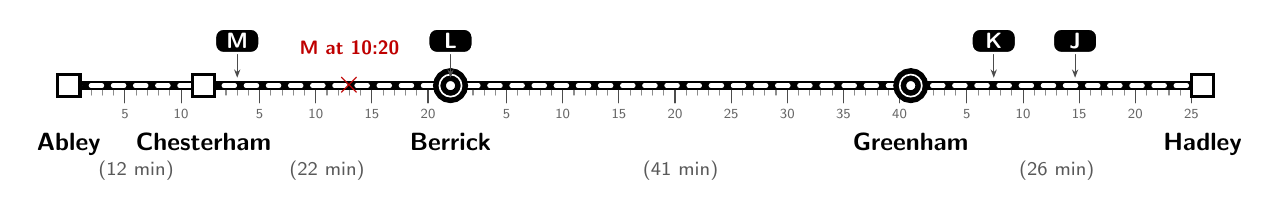
\begin{tikzpicture}[line cap=round]
\draw[black, line width=3pt] (0,0) -- (14.40,0);
\draw[white, line width=1.6pt, dash pattern=on 4pt off 4pt] (0,0) -- (14.40,0);
\draw[black!45] (0.143,-0.12) -- (0.143,-0.06);
\draw[black!45] (0.285,-0.12) -- (0.285,-0.06);
\draw[black!45] (0.428,-0.12) -- (0.428,-0.06);
\draw[black!45] (0.570,-0.12) -- (0.570,-0.06);
\draw[black!70] (0.713,-0.22) -- (0.713,-0.06);
\node[font=\tiny, text=black!60] at (0.713,-0.36) {5};
\draw[black!45] (0.855,-0.12) -- (0.855,-0.06);
\draw[black!45] (0.998,-0.12) -- (0.998,-0.06);
\draw[black!45] (1.141,-0.12) -- (1.141,-0.06);
\draw[black!45] (1.283,-0.12) -- (1.283,-0.06);
\draw[black!70] (1.426,-0.22) -- (1.426,-0.06);
\node[font=\tiny, text=black!60] at (1.426,-0.36) {10};
\draw[black!45] (1.568,-0.12) -- (1.568,-0.06);
\draw[black!45] (1.853,-0.12) -- (1.853,-0.06);
\draw[black!45] (1.996,-0.12) -- (1.996,-0.06);
\draw[black!45] (2.139,-0.12) -- (2.139,-0.06);
\draw[black!45] (2.281,-0.12) -- (2.281,-0.06);
\draw[black!70] (2.424,-0.22) -- (2.424,-0.06);
\node[font=\tiny, text=black!60] at (2.424,-0.36) {5};
\draw[black!45] (2.566,-0.12) -- (2.566,-0.06);
\draw[black!45] (2.709,-0.12) -- (2.709,-0.06);
\draw[black!45] (2.851,-0.12) -- (2.851,-0.06);
\draw[black!45] (2.994,-0.12) -- (2.994,-0.06);
\draw[black!70] (3.137,-0.22) -- (3.137,-0.06);
\node[font=\tiny, text=black!60] at (3.137,-0.36) {10};
\draw[black!45] (3.279,-0.12) -- (3.279,-0.06);
\draw[black!45] (3.422,-0.12) -- (3.422,-0.06);
\draw[black!45] (3.564,-0.12) -- (3.564,-0.06);
\draw[black!45] (3.707,-0.12) -- (3.707,-0.06);
\draw[black!70] (3.850,-0.22) -- (3.850,-0.06);
\node[font=\tiny, text=black!60] at (3.850,-0.36) {15};
\draw[black!45] (3.992,-0.12) -- (3.992,-0.06);
\draw[black!45] (4.135,-0.12) -- (4.135,-0.06);
\draw[black!45] (4.277,-0.12) -- (4.277,-0.06);
\draw[black!45] (4.420,-0.12) -- (4.420,-0.06);
\draw[black!70] (4.562,-0.22) -- (4.562,-0.06);
\node[font=\tiny, text=black!60] at (4.562,-0.36) {20};
\draw[black!45] (4.705,-0.12) -- (4.705,-0.06);
\draw[black!45] (4.990,-0.12) -- (4.990,-0.06);
\draw[black!45] (5.133,-0.12) -- (5.133,-0.06);
\draw[black!45] (5.275,-0.12) -- (5.275,-0.06);
\draw[black!45] (5.418,-0.12) -- (5.418,-0.06);
\draw[black!70] (5.560,-0.22) -- (5.560,-0.06);
\node[font=\tiny, text=black!60] at (5.560,-0.36) {5};
\draw[black!45] (5.703,-0.12) -- (5.703,-0.06);
\draw[black!45] (5.846,-0.12) -- (5.846,-0.06);
\draw[black!45] (5.988,-0.12) -- (5.988,-0.06);
\draw[black!45] (6.131,-0.12) -- (6.131,-0.06);
\draw[black!70] (6.273,-0.22) -- (6.273,-0.06);
\node[font=\tiny, text=black!60] at (6.273,-0.36) {10};
\draw[black!45] (6.416,-0.12) -- (6.416,-0.06);
\draw[black!45] (6.558,-0.12) -- (6.558,-0.06);
\draw[black!45] (6.701,-0.12) -- (6.701,-0.06);
\draw[black!45] (6.844,-0.12) -- (6.844,-0.06);
\draw[black!70] (6.986,-0.22) -- (6.986,-0.06);
\node[font=\tiny, text=black!60] at (6.986,-0.36) {15};
\draw[black!45] (7.129,-0.12) -- (7.129,-0.06);
\draw[black!45] (7.271,-0.12) -- (7.271,-0.06);
\draw[black!45] (7.414,-0.12) -- (7.414,-0.06);
\draw[black!45] (7.556,-0.12) -- (7.556,-0.06);
\draw[black!70] (7.699,-0.22) -- (7.699,-0.06);
\node[font=\tiny, text=black!60] at (7.699,-0.36) {20};
\draw[black!45] (7.842,-0.12) -- (7.842,-0.06);
\draw[black!45] (7.984,-0.12) -- (7.984,-0.06);
\draw[black!45] (8.127,-0.12) -- (8.127,-0.06);
\draw[black!45] (8.269,-0.12) -- (8.269,-0.06);
\draw[black!70] (8.412,-0.22) -- (8.412,-0.06);
\node[font=\tiny, text=black!60] at (8.412,-0.36) {25};
\draw[black!45] (8.554,-0.12) -- (8.554,-0.06);
\draw[black!45] (8.697,-0.12) -- (8.697,-0.06);
\draw[black!45] (8.840,-0.12) -- (8.840,-0.06);
\draw[black!45] (8.982,-0.12) -- (8.982,-0.06);
\draw[black!70] (9.125,-0.22) -- (9.125,-0.06);
\node[font=\tiny, text=black!60] at (9.125,-0.36) {30};
\draw[black!45] (9.267,-0.12) -- (9.267,-0.06);
\draw[black!45] (9.410,-0.12) -- (9.410,-0.06);
\draw[black!45] (9.552,-0.12) -- (9.552,-0.06);
\draw[black!45] (9.695,-0.12) -- (9.695,-0.06);
\draw[black!70] (9.838,-0.22) -- (9.838,-0.06);
\node[font=\tiny, text=black!60] at (9.838,-0.36) {35};
\draw[black!45] (9.980,-0.12) -- (9.980,-0.06);
\draw[black!45] (10.123,-0.12) -- (10.123,-0.06);
\draw[black!45] (10.265,-0.12) -- (10.265,-0.06);
\draw[black!45] (10.408,-0.12) -- (10.408,-0.06);
\draw[black!70] (10.550,-0.22) -- (10.550,-0.06);
\node[font=\tiny, text=black!60] at (10.550,-0.36) {40};
\draw[black!45] (10.836,-0.12) -- (10.836,-0.06);
\draw[black!45] (10.978,-0.12) -- (10.978,-0.06);
\draw[black!45] (11.121,-0.12) -- (11.121,-0.06);
\draw[black!45] (11.263,-0.12) -- (11.263,-0.06);
\draw[black!70] (11.406,-0.22) -- (11.406,-0.06);
\node[font=\tiny, text=black!60] at (11.406,-0.36) {5};
\draw[black!45] (11.549,-0.12) -- (11.549,-0.06);
\draw[black!45] (11.691,-0.12) -- (11.691,-0.06);
\draw[black!45] (11.834,-0.12) -- (11.834,-0.06);
\draw[black!45] (11.976,-0.12) -- (11.976,-0.06);
\draw[black!70] (12.119,-0.22) -- (12.119,-0.06);
\node[font=\tiny, text=black!60] at (12.119,-0.36) {10};
\draw[black!45] (12.261,-0.12) -- (12.261,-0.06);
\draw[black!45] (12.404,-0.12) -- (12.404,-0.06);
\draw[black!45] (12.547,-0.12) -- (12.547,-0.06);
\draw[black!45] (12.689,-0.12) -- (12.689,-0.06);
\draw[black!70] (12.832,-0.22) -- (12.832,-0.06);
\node[font=\tiny, text=black!60] at (12.832,-0.36) {15};
\draw[black!45] (12.974,-0.12) -- (12.974,-0.06);
\draw[black!45] (13.117,-0.12) -- (13.117,-0.06);
\draw[black!45] (13.259,-0.12) -- (13.259,-0.06);
\draw[black!45] (13.402,-0.12) -- (13.402,-0.06);
\draw[black!70] (13.545,-0.22) -- (13.545,-0.06);
\node[font=\tiny, text=black!60] at (13.545,-0.36) {20};
\draw[black!45] (13.687,-0.12) -- (13.687,-0.06);
\draw[black!45] (13.830,-0.12) -- (13.830,-0.06);
\draw[black!45] (13.972,-0.12) -- (13.972,-0.06);
\draw[black!45] (14.115,-0.12) -- (14.115,-0.06);
\draw[black!70] (14.257,-0.22) -- (14.257,-0.06);
\node[font=\tiny, text=black!60] at (14.257,-0.36) {25};
\node[station, minimum size=8pt] at (0.000,0) {};
\node[font=\small\bfseries, anchor=north] at (0.000,-0.48) {Abley};
\node[station, minimum size=8pt] at (1.711,0) {};
\node[font=\small\bfseries, anchor=north] at (1.711,-0.48) {Chesterham};
\node[inter, minimum size=8pt] at (4.848,0) {};
\node[font=\small\bfseries, anchor=north] at (4.848,-0.48) {Berrick};
\node[inter, minimum size=8pt] at (10.693,0) {};
\node[font=\small\bfseries, anchor=north] at (10.693,-0.48) {Greenham};
\node[station, minimum size=8pt] at (14.400,0) {};
\node[font=\small\bfseries, anchor=north] at (14.400,-0.48) {Hadley};
\node[font=\scriptsize, text=black!65] at (0.855,-1.08) {(12 min)};
\node[font=\scriptsize, text=black!65] at (3.279,-1.08) {(22 min)};
\node[font=\scriptsize, text=black!65] at (7.770,-1.08) {(41 min)};
\node[font=\scriptsize, text=black!65] at (12.547,-1.08) {(26 min)};
\draw[black!70, -{Stealth[length=3pt]}] (12.780,0.42) -- (12.780,0.1);
\node[train, font=\footnotesize\bfseries, minimum width=16pt, above] at (12.780,0.4) {J};
\draw[black!70, -{Stealth[length=3pt]}] (11.747,0.42) -- (11.747,0.1);
\node[train, font=\footnotesize\bfseries, minimum width=16pt, above] at (11.747,0.4) {K};
\draw[black!70, -{Stealth[length=3pt]}] (4.848,0.42) -- (4.848,0.1);
\node[train, font=\footnotesize\bfseries, minimum width=16pt, above] at (4.848,0.4) {L};
\draw[black!70, -{Stealth[length=3pt]}] (2.139,0.42) -- (2.139,0.1);
\node[train, font=\footnotesize\bfseries, minimum width=16pt, above] at (2.139,0.4) {M};
\node[text=red!75!black, font=\large\bfseries] at (3.564,0) {$\times$};
\node[text=red!75!black, font=\scriptsize\bfseries, above=10pt, fill=white, inner sep=1pt] at (3.564,0) {M at 10:20};
\end{tikzpicture}\end{minipage}\par{\small \begin{enumerate}[label=\textbf{\alph*)}, leftmargin=*, itemsep=3pt, topsep=3pt]
\item Which train is \textbf{J}, \textbf{K}, \textbf{L} and \textbf{M}? (Give the time each left Abley.) \\[3pt] J: \sline\quad K: \sline\quad L: \sline\quad M: \sline\ \ \ans{J 08:59, K 08:44, L 09:24, M 09:55}
\item How many minutes until each train reaches \textbf{Hadley}? \\[3pt] J: \sline\quad K: \sline\quad L: \sline\quad M: \sline\ \ \ans{J 9 min (10:19), K 20 min (10:30), L never --- it stops at Berrick, M 86 min = 1 h 26 min (11:36)}
\item Train J left Abley 15 minutes \emph{after} train K, but it is now \emph{in front}. How can you tell from the timetable that J must have overtaken K?\ \ \ans{J leaves Abley later (08:59 vs 08:44) but arrives at Hadley earlier (10:19 vs 10:30)}
\item Priya gets to Greenham station at 10:10 and wants to go to Hadley. Train K is about to go past. When is the next train she can catch, and how long will she wait? \aline\ \ \ans{the 11:10 (the 09:55 from Abley); she waits 60 min = 1 hour}
\item Mark with a cross ($\times$) where train M will be at \textbf{10:20}.\ \ \ans{13 minutes past Chesterham (see cross)}
\end{enumerate}}

\clearpage\banner{black!80}{Part C \quad Countdown boards}\par\smallskip\begin{center}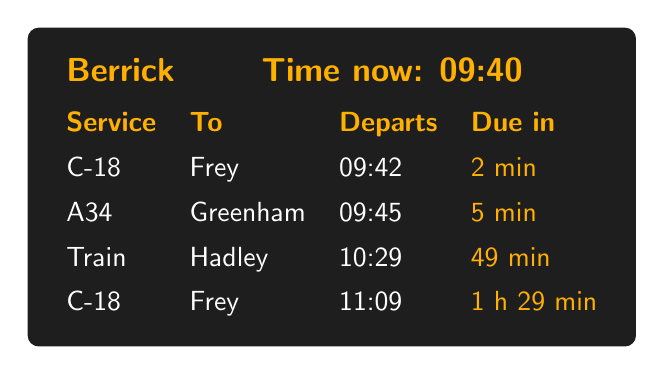
\begin{tikzpicture}\node[fill=board, rounded corners=4pt, inner sep=8pt]{\begin{tabular}{llll}\multicolumn{4}{l}{\textcolor{amber}{\bfseries\large Berrick \hfill Time now: 09:40}}\\[2pt]\textcolor{amber}{\bfseries Service} & \textcolor{amber}{\bfseries To} & \textcolor{amber}{\bfseries Departs} & \textcolor{amber}{\bfseries Due in}\\\textcolor{white}{C-18} & \textcolor{white}{Frey} & \textcolor{white}{09:42} & \textcolor{amber}{2 min}\\
\textcolor{white}{A34} & \textcolor{white}{Greenham} & \textcolor{white}{09:45} & \textcolor{amber}{5 min}\\
\textcolor{white}{Train} & \textcolor{white}{Hadley} & \textcolor{white}{10:29} & \textcolor{amber}{49 min}\\
\textcolor{white}{C-18} & \textcolor{white}{Frey} & \textcolor{white}{11:09} & \textcolor{amber}{1 h 29 min}\\\end{tabular}};\end{tikzpicture}\hspace{0.4cm}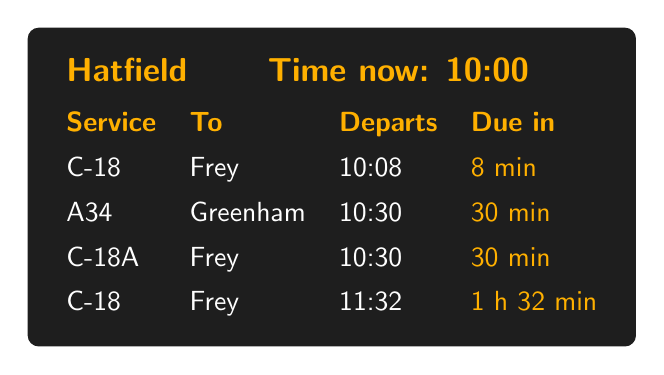
\begin{tikzpicture}\node[fill=board, rounded corners=4pt, inner sep=8pt]{\begin{tabular}{llll}\multicolumn{4}{l}{\textcolor{amber}{\bfseries\large Hatfield \hfill Time now: 10:00}}\\[2pt]\textcolor{amber}{\bfseries Service} & \textcolor{amber}{\bfseries To} & \textcolor{amber}{\bfseries Departs} & \textcolor{amber}{\bfseries Due in}\\\textcolor{white}{C-18} & \textcolor{white}{Frey} & \textcolor{white}{10:08} & \textcolor{amber}{8 min}\\
\textcolor{white}{A34} & \textcolor{white}{Greenham} & \textcolor{white}{10:30} & \textcolor{amber}{30 min}\\
\textcolor{white}{C-18A} & \textcolor{white}{Frey} & \textcolor{white}{10:30} & \textcolor{amber}{30 min}\\
\textcolor{white}{C-18} & \textcolor{white}{Frey} & \textcolor{white}{11:32} & \textcolor{amber}{1 h 32 min}\\\end{tabular}};\end{tikzpicture}\end{center}{\small \begin{enumerate}[label=\textbf{\alph*)}, leftmargin=*, itemsep=3pt, topsep=3pt]
\item Fill in the \textbf{Due in} column on both boards.\ \ \ans{see boards}
\item Lily is at Berrick at 09:40 and wants to get to \textbf{Hatfield}. Which service should she catch? What time will she arrive? \aline\ \ \ans{the C-18 at 09:42 (not the A34); arrives 10:08, 28 min after 09:40}
\item At Hatfield at 10:00, you want to get to Frey. Which bus gets you there first? How long from now until you arrive? \aline\ \ \ans{the 10:08 C-18, arriving 10:25 --- 25 min after 10:00}
\item \textbf{Make your own:} choose a stop and a time, and write a departure board for a partner to fill in.\ \ \ans{---}
\end{enumerate}}
\end{document}